\documentclass{article}
\renewcommand{\baselinestretch}{2} 

\usepackage[english]{babel}
\usepackage[letterpaper,top=2cm,bottom=2cm,left=3cm,right=3cm,marginparwidth=1.75cm]{geometry}

%Table Libraries
\usepackage{fancyhdr}
\usepackage[section]{placeins}
\usepackage{lscape}
\usepackage[table,xcdraw]{xcolor}
\usepackage{xurl}
\usepackage{graphicx}
\usepackage{float}

\usepackage{lipsum}
\usepackage{setspace}
\usepackage{etoolbox}
\preto\longtable{\par\singlespacing}


%Header and Footer Settings
\pagestyle{fancy}
\fancyhf{}
\rhead{Jasmin Martin}
\lhead{21918141}
\usepackage{lastpage}
\rfoot{\thepage\ of \pageref{LastPage}}
 \usepackage{longtable}
\usepackage{setspace}

% Useful packages
\usepackage{tikz}
\def\checkmark{\tikz\fill[scale=0.4](0,.35) -- (.25,0) -- (1,.7) -- (.25,.15) -- cycle;} 

\usepackage{amsmath}
\usepackage{graphicx}
\usepackage[colorlinks=true, allcolors=blue]{hyperref}
\graphicspath{ {./images/} }


\title{Synoptic Project Final Report}	% Title
\author{21918141}		% Author
\date{\today}			% Date

\graphicspath{{img/}}

%% Make title, author and date available via macros 
\makeatletter
\let\thetitle\@title
\let\theauthor\@author
\let\thedate\@date
\makeatother

\begin{document}
\begin{titlepage}
  \centering
  \vspace*{0.5 cm}
  
\includegraphics[scale = 0.15]{images/bucks-logo.jpeg}\\[1.0 cm]	   % University Logo
  \textsc{\LARGE Buckinghamshire New University}\\[2.0 cm]	   % University Name
  \textsc{\Large CO698WBL }\\[0.5 cm] % Course Code
  \textsc{\large BSc. (Hons) Digital and Technology Solutions Professional}\\[0.5 cm]			% Course Name
  \rule{\linewidth}{0.2 mm} \\[0.4 cm]
       { \huge \bfseries \thetitle}\\
       \rule{\linewidth}{0.2 mm} \\[1.5 cm]

       \begin{minipage}{0.4\textwidth}
	 \begin{flushleft} \large
	   \emph{Author:}\\
           Jasmin Martin (21918141)    % Author
	 \end{flushleft}
       \end{minipage}~
       \begin{minipage}{0.4\textwidth}
	 \begin{flushright} \large
	   \emph{Supervisor:} \\
           Jonathan Jackson     % Marker
	 \end{flushright}
       \end{minipage}\\[2 cm] 

       {\large \thedate}\\[2 cm]

       \vfill

\end{titlepage}

\newpage

\section*{Project Title}
\addcontentsline{toc}{section}{Project Title}
The research, design and development of a browser application, utilising natural language processing techniques, to improve documentation comprehension by transforming a hierarchical file system into an interactive graph.

\newpage

\section*{Acknowledgements}
\addcontentsline{toc}{section}{Acknowledgements}
This dissertation has been completed as part of the New Buckinghamshire University Digital Technology Solutions Professional Apprenticeship degree.

The author would like to thank their supervisor Jonathan Jackson for his continuous support throughout the development of the project. His guidance and positivity was invaluable.

Appreciation should also be extended to their employer and colleagues for providing them with the opportunity to improve their technical and professional skills.

\newpage

\section*{Abstract}
\addcontentsline{toc}{section}{Abstract}
The conventional computer file system limits the user to a hierarchical structure that may obscure the relationships between documents located within different folders. Here, the author reports the development of a browser application that transforms the file system into an interactive graph, whereby related documents are linked by common keywords. The application, called Atlas, uses natural language processing techniques to parse files and generate graphical structures that reveal the contextual relationships between documents. The author utilised the Scrumban agile methodology to iteratively develop the application by incorporating user feedback gathered from a series of presentations, surveys and interviews. By engaging in each part of the product life cycle, the author was able to design, develop and deploy Atlas into their organisation. Atlas can now be used to improve the comprehension of documentation, and in turn, increase the productivity of users.

\newpage

\tableofcontents

\newpage

\section{Introduction and Background}

The aim of the synoptic project was to create an application that could improve documentation comprehension and discovery in the author's organisation. The author designed and developed Atlas; a browser application that can transform a hierarchical file system into an interactive graph of documentation. The graph, named the Atlas Web, displays each document as a single node. Documents are connected if they contain common keywords (Figure ~\ref{fig:web-intro}). The Atlas Web reveals contextual information that could enable the user to better understand the relationships between documents and the concepts they represent. In turn, Atlas could increase the productivity of an organisation as the Atlas Web improves understanding and identifies opportunities for collaboration. 

\begin{figure}[!htb]
  \centering
      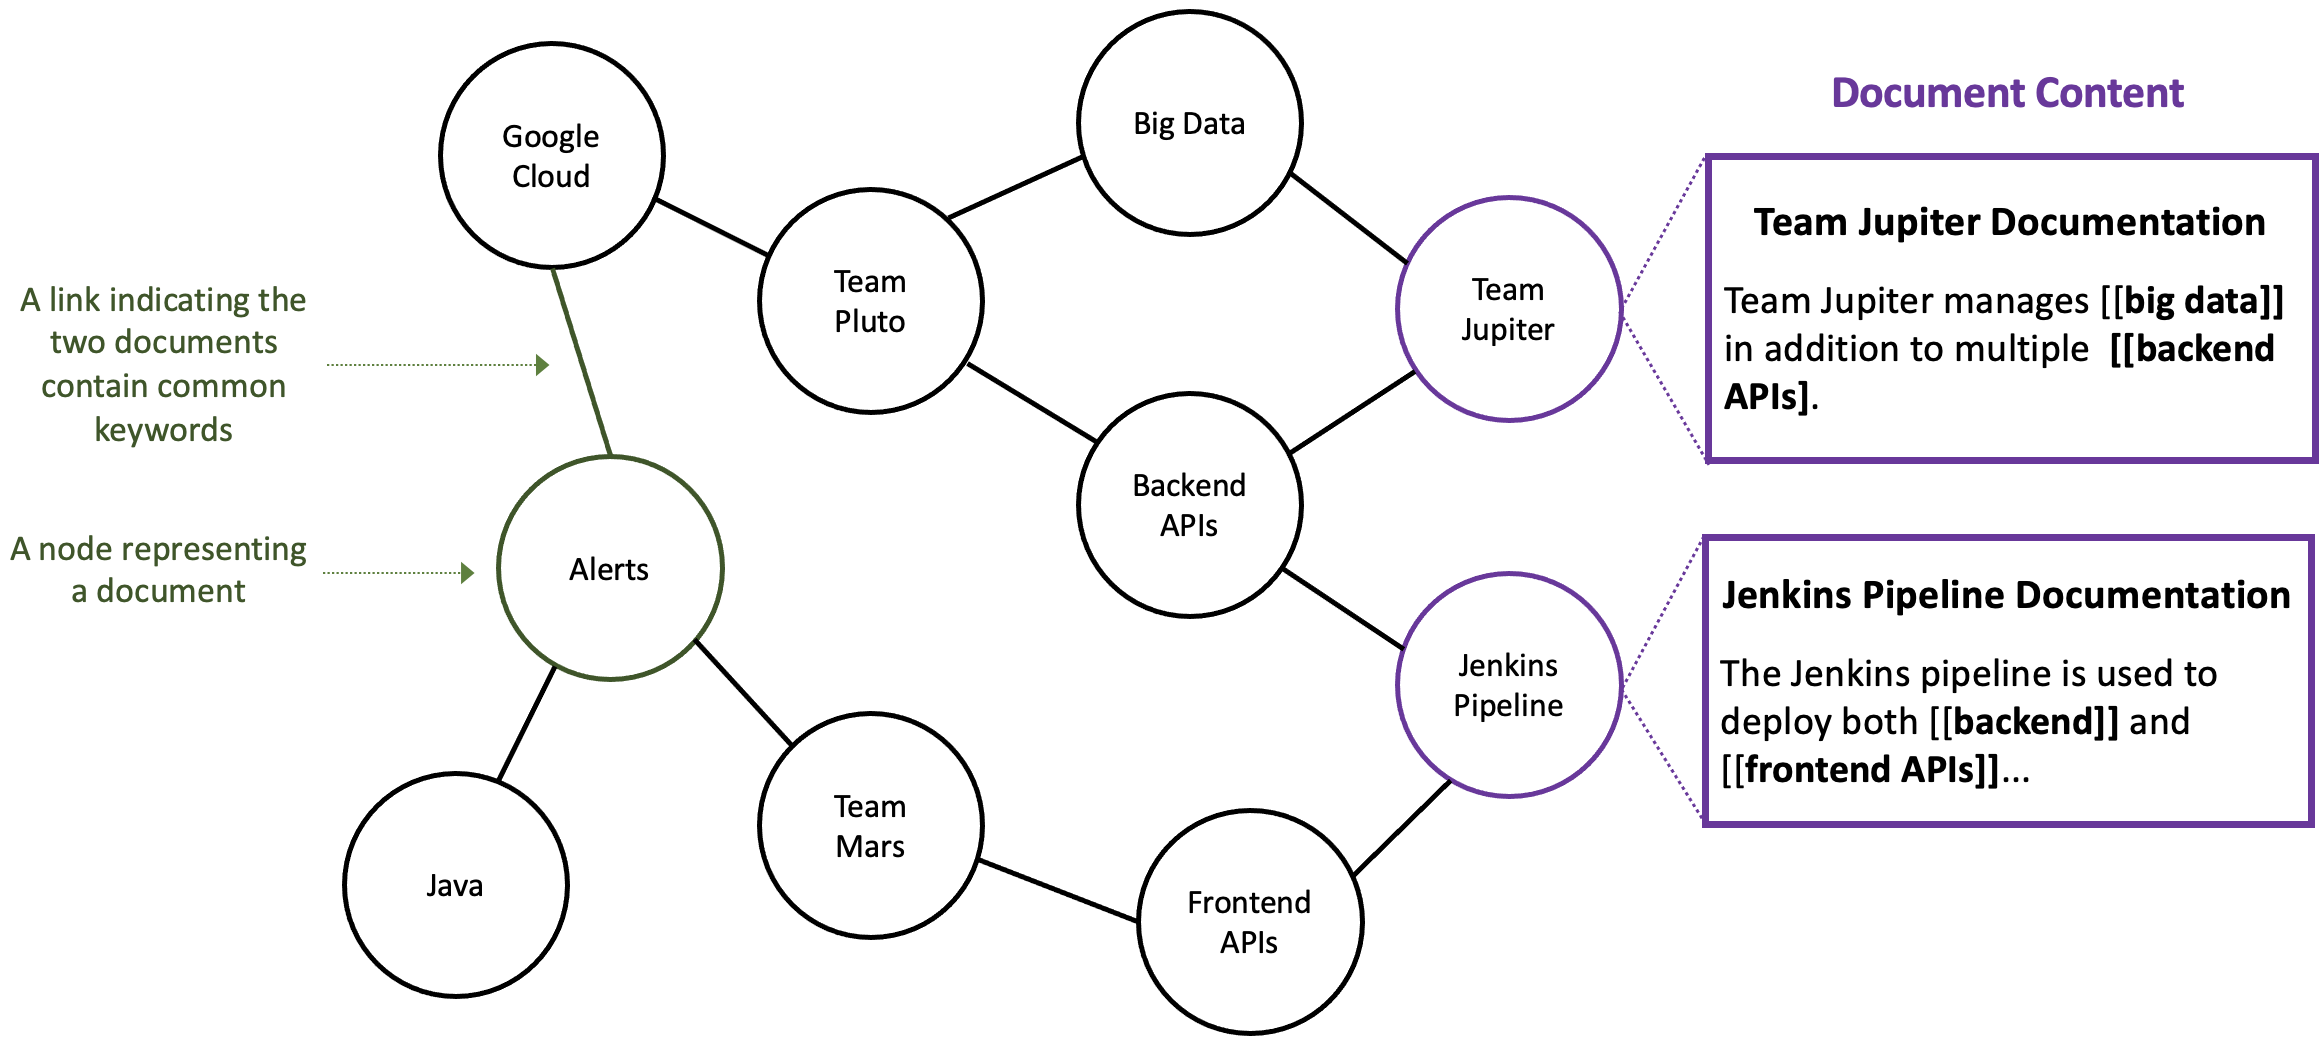
\includegraphics[width=1\textwidth]{images/atlas-web.png}
  \caption{The Atlas Web is a graph of document nodes that are linked by common keywords.}
  \label{fig:web-intro}
\end{figure}


The idea behind Atlas originated from the author's initial struggle to understand the structure of their organisation. The provided directory of documentation was disorganized and difficult to navigate. As a result, it hindered the author's ability to collaborate with different teams in their department. Disorganized file systems are a common problem for large organisations. A recent study reported 73\% of new employees believed poorly maintained document systems hindered their ability to build productive relationships (Rana et al., 2020). External knowledge management tools including Roam (White-Sullivan, 2017) an Notion (Zhao, 2016) have attempted to alleviate these issue by transforming file systems with more intuitive user interfaces. The key purpose of this synoptic project was to develop a cheaper internal solution to improve document comprehension in the author's organisation.

Atlas was designed and developed as part of the New Buckinghamshire University Digital and Technology Apprenticeship scheme. Over the course of the synoptic project, the author improved their project management and professional skills by collaborating with members of their organisation to create a product tailored to the businesses needs. The author also built upon their technical abilities by exploring natural language processing techniques to process and display large amounts of data. In this report the author describes the development process of Atlas and discusses how the project improved their skills. The accompanying software artefact can be found at \url{https://github.com/jasminmartin/atlas}. 


\newpage

\section{Strategic Rationale and Business Case}

\subsection{Business Value}

The potential user base of Atlas is inherently wide as file systems are common to nearly all computers. However, the author envisioned Atlas to be particularly beneficial to large organisations such as the author's. Larger organisations are more likely to have more complex documentation systems, which in turn, require more active management and have a greater chance of becoming disorganised. Atlas could be particularly useful to these organisations, as the Atlas Web can automatically calculate and display the contextual links between documents. These links could passively reveal untapped relationships between separate, uncoordinated areas of the organisation.

The Atlas Web is more valuable than even the most organised of hierarchical file systems, as the interface does not limit the user to the context of a folder (Figure ~\ref{fig:filesystem}). Instead, their scope is broadened to include an overview of all documents. The Atlas Web was designed to improve the productivity and efficiency of users, as they are more easily able to understand the relationships between different areas of the business. Duplicated or disorganised documentation can easily be identified within the Atlas Web, and the resulting clarifications could lead to less duplicated work and more knowledge sharing (Figure ~\ref{fig:benefits-of-web}).

\begin{figure}[!htb]
  \centering
      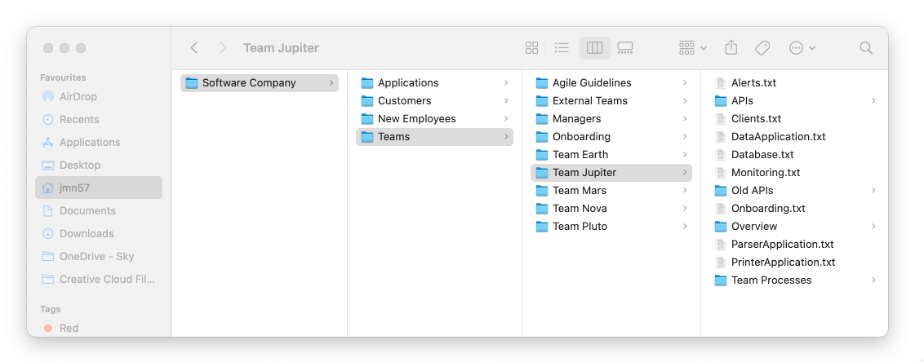
\includegraphics[width=1\textwidth]{images/filesystem-business-case.png}
  \caption{The traditional hierarchical file system limits users within the scope of folders.}
    \label{fig:filesystem}
\end{figure}

\begin{figure}[!hbt]
  \centering
      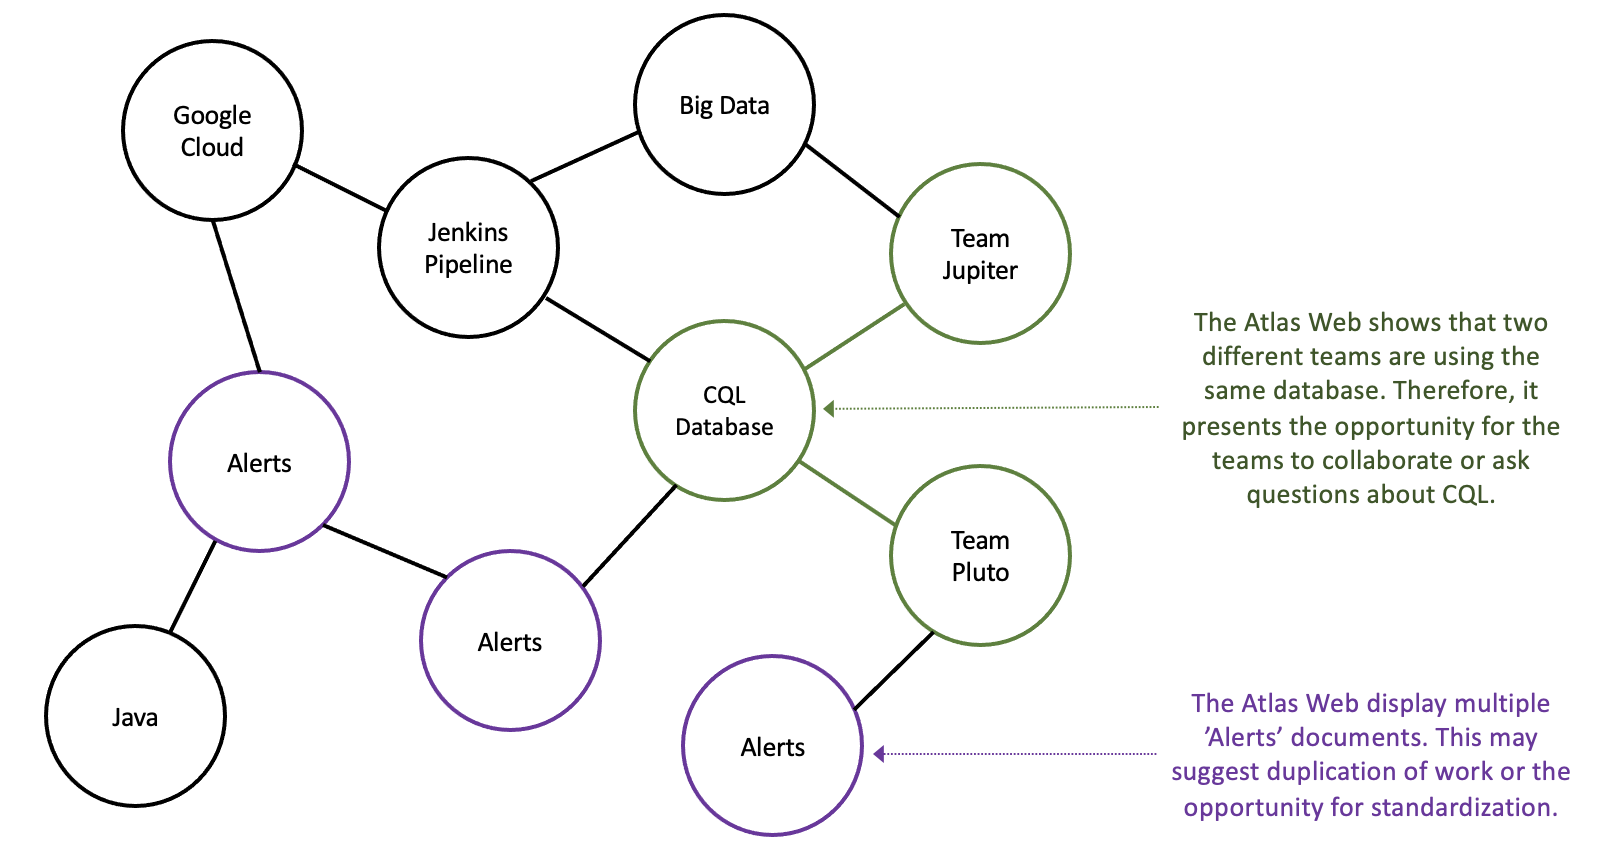
\includegraphics[width=1\textwidth]{images/benefits-of-web.png}
  \caption{The Atlas Web creates the opportunity for teams to collaborate and share knowledge.}
  \label{fig:benefits-of-web}
\end{figure}

It is important to recognise that the effectiveness of knowledge management tools is not anecdotal, rather the benefits have a scientific basis. Research has shown visual devices such as mind-maps and diagrams similar to those generated by Atlas are more effective at conveying information than text-based structures (Johnson-Laird, 1983). This preference for visual information has been proven in multiple contexts. For instance, when learning to read, children respond faster when presented with word and picture combinations, than the written words alone. Although this preference for visual word pairs fades with age, the increased comprehension of diagrammatically displayed information remains in adulthood (Coleman et al., 2018). This was confirmed by a study that revealed students taught with integrated text diagrams performed better on tests as opposed to students who were presented with text (Hegarty et al., 1991). 

Visual aids are particularly useful when representing complicated events, concepts, or relationships which would otherwise be difficult to portray with words. Although the degree of comprehension of a visual aid will increase with the individuals' cognitive aptitude and profile, generally, the presence of visual aids enables individuals to coordinate both the information from the text and the diagram to create more meaningful linkages (Schieter and Eitel, 2015). This research supports the basis that Atlas could increase the overall comprehension of documentation. Thus, a large organisation, such as the author's employer, could benefit from conveying information visually.

Atlas could become particularly effective for new employees who could utilise the Atlas Web to familiarise themselves with the organisations layout. Research suggests that employees may not become effective in their role until they have a good understanding of the organisation structure (Dohetry et al., 2010). Therefore, Atlas could become paramount in reducing the time taken and financial cost of on boarding new members of the organisation. 

\subsection{Analysis of Commercial Alternatives}

To determine whether a knowledge management tool should be purchased rather than developed in house, the author analysed competing software solutions. Several software applications offer documentation visualisation functionality, the most popular of which is Roam. Roam has been described as a “note-taking application for networked thought” (White-Sullivan, 2017) (Figure ~\ref{fig:competitors}A). Like Atlas, Roam links documents by keywords to produce an overview of all documentation. Roam gained popularity as an early visual note taking tool and was recently valued at \$200 million. Roam is used by clients such as CodeAcademy, CapgeMini and Match to support and share their large documentation structures with employees (Clark, 2020). In contrast to Roam, Obsidian is a newer freely available graph generating tool, that is available to download locally (Figure ~\ref{fig:competitors}B) (Xu, 2020).

\begin{figure}[!htb]
  \centering
      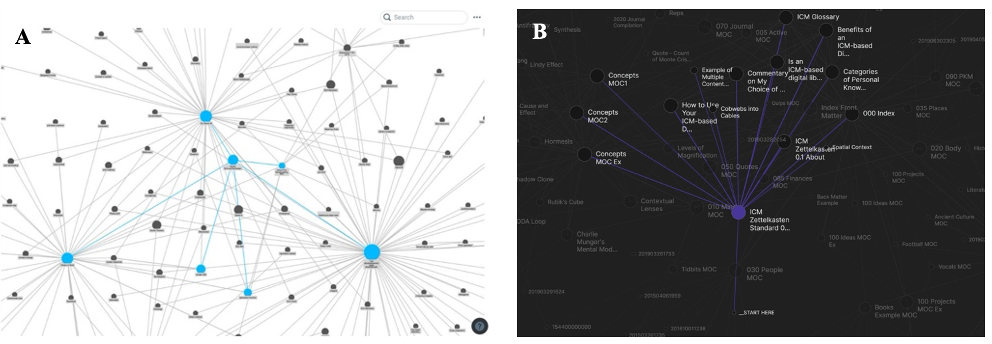
\includegraphics[width=1\textwidth]{images/roam-and-obsidian.png}
  \caption{The graphical interfaces of competing software applications offering visual document structures; Roam (A) and Obsidian (B).}
  \label{fig:competitors}
\end{figure}

Although, current documentation visualisation tools offer a similar functionality as Atlas, the development of an internal tool would be more beneficial to the author's organisation as it would be cheaper, more secure and available to easily tailor or extend to meet the organisations needs. Roam operates on a subscription based financial model. For an organisation with over 500 members, Roam can cost up to \$40 per user annually (Roam, 2021). Such contracts could lock the organisation into a costly product which may turn out not be an appropriate solution. Cheaper solutions such as Obsidian may be appropriate for smaller organisations, whose employees have a good technical knowledge. However, for an organisation with less technical employees, it is unlikely the application would be effectively used as it requires the ability to effectively use command-line tools. On further exploration, the author found the market for freely available knowledge management tools to be limited by the ability to clearly display large quantities of documentation to non-technical users. The author believed a browser based solution that could handle a large documentation base would be most appropriate for their organisation.

\subsection{Procurement}

The author's organisation procures new management tools on a monthly basis via an open forum meeting. The author raised the idea of developing a new internal knowledge management tool to the committee and was met with interest by several members. 

Typically the forum would consider the financial cost of a new product, but as Atlas was developed as part of an apprenticeship degree, they noted that there was no immediate cost to the organisation. However, after an initial development period, further development and maintenance would require financial funding. These costs are anticipated to be relatively low as the application would be functionally complete by the end of the initial development period. Furthermore, the cost of hosting the application would be relatively low, as the organisation had already negotiated a corporate contract with Google Cloud Platform. As Atlas would not have any user limits or subscription levels, this made this internal solution cheaper than the procurement of popular commercial alternatives.

\subsection{Value to Author}

The intention of Atlas was not only to create a useful product for the organisation, but also to demonstrate and improve the author's technical skills. Atlas presented the opportunity to develop and manage a greenfield project. The author purposely chose back-end technologies familiar to their organisation to improve their abilities for use in the workplace. Furthermore, as other employees were consulted for the project, the author was able to build working relationships within the organisation.

\newpage

\section{Ethical Considerations}

On the development of software, it is vital to ensure permissions are obtained, identities are obscured and confidentiality is maintained (Winter, 1995). When consumer research was conducted for Atlas, the author ensured that all participants in the research were aware of the intentions of the project. To ensure the confidentiality of those who engaged in any research or testing of Atlas, no person was named in the report. As both the project and report were independent of others’ work, no descriptions of other projects were negotiated with any other person. 

As Atlas parsed user inputted files, it was important to ensure that the content was secure. Atlas did not utilise a database, rather the application was compiled locally and files were stored in memory on the users machine. Therefore there was no concern for the safety of the data as it could not be accessed by external parties. To prevent the misuse of the local artefact, the author conducted a testing and security analysis which resulted in upgrades to all dependencies to versions with no known security flaws.

All libraries utilised by Atlas were published via free and open source licenses. A list of them can be found in the Atlas GitHub repository.

The ethical checklist required for the synoptic project can be found in \hyperref[sec:appendix-2]{Appendix 2}.

\newpage

\section{Aim and Objectives}

\subsection{Project Aim}

The aim of the synoptic project was to create a browser application that could transform a file system into an interactive graph of documents linked by common keywords. The graph, known as an Atlas Web, would clearly demonstrate the relationships between different documents and as a result would improve the documentation comprehension and collaboration within the author's organisation. The author aimed to design, develop and deploy the greenfield product within their organisation. Atlas could then be used throughout different departments and become maintained by a team of developers.

\subsection{Project Objectives}

The author outlined four objectives at the start of the synoptic project that encompassed the product design, development and deployment.

O1. Design a graphical user interface that clearly demonstrates the relationships between documents connected by common keywords.

O2. Develop a minimal viable product that can transform a local file system into an Atlas Web.

O3. Gather and incorporate user feedback on the minimal viable product to develop improved iterations of the application that contain user requested features.

O4. Deploy Atlas into a production environment so that it can be used by organisation members. 

\newpage

\begin{landscape}

\section{Risk Management}
\singlespacing

\begin{longtable}{|p{0.6cm}|p{2cm}|p{3.3cm}|p{3.3cm}|p{3cm}|p{3.5cm}|p{3.3cm}|}
\hline
\textbf{Id} &
  \textbf{Description of Risk} &
  \textbf{Likelihood} &
  \textbf{Risk Resolution Action} &
  \textbf{Impact on Project Aim} &
  \textbf{Impact on Project Objectives} &
  \textbf{Impact on Project Plan} \\ \hline
\endhead
%
\rowcolor[HTML]{FF7E79} 
R1 &
  Underestimate the author's ability to implement the front-end design &
  High – The author had little experience with front-end development. They had previously   only developed two small front-end applications as part of their university work. &
  Mitigate – This risk was mitigated as the author chose a front-end language they had basic   experience with. This reduced the upfront learning period. &
  The user interface of Atlas could remain incomplete, or may not reflect the author's   design. The Atlas Web would not aid document comprehension. &
  The user interface may not clearly depict the relationships between documents (O1). User   feedback on the user interface may not be implemented as desired (O3). &
  The author would have to allocate more time to the front-end development or simply produce a static implementation. The intended user interface design would then be shown in the report. \\ \hline
\rowcolor[HTML]{FFC000} 
R2 &
  Underestimate the ability of the chosen technology to efficiently generate the Atlas Web &
  Moderate – The author chose the technology based on both their experience level and the outlined performance metrics. &
  Avoid – The author avoided this risk as they tested the effect of each technology on the application performance. Inefficient technologies were substituted. &
  The product may not improve the comprehension of users if it cannot efficiently generate the   Atlas Web. &
  Atlas may not be able to generate the Atlas Web efficiently (O2), resulting in a poor user experience. &
  The author would allocate more time to substitutions of inefficient technologies to   avoid poor performance. \\ \hline
\rowcolor[HTML]{92D050} 
R3 &
  Inadequate user engagement &
  Low – The author requested that their team took part in the presentations of Atlas. This guaranteed feedback from 8 users. &
  Avoid – The author avoided this risk as they gained the interest of several prospective users whom agreed to test the application. &
  The product may not be suitable for users in the business and may not improve documentation comprehension. &
  The future iterations of the application would not implement user feedback (O3). Without feedback, the app may not be suitable or desirable for improving document   comprehension. &
  The author would allocate more time to finding prospective users to test the application. They may have to utilise less feedback which in turn, could decrease the product's accessibility. \\ \hline
\rowcolor[HTML]{92D050} 
R4 &
  Inadequate time management &
  Low – The author scheduled the project development alongside their other apprenticeship modules and work requirements. &
  Mitigate – This risk was mitigated as the author incorporated the demands of the other university and work into the development plan, and included buffer period to allow for over-running development. &
  Inadequate time management could reduce the number of features implemented and potentially result in an incomplete product that could not transform a file system into an Atlas Web. &
  Dependent on the severity of disruption, inadequate time management could prevent the development of a minimal viable product (O2), future versions of the product   (O3), or the deployment (O4). &
  Inadequate time   management could push out development stages of the plan further into the future, and could risk the application not being completed in the development period. \\ \hline
\rowcolor[HTML]{FFC000} 
R5 &
  Poor code quality &
  Moderate - The author was experienced in their back-end language choice. However, they were unfamiliar with the front-end language and could not receive feedback on their code quality. &
  Mitigate – The author mitigated the risk of poor code quality as they researched and implemented good coding practices for both the front-end and back-end   languages. &
  Poor code quality could make the application difficult to maintain and debug. This could reduce the value of the product if it could not be used in the future by the organisation. &
  The author could struggle to develop the minimal viable product (O2) or future iterations if they are unable to debug issues due to poor code quality (O3). &
  Poor code quality could cause bugs that may push out the development plan. Furthermore, it may reduce the maintainability of the code for future developers. \\ \hline
\rowcolor[HTML]{FFC000} 
R6 &
  Lack of ownership &
  Moderate – The author planned to demonstrate the application to the department to find a team to maintain the product. &
  Mitigate – The author mitigated a future lack of ownership in the product as they created regular presentations on the product’s development. &
  A lack of ownership of the product could lead to knowledge silo’s and the   discontinuation of the product on completion. &
  The maintenance of the application may be disregarded if the product does not have departmental ownership (O3). &
  A lack of ownership within the department could lead to the retirement of the product as it is not adequately maintained. \\ \hline
\end{longtable}
\end{landscape}

\newpage

\section{Literature Survey}

In this literature survey the author explores the theory, technology and project management techniques that were used in the design and development of Atlas. In order to meet the outlined aims and objectives, the author explored unfamiliar technical areas such as natural language processing and artificial intelligence. To ensure the appropriate project management style was selected, the author reviewed popular management styles and selected the appropriate method.

\subsection{The Algorithm Behind Atlas}

The underlying algorithm that connects related documents in the Atlas Web is based on the Zettelkasten method. The Zettelkasten method was developed by Niklas Luhmann (1927 – 1998) (Ahrens, 2017). Luhmann was a prolific sociologist who championed neither the short or long-term memory of the human brain could comprehend large quantities of data (Ludecke, 2015). To develop a more intelligible solution to storing and organising notes, he developed the Zettelkasten method. The Zettelkasten method states a single index card contains one idea, which would be singularly referenced by a sequential number (i.e. 1). If a new note was to be made with the same theme, Luhmann then added a new index card and appended the reference with a letter (i.e. 1a). Then, if another noted related to the branched index card, it would then be similarly be referenced to (i.e. 1b) (Figure ~\ref{fig:zettelkasten}). The output of the Zettelkasten method is a database of index cards that can be extended indefinitely in any direction as each index card pertained to a static reference (Forte, 2020). 

\begin{figure}[!htb]
  \centering
      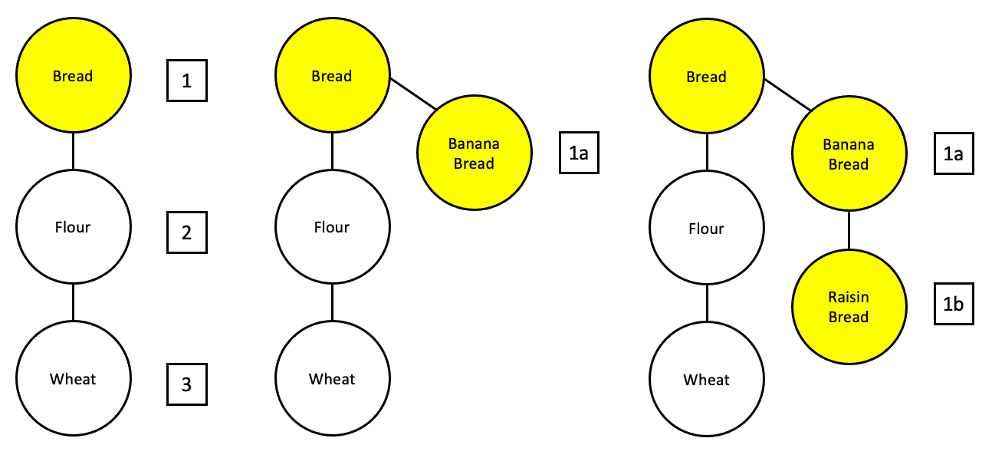
\includegraphics[width=1\textwidth]{images/litreview-zettelkasten.png}
  \caption{Niklas Luhmann’s Zettelkasten method enables users to create a database of notes, linked by topic. This is the foundation of the algorithm used by Atlas.}
  \label{fig:zettelkasten}
\end{figure}

The  Zettelkasten method produces a fluid but organised network of notes. The relationships between notes are clearly displayed, making each note more valuable as ideas are organised into reusable and reflective threads (Gibson, Gregory, and Robson, 2005). The graph of relationships provides a clear external basis of existing knowledge which compliments a more natural thought process as users can focus on elaborating ideas (Gibson, 2020). In turn, this can increase productivity as knowledge is gained more quickly and users can make more informed decisions (Glaser and Strauss, 1967). A key benefit of creating an application that uses this algorithm is that the referencing is automated. Therefore, instead of storing and searching for physical cards to reveal information, Atlas will calculate and display the relationship instantly.

A potential criticism of the Zettelkasten method is that the user may find that they are creating ideas that are contradictory or paradoxical. For instance, a user may find that two notes exist, with differing information. However, it could be argued that this is not a limitation of the Zettelkasten method, rather it is a feature. The Zettelkasten method brings these contradictions to light, adding ideas to a discussion. Contradictory data is valuable to discussions, as it represents a misalignment of knowledge and often opens new paths of inquiry (Forte, 2020). By placing incompatible theories side by side, the method encourages objectivity and shares perspectives. This independent thinking counteracts confirmation bias – our tendency to just believe information that we already know – and forces the user to confront misunderstandings (Gibson, Gregory and Robson, 2005). If Atlas was used in a large corporation, the revelation of contradictory or duplicated notes could lead to discussions or collaboration to align team and departmental knowledge.


\subsection{Project Management Techniques}

Software project management techniques are both the science and art of planning and directing software projects (Wasserman, 2010). To be effective, software project management techniques should account for the whole project life; from the initial product design, to the planning of tasks, effort estimation, work supervision, and the testing of the end product (Dyba, Dingsoyr and Moe, 2014). Such management practices have been developed with a culmination of years of trial and error. Although each technique may differ in practice, they all share the ultimate goal of building better software (Hoda, Noble and Marshall, 2008).

The agile development approach was used to develop Atlas. In agile development, developers work with end-users to implement functionality in iterative cycles. Rather than having a fixed plan,  developers respond to changing requirements in real-time (Stellman and Greene, 2008). This ethos reflects the principles outlined by the original Agile Manifesto (Fowler and Highsmith, 2000). The agile methodology opposes the traditional well-defined linear sequence of activities that traditional management techniques such as Waterfall define. Instead, the agile methodology recognises that activities may require a shorter time between planning and execution. As a result, planned features do not contain all the details of the implementation and are not planned far in advance (Hoda, Noble and Marshall, 2008). 

A particular offshoot of agile known as Scrumban was selected as the appropriate project management technique for Atlas. Scrumban is an amalgamation of two popular agile practices; Scrum and Kanban (Table 2). Both of these practices promote the fundamental agile tenant of utilising iterative and incremental techniques to quickly gain feedback on development cycles. The Scrum process defines specific individual roles, work requirements and time boxes that define clear developmental goals. Kanban, on the other hand, offers a system for visualizing a continuous flow of work. Scrumban provides the structure of Scrum and flexibility and visualization of Kanban. 

\begin{table}[!b]
\caption{An overview of Scrum, Kanban and Scrumban development methodologies. Highlighted cells reflect the chosen management techniques. Content adapted from Arbaham, 2021.}

\centering
\resizebox{\textwidth}{!}{%
\begin{tabular}{|l|l|l|l|}
\hline
 & \textbf{Scrum} & \textbf{Kanban} & \textbf{Scrumban} \\ \hline
\textbf{Timebase} & \cellcolor[HTML]{92D050}1- 4 weeks & No time base & 3 month buckets \\ \hline
\textbf{Rules} & Constrained process & Flexible process & \cellcolor[HTML]{92D050}Slightly restricted process \\ \hline
\textbf{Roles} & \begin{tabular}[c]{@{}l@{}}Product owner, scrum master,\\  scrum team, stakeholder\end{tabular} & No specific roles required & \cellcolor[HTML]{92D050}No specific roles required \\ \hline
\textbf{Board} & Defined/resets each week & Persistent – the Kanban board & \cellcolor[HTML]{92D050}Persistent – the Scrumban board \\ \hline
\textbf{Prioritization} & \cellcolor[HTML]{92D050}Backlog & Optional & Recommend on each planning \\ \hline
\textbf{Estimation} & Before sprint starts & Optional & \cellcolor[HTML]{92D050}Optional \\ \hline
\textbf{Planning routine} & Sprint planning & On demand & \cellcolor[HTML]{92D050}On demand \\ \hline
\textbf{Performance metrics} & Burn down & Cumulative flow diagram & \cellcolor[HTML]{92D050}Average cycle time \\ \hline
\end{tabular}%
}
\end{table}

The development of Atlas was well suited to Scrumban as the project exhibited a high variability in requirements, skills, and technologies (Augustine et al., 2005). Therefore, Scrumban would provide a clear progression of the project tasks. Progression awareness was particularly important for Atlas as the project was developed intermittently by a single developer. Furthermore, the short development cycles, common to agile practices, enabled the user to quickly gain user feedback. These different perspectives enabled the quick identification of problem areas and the subsequent prioritisation of features (Asra, Sobia, and Khan, 2014). 

The author deviated slightly from the pure Scrumban style, as they favoured two key Scrum aspects: a shorter iteration cycle of two weeks and the presence of a backlog. The smaller development cycles and backlog promoted more forward planning and helped the author remain organised. In addition to Scrum and Kanban, the author also took up the Extreme Programming practice of utilising spikes. Spikes are time-boxed explorations into technologies or solutions (Jeffries, 2001). Spikes were appropriate for Atlas as the author was exercising weaker skills - such as front-end development - that required further research before committing to a technical solution.

\subsection{Natural Language Processing}

In this project, the author researched natural language processing techniques. Natural language processing (NLP) is a sub-field of computer science that revolves around analysing, processing and representing human language (Damerau and Indurkhya, 2010). Researchers of natural language processing apply machine learning algorithms to speech and text to achieve human-like language processing (Chowdrhy, 2005). The application of NLP research includes predictive typing, speech recognition, and spam detection (Ventsislav, 2018).

The fundamental feature of Atlas is the ability to transform a hierarchical file system structure into the Atlas Web. To achieve this, all folders and documents in the file system must be scanned and keywords must be identified and stored. In the field of NLP, this process is known as deductive parsing (Trujillo, 2018). A deductive parsing algorithm has two distinct elements: a parser which will scan each word, and a tokenizer which will check for pre-defined tokens in the input (Chowdrhy, 2005). For Atlas, the keywords identified by the tokenizer were surrounded by square brackets (e.g. [[keyword]]).

In addition to parsing and tokenisation, Atlas would also be developed to utilise the natural language processing techniques: stemming and lemminisation. The goal of both stemming and lemmatization is to reduce inflectional forms of words in order to form a common base (Jivani, 2011). These processes would be integral to Atlas, as they would link multiple derivatives of the same word in the Atlas Web. Understanding the subtle difference between these two processes was important in order to prioritise and implement the techniques (Figure ~\ref{fig:stemlem}). Stemming is the crude process of removing the end of words, in order to chop off derivational affixes (i.e. ‘run’ and ‘running’). Lemminisation is a more complex process that conducts a morphological analysis of words, removing inflectional suffixes to return the dictionary for a word known as a lemma (i.e. ‘study’ and ‘studies’) (Ventsislav, 2018). This research led the author to prioritise, implementation of stemming first, with the goal of implementing the more complex lemminisation for the end product.

\begin{figure}[!htb]
  \centering
      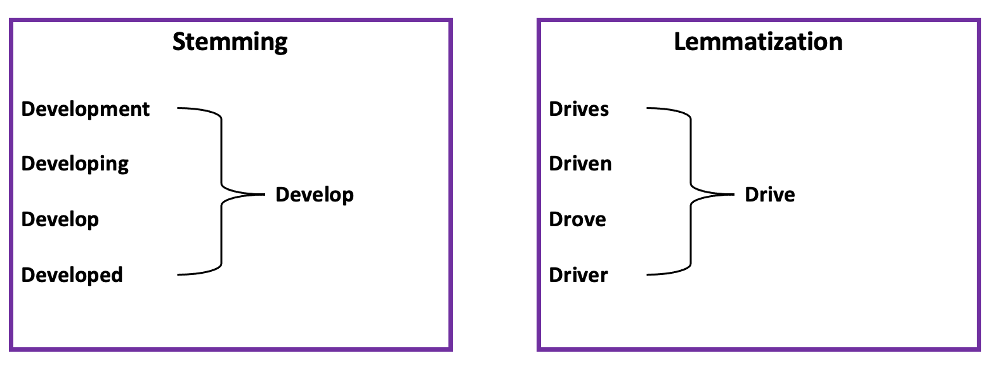
\includegraphics[width=1\textwidth]{images/litreview-nlp.png}
  \caption{The difference between two common natural language processing techniques: stemming and lemminisation.}
  \label{fig:stemlem}
\end{figure}

\subsection{Artificial Intelligence}

Atlas would incorporate elements of artificial intelligence as it would be able to recommend common keyword tags. Artificial intelligence enables machines to complete tasks that would require intelligence if completed by a human (Boden, 1997). A famous though experiment that encompasses artificial intelligence was demonstrated by Alan Turings' Imitation Game; a computer programme that displayed intelligence by deceiving a human interrogator into believing they were communicating with a human (Turing, 1950). Another example in the field of artificial intelligence expanded from rule-based systems with the advancement of neural networks. Neural networks are based on a series of algorithms, loosely modelled from the human brain, that interpret patterns from raw data.

The implementation of artificial intelligence into Atlas will improve upon the underlying Zettelkasten algorithm by automatically detecting common, non-tokenized, keywords and suggesting them to create new links between documents. This tag suggestion feature will parse all of the files and identify commonly used words using rule-based logic. Importantly, the application must identify and omit words such as 'the', 'a' and 'and' to prevent the recommendation of useless tags. This functionality will demonstrate a level of intelligence, as the application automates a task that would take a human significantly more effort  to complete.

\subsection{Language Choice}

Upon embarking on a greenfield software project, it is important to ensure the appropriate technology is chosen to meet the functional and non-functional requirements. The development of Atlas was divided into two parts, the front-end and the back-end. The back-end performed the transformation of documentation into the an object that represented the Atlas Web. Scala was selected as the back-end language as it was familiar to the author and highly performant. Scala is both a functional and object-orientated high level language which runs on the JVM. It has access to the ecosystem of Java libraries, and it is on average 20\% more performant than Java (Roper, 2012). Scala libraries such as Akka are designed to utilise resources efficiently by leveraging actor systems asynchronous thread management  which in turn makes applications highly scalable and responsive (Roestenburg et al., 2016). As Scala is statically typed, it is able to check for common classes of errors at compile time, unlike other common back-end languages such as Python (Kerringham and Ritchie, 1978). Although other back-end languages could have been used to build Atlas, the author was keen to improve and demonstrate their skill with Scala as they are utilised in their day job.

The front-end of Atlas rendered the Atlas Web. The author had little experience with front-end development, so selected React Typescript as their front-end framework. React is a library for building user interface components. It is the most popular front-end library and has a strong online community which offers a large amount of beginner support online (Pitaliya, 2021). The author selected React as they had a small amount of prior experience with it and felt confident they could create the Atlas with the online resources available. As the Atlas web could be divided into a few repeated components, the author was confident React’s reusable component system could create the interface with minimal additional complexity to the code. The author decided to choose React Typescript, the superset of JavaScript, as it adds static types to the code which in turn reduce the chance of runtime errors (Finley, 2012). Other front-end options such as Swift or Angular could have been performant enough for Atlas, but they were not selected as they would require more time for the author to develop due to their lack of experience.

\newpage

\section{Methodology}

\subsection{Timeline}

Although the development of Atlas utilised an agile project management approach, the author created an initial timeline of the development to ensure that the product could be completed before the deadline (Figure ~\ref{fig:timeline}). The timeline was flexible to allow for any unforeseen problems, and included key milestones for gathering feedback. The author purposefully ensured that the minimal viable product was created early in the development process, so they could quickly gain user feedback. Feedback was collected in different formats including a survey, focus groups, and an interview. The author planned to create three incremental versions of the application, each one included improved and additional features. The timeline also scheduled regular discussions with the project supervisor and the author's manager to ensure the project aligned with the remit and progressed the developer's skill-set.

\begin{figure}[!h]
  \centering
      \includegraphics[width=1\textwidth]{images/methodology-timeline.png}
  \caption{The original timeline outlined design and development milestones of the project.}
  \label{fig:timeline}
\end{figure}

\subsection{Scrumban Approach}

The discussion in the literature survey concluded that the Scrumban approach would be the appropriate project management style for the development of Atlas. Scrumban is a subset of agile development that uses iterative development cycles which perpetuate adaptive responses to user feedback (Stellman and Greene, 2008). The author tracked the work completed in each iteration on a GitHub KanBan board (Figure ~\ref{fig:ticket}). The Kanban board enabled the author to create tickets which detailed acceptance criteria (Figure ~\ref{fig:board}). The author decided not to explicitly estimate the tickets as there was little value to be gained as they were the sole developer and had nobody to coordinate with. Instead, they focused on creating tickets with less than 4 hours of work to ensure that they did not remain on a single ticket for a long period of time. Furthermore, the author did not abide to strict sprint timelines, instead, they aimed to spend no more than 6 weeks on each iteration of  Atlas, and added to the backlog of tickets when necessary. Although there are more detailed and trackable Kanban board solutions, GitHub was selected as it provided the required features and was conveniently hosted within the code repository. 

\begin{figure}[!htb]
  \centering
      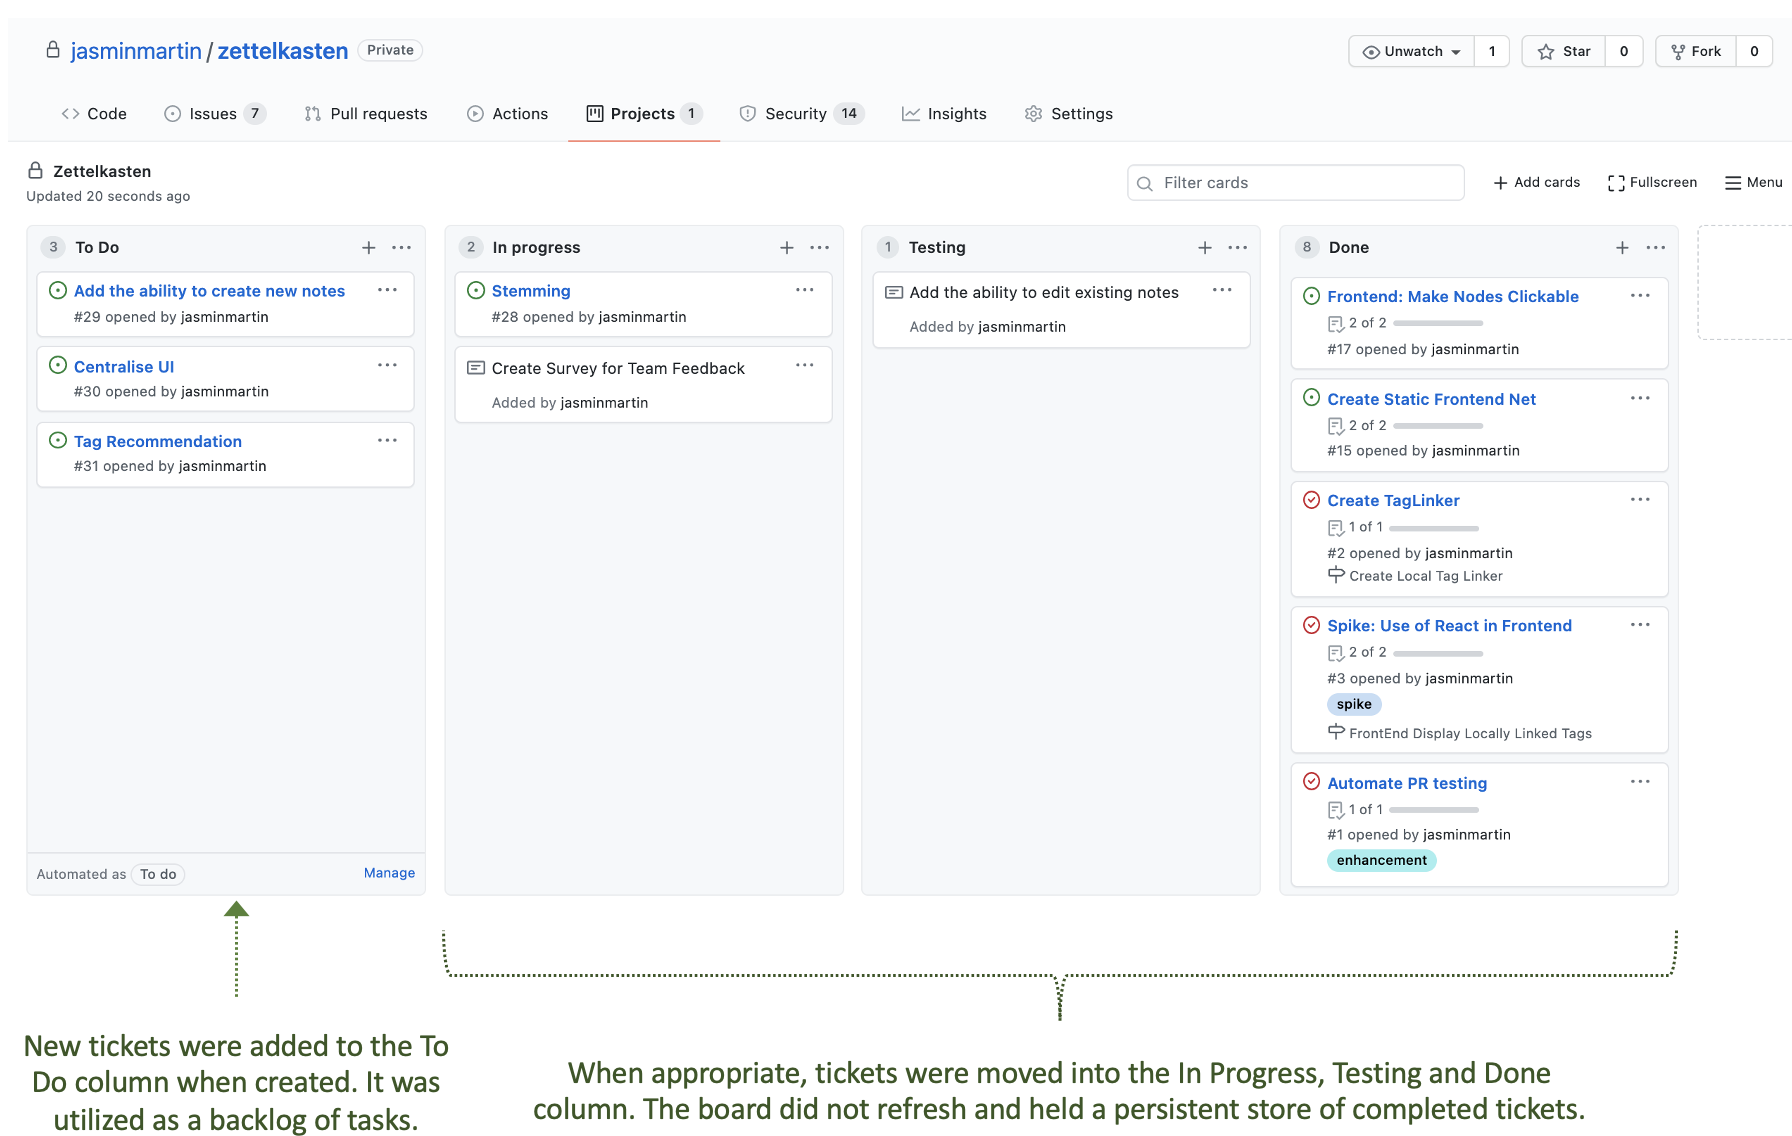
\includegraphics[width=1\textwidth]{images/methodology-ticket.png}
  \caption{The GitHub Kanban board used to track upcoming and completed tickets.}
  \label{fig:ticket}
\end{figure}

\begin{figure}[!b]
  \centering
      \includegraphics[width=1\textwidth]{images/methodology-ticket-2.png}
  \caption{Each ticket outlined acceptance criteria which defined when a card could be completed.}
    \label{fig:board}
\end{figure}

\newpage
\subsection{Incorporating User Feedback}

The incorporation of user feedback is a key tenant of agile development (Stellman and Greene, 2008). Both oral and written feedback were captured during the development of Atlas. Once the minimal viable product was complete, the author showcased the application and collected feedback in a survey. The survey captured mainly quantitative data, as closed multiple choice questions prompted the respondent to rate the demoed user experience. Qualitative feedback was captured too, in a series of open questions which enabled the user to give more detailed opinions on the current and upcoming features. Both types of data were analysed to provide the author with an idea of the user’s needs and preferences. The results of the survey influenced the features incorporated into the second version of the application, and resulted in the refinement of the features included in the minimal viable product.

Further feedback was captured in a focus group and an interview. As these two types of data collection required real-time feedback, they prompted more honest and detailed responses than the initial survey (Dawson, 2015). These demonstrations enabled the users to interact with Atlas, which in turn identified difficulties with the user experience. Live data collection was particularly important for the development of Atlas, as only a single developer created and designed the product. Incorporating other perspectives and viewpoints on the functionality made the product more valuable to a larger audience. The author decided to schedule a focus group for the end of version 2 development and later an interview for version 3, as the interview would elicit more in depth and opinionated reviews (Cottrell, 2014). The notes collected on opinions, questions, and ideas were analysed to determine any recurring themes which were addressed in the later versions of Atlas.

\newpage
\section{Requirements and Design}

Here the author describes the requirements solicitation process which shaped the design of Atlas. The initial product idea stemmed from the author's personal experience of struggling to comprehend a large, complex, hierarchical file system of documentation. As a result, the initial requirements were largely formed from the author's desire to demonstrate the benefits of generating the Atlas Web structure. Later iterations of Atlas incorporated user feedback - following the agile ethos of continuously tailoring the product to the user needs (Stellman and Greene, 2008). In this section, the author details how the user feedback influenced each iteration of the product.

\subsection{Iteration 1: MVP Concept}

The initial functionality of Atlas was demonstrated in the minimal viable product (MVP). A MVP is a product with enough features to attract customers to validate the base functionality. The key purpose of a MVP is to enable the maximum amount of user feedback with the least amount of effort (Ries, 2009). The MVP was targeted towards adults with low technical experience. This demographic was selected as research into competitor products revealed the popular knowledge management tools expected a moderate degree of technical literacy. As a result, the author purposefully limited the number of steps in the user journey required to generate the Atlas Web (Figure ~\ref{fig:competitor}). 

\begin{figure}[!t]
  \centering
      \includegraphics[width=1\textwidth]{images/workflow.png}
  \caption{The author compared the user journeys of graph generation for Atlas and it's competitor product Roam. The author intended to make Atlas's user journey simpler and more accessible.}
  \vspace*{4in}
  \label{fig:competitor}
\end{figure}

The author recognised the key features of Atlas with the aid of product wire frames (Figure ~\ref{fig:wireframe}). The original design of the Atlas web connected documents with common keywords; and displayed both the keyword and the name of the document in the Atlas web. The Atlas Web was designed to clearly depict keywords in orange boxes, and documents in multi-coloured circles. From this visual depiction, the author recognised the two key functional requirements to be the ability to form relationships between documents and keywords (F1) and the ability to display the Atlas web on the user interface (F2) (Table 3).

\clearpage

\begin{figure}[!t]
  \centering
      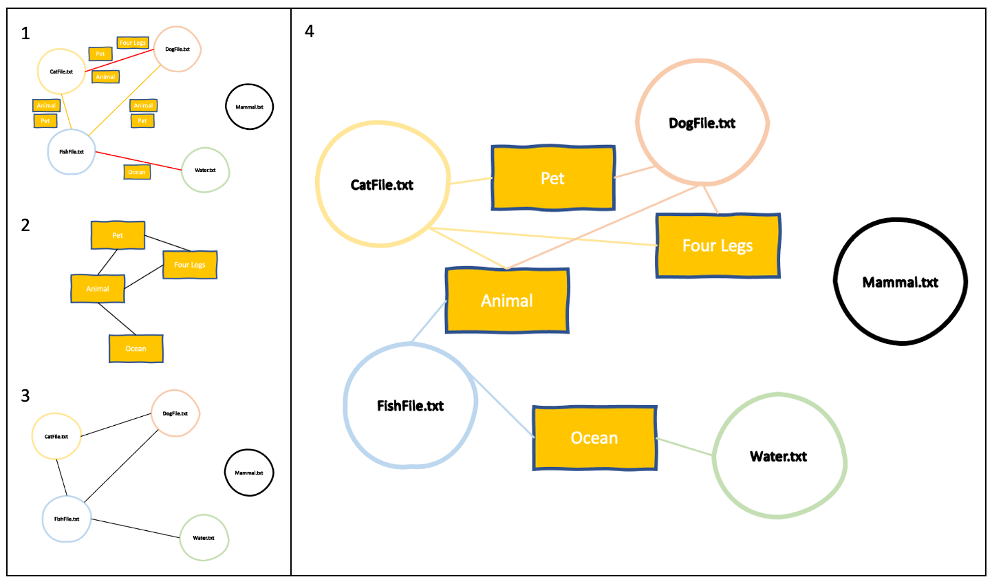
\includegraphics[width=1\textwidth]{images/wireframe.png}
  \caption{The development of initial wire frame of the Atlas web demonstrated the connections between documents with common keywords. The author experimented with different designs before settling on the circled document, boxed keyword arrangement (4).}
    \label{fig:wireframe}
\end{figure}

\begin{table}[!t]
\centering
\caption{The functional requirements and use cases that defined the minimum viable product.}
\label{tab:my-table}
\resizebox{\textwidth}{!}{%
\begin{tabular}{|l|l|p{4.5cm}|p{3cm}|p{6cm}|}
\hline
\textbf{Phase} & \textbf{Id} & \textbf{Functional Requirement} & \textbf{Use Case} & \textbf{Use Case Description} \\ \hline
\textbf{MVP} & F1 & To   form relationships between tagged words & Calculate   keyword links & When   the system is provided with a file system directory, it must parse the file contents and   calculate the Atlas Web. \\ \hline
\textbf{MVP} & F2 & To   display relationships on the user interface & Display   Atlas web & A   user should be able to view the Atlas Web that displays all of the files and   the relationships between them. \\ \hline
\end{tabular}%
}
\end{table}

Before developing Atlas, the author explored the requirements in greater detail with the aid of use cases and use case descriptions. Use case descriptions illustrate the behaviour of a system, without specifying how they are implemented (Hoda et al., 2008). On each iteration of the application, the author defined the use case descriptions for new functional requirements to help envision the technical implementation of the new features (Tables 3-6).

The author successfully implemented the initial functional requirements for the MVP (Figure ~\ref{fig:mvp}). Note, on seeing the user interface, they decided to use circles instead of squares to make the graph appear less complex. 

\clearpage
\begin{figure}[t!]
  \centering
      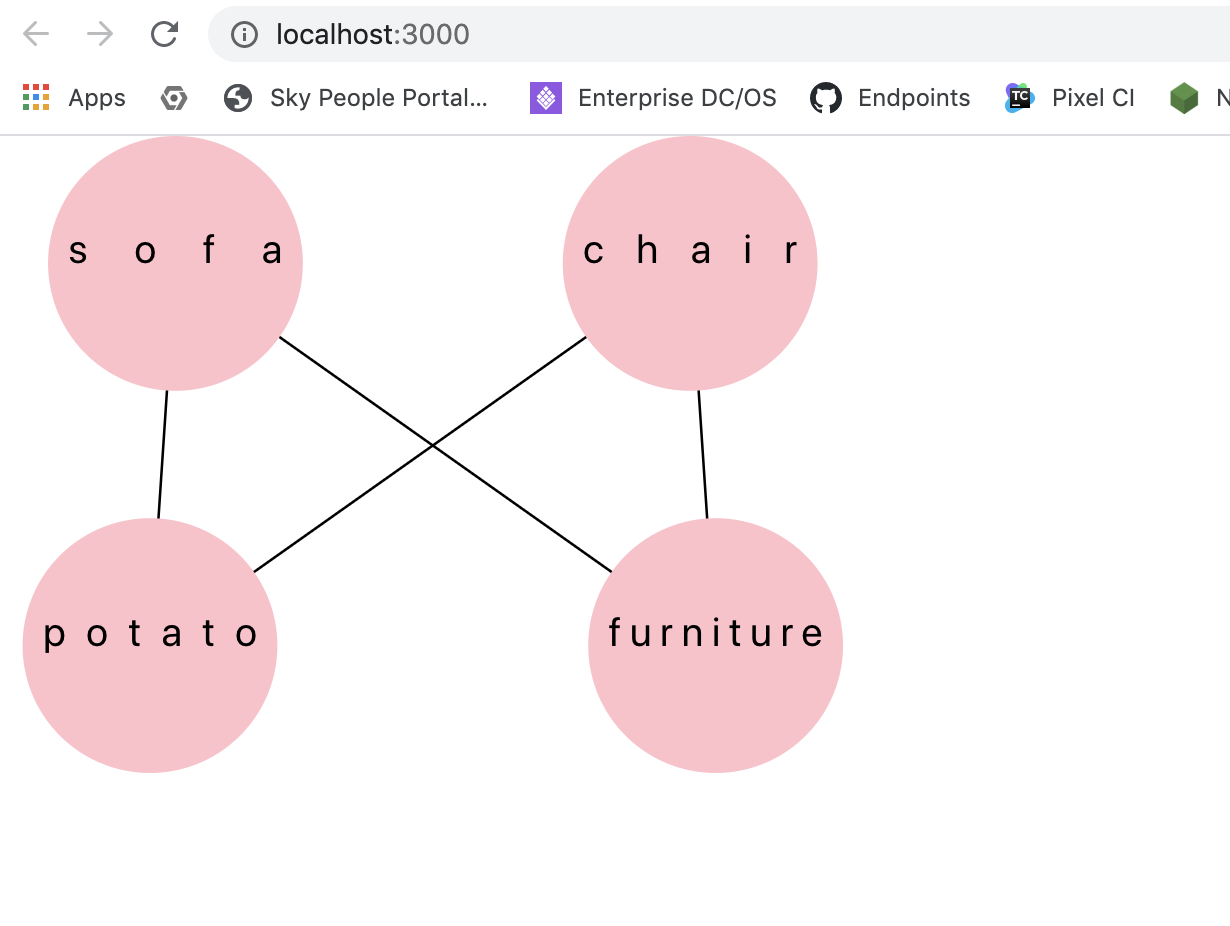
\includegraphics[width=1\textwidth]{images/mvp-frontend.png}
  \caption{The user interface of the Atlas MVP demonstrated the application ability to connect documents based on common tokenized keywords.}
  \vspace*{4in}
  \label{fig:mvp}
\end{figure}

\clearpage
\subsection{Iteration 2: Showcase and Survey}

To formulate the requirements used to iterate upon the MVP, the author showcased Atlas to members of their department. The presentation described the project aims and included a demonstration of the MVP Atlas Web (Figure ~\ref{fig:pres}). The dual purpose of the presentation was to inform colleagues of the author's apprenticeship work, and to collect feedback on the MVP. The presentation was followed by a survey which would inform the author of the success of implemented requirements and influence the development and prioritisation of future requirements. Due to Covid-19 restrictions, the showcase was held on Microsoft Teams with an audience of 15 members of the author’s organisation. 

\begin{figure}[!htb]
  \centering
      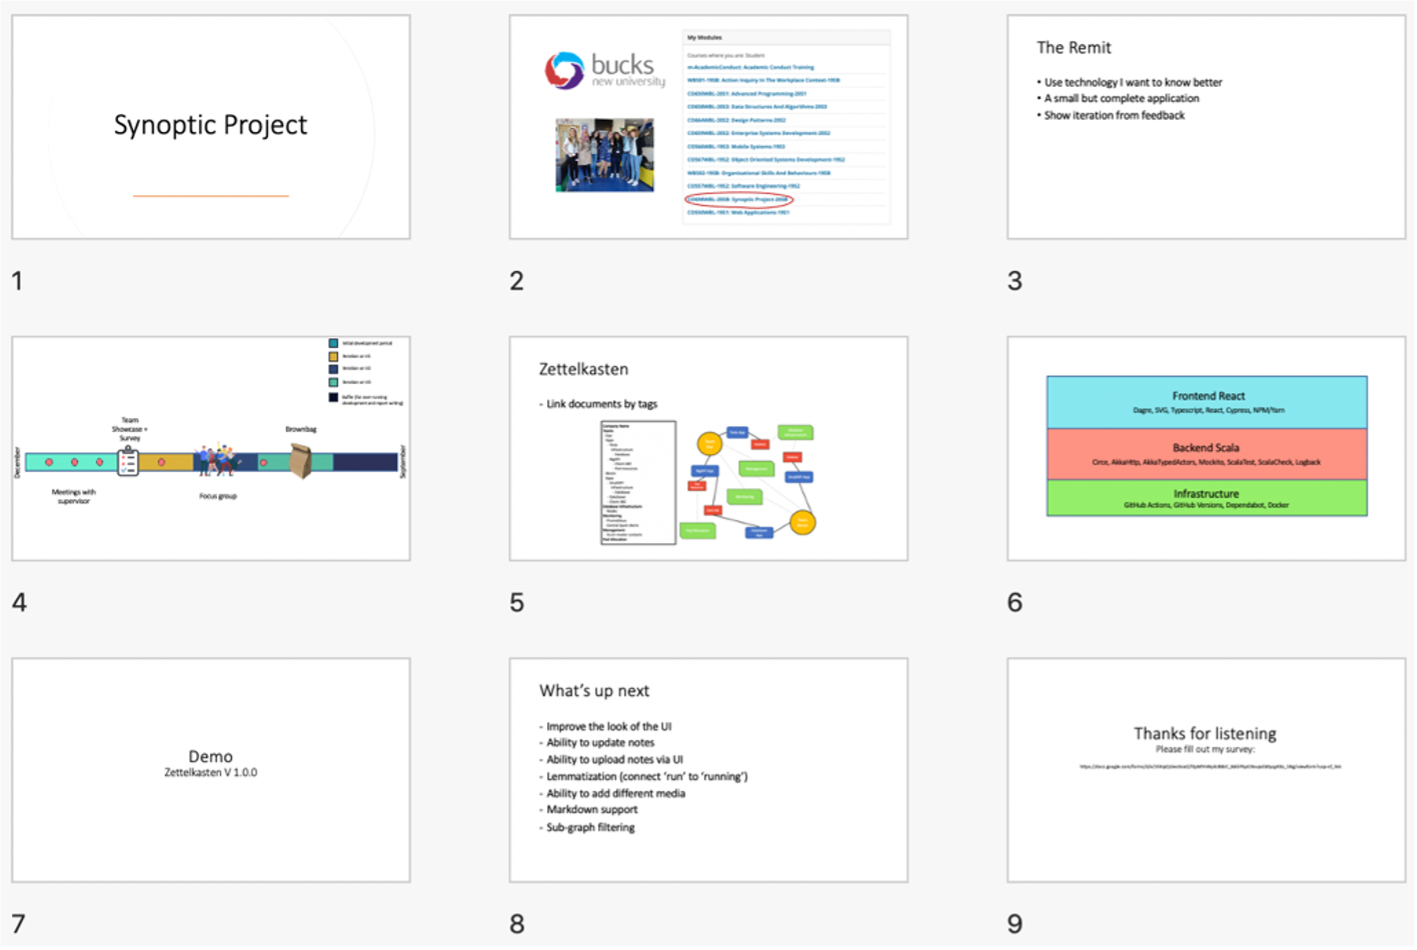
\includegraphics[width=1\textwidth]{images/showcase.png}
  \caption{The slideshow presentation showcased the project background and the MVP  to prospective users.}
  \label{fig:pres}
\end{figure}

The author purposely chose to showcase the MVP to members of the department early in the development process to generate an awareness of the project to the department. The author hoped this could lead to opportunities to collaborate with members of the department and could help find a team to maintain the application on completion. A stratified sample of 25 members of the department were invited to the showcase, but unfortunately 10 members could not attend. The demographic of the audience was largely male (80\%) and consisted of employees in technical roles. The author was aware that this population may not be reflective of the final user base, and could show a bias toward both male and technical opinions. This limitation was reflective of their departments population. However, the author noted if the product was to be utilised in the organisation, this would likely be the demographic that utilised the product.

After the showcase, attendees were asked to complete a survey (\hyperref[sec:appendix-1]{Appendix 1}). The survey offered a low cost and convenient mechanism for generating a large amount of data (Jones et al., 2013). It had two key purposes – the first was to understand whether the audience had understood the purpose of the current MVP concept, and the second was to give the opportunity to suggest future features. The survey contained primarily closed questions used to collect quantitative data on topics such as the user interface, the user journey and the users desire to user the application. Open questions enabled the respondents to suggest new features that the author may not have previously considered. The data was compiled and analysed to influence the priority of the next functional requirements (Figure ~\ref{fig:survey}).

The data analysis revealed that current MVP concept was well understood; as the average audience member rated product comprehension at a 7.9, user interface comprehension at  9.1 and user journey comprehension at 8.8. The audiences rated their likeliness to use the product as 7.1. Comments from the survey suggested this lower value may stem from concerns that the Atlas Web may not be able to handle larger document structures than demonstrated. The author ensured to demonstrate an Atlas Web with more documents in the future. Comments on the current MVP design also highlighted the fact that Atlas web was not centralised.

The survey prompted users to vote for Atlas’s upcoming features. By far, the most voted for new feature was the ability to open the documents within the application (F3). The second, third and fourth most voted features were the ability to add (F4), delete (F5) and edit (F6) documents. These formed the next four functional requirements for Atlas (Table 4).

\begin{figure}[!htb]
  \centering
      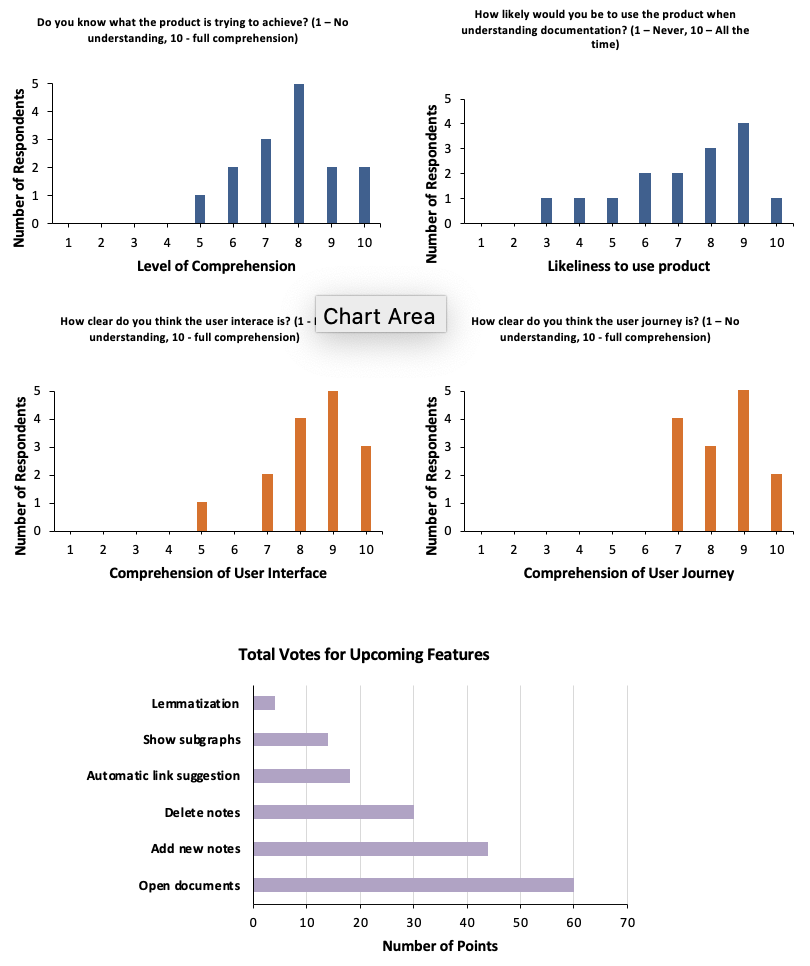
\includegraphics[width=1\textwidth]{images/survey-results.png}
  \caption{The minimal viable product survey revealed users comprehension of the current product and future features that they would like to see implemented.}
  \label{fig:survey}
\end{figure}
\clearpage

Interestingly, three survey respondents suggested the same additional feature – the ability to zoom in on the Atlas web interface. This ability proved more popular than the author’s suggested sub-graph feature. Although this feature was not incorporated into the second iteration of Atlas due to workload, the author highlighted this as a potential feature in the upcoming focus group.

\begin{table}[]
\centering
\caption{The functional requirements and use cases that defined the second iteration of Atlas.}
\label{tab:my-table}
\resizebox{\textwidth}{!}{%
\begin{tabular}{|l|l|p{4.5cm}|p{3cm}|p{6cm}|}
\hline
\textbf{Phase} & \textbf{Id} & \textbf{Functional Requirement} & \textbf{Use Case} & \textbf{Use Case Description} \\ \hline
\textbf{It. 2} & F3 & To   view document content & View   document content & A   user should be able to click on an Atlas web document to open a modal which   will display the document contents. \\ \hline
\textbf{It. 2} & F4 & To   add a new document & Add   a document & A   user should be able to add a new document to the Atlas Web. \\ \hline
\textbf{It. 2} & F5 & To   delete an existing document & Delete a document & A   user should be able to delete an existing documents from the Atlas Web. \\ \hline
\textbf{It. 2} & F6 & To edit  document content in the Atlas Web & Edit  a document & A   user should be able to edit a document to update the content. \\ \hline
\end{tabular}%
}
\end{table}

To aid the development of the second iteration, the author introduced a basic user actor to the system (Figure ~\ref{fig:user}). Atlas only catered to a single actor, as the primary purpose of the application was to automatically transform the file system into the Atlas web. As there was no concept of an admin user, all of the functionalities were carried out by the basic user.

\begin{figure}[!htb]
  \centering
      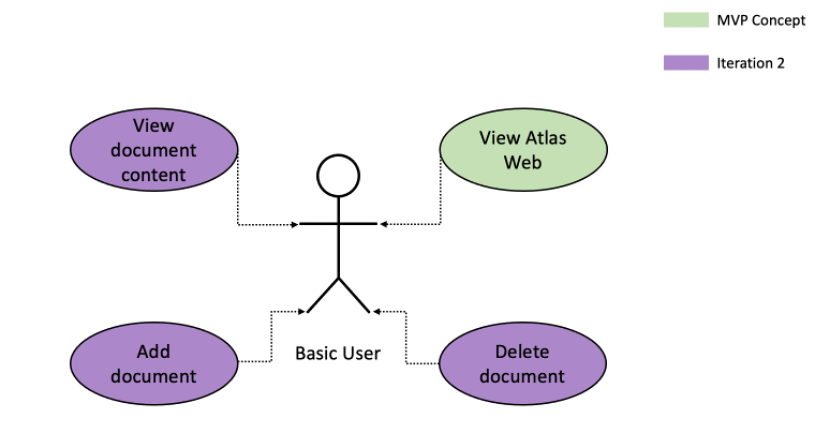
\includegraphics[width=1\textwidth]{images/actor-diagram.png}
  \caption{Actor diagram showing the new functionalities carried out by the user in the second iteration of Atlas.}
  \label{fig:user}
\end{figure}

\newpage

\subsection{Modal and Atlas Web Design}

Before the implementation of iteration 2 of Atlas, the author created wire frames to show the modal layout that will display document content. The wireframe provided a visual guide for the developer that ensured the element positions were both appealing and clear (Stone et al., 2005). The author also used the wireframes to update the design of the Atlas Web based on feedback from the survey.

The Atlas Web represented both documents and keywords as circles. As circles are universally known as clickable buttons, they enticed  users to interact with them. Relationship between the files were represented by lines. Lines were chosen over arrows, as not to overcrowd the screen or make the system appear overly complex by adding directionality to the relationships (Najjar, 1998). A user can add a new document by pressing the New File button on the Atlas Web user interface (Figure ~\ref{fig:modal}A). 

\begin{figure}[!htb]
  \centering
      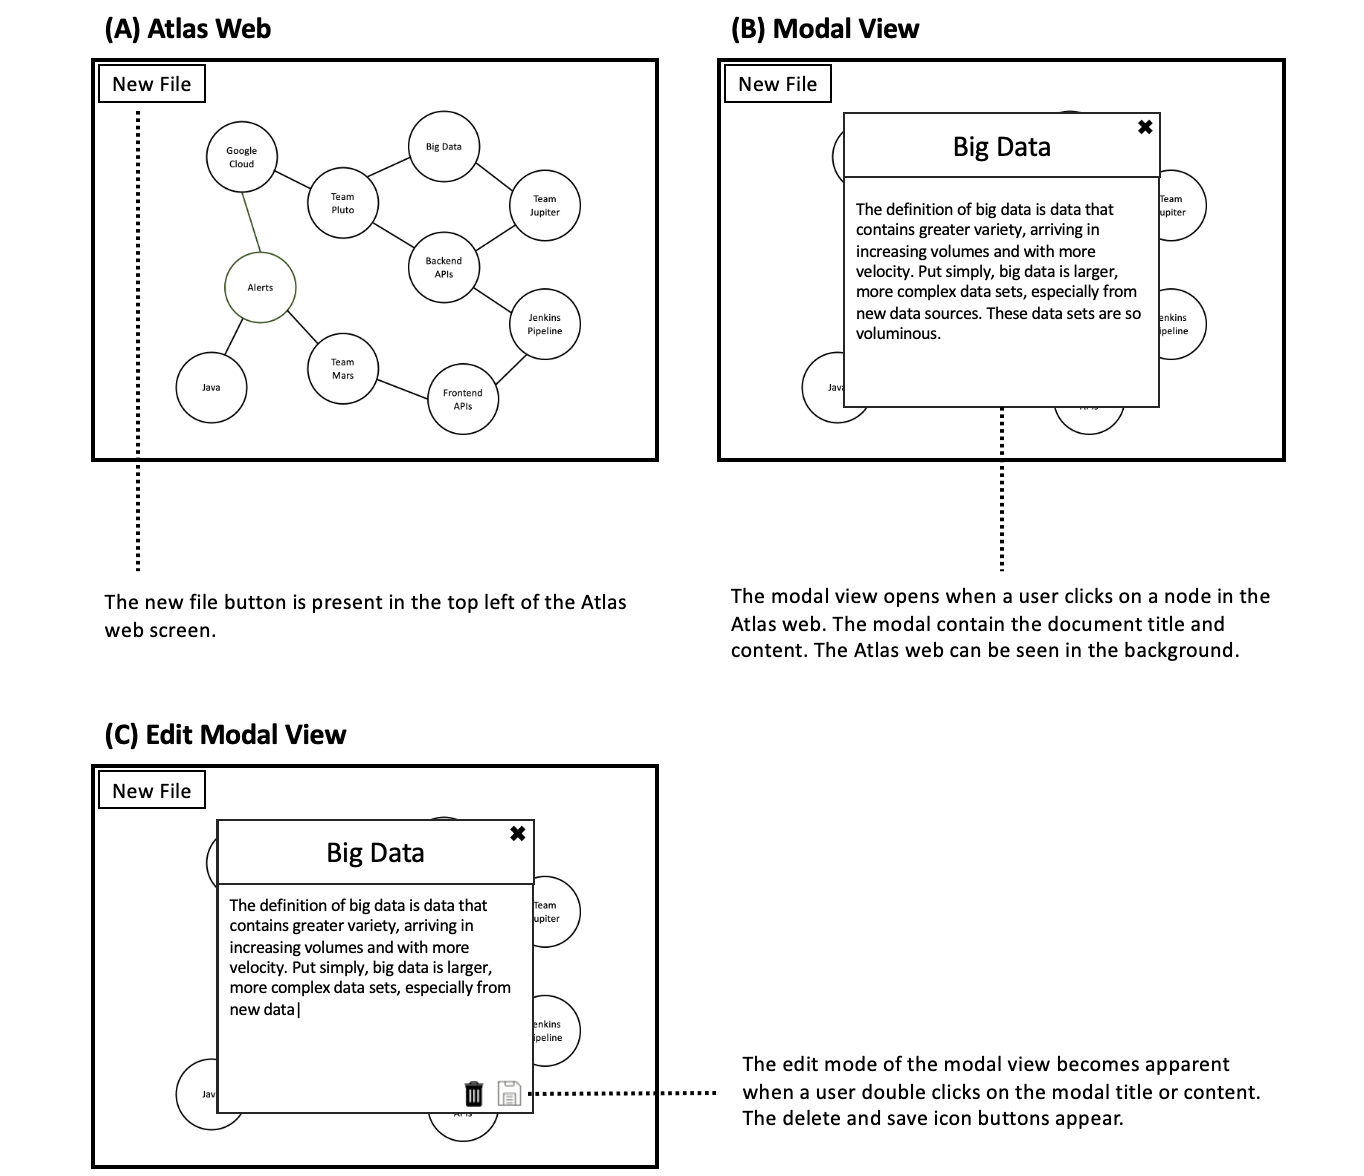
\includegraphics[width=1\textwidth]{images/modal-diagram.png}
  \caption{Wireframes representing the Atlas Web (A), the modal view (B), the edit modal view (C).}
  \label{fig:modal}
\end{figure}


When a user clicked the circular document button, a modal appeared with the document contents (Figure ~\ref{fig:modal}B). The appearance of a modal was chosen, rather than a new page, as it provided a smoother transition. The user could easily click on the background Atlas Web or the closing ‘X’ to close the modal. Therefore the user should feel confident navigating the product and should not feel lost between windows. Furthermore, the modal was chosen as it provided a distinct experience from the traditional file system which opens different files in different application windows.

The author decided to keep the design of the application simple and enable the user to both edit and delete the document within the modal view (Figure ~\ref{fig:modal}C). To edit a document, the user clicked the body or title of the modal. This mobile-centric approach was taken as it reduced the number of buttons on the user interface. The save and delete icons enable the user to update the document accordingly.

The author completed the development of the modal, and managed to produce a design similar to the intended wire frames (Figure ~\ref{fig:new-file}).

\begin{figure}[!htb]
  \centering
      \includegraphics[width=1\textwidth]{images/new-file.png}
  \caption{A user clicked on a document node in the Atlas Web to open the modal displaying the document content. Here the user is editing the document body.}
  \label{fig:new-file}
\end{figure}

\subsection{Iteration 3: Focus Group}

Once the second iteration of Atlas had been developed, further requirements were gathered with feedback from a focus group. The aim of the focus group was to gather different feelings and perspectives on the product (Gibbs, 1997). The focus group consisted of 6 members of the organisation, and included a small introduction to the product, followed by a demonstration that enabled users to interact with Atlas. Each user was encouraged to interact with the application so that they experienced all elements of the user journey. The author made note of any comments or concerns with the user experience (\hyperref[sec:appendix-1]{Appendix 1}). To ensure the focus group was reflective of the user base, a stratified sample of users across the organisation was selected, to incorporate a broader career range and a balanced gender ratio. 

The resulting qualitative data was analysed to find common sticking points with the application. Three members of the group initially struggled to understand how the application translated the traditional file system into the Atlas Web. It was suggested an instruction guide could alleviate this issue (F7). Furthermore, the focus group reported it was difficult to comprehend the Atlas Web when it had more than 15 nodes. The group responded positively to the author's suggestion of a zoom feature to help alleviate this issue (F8). Finally, on member of the group asked for the ability for Atlas to automatically recommend new connections if documents contained similar content (F9). The author prioritised these three new functional requirements by ease of implementation as they were aware of time constraints (Table 5).

\begin{table}[!h]
\centering
\caption{The functional requirements and use case descriptions that defined the third iteration of Atlas.}
\label{tab:my-table}
\resizebox{\textwidth}{!}{%
\begin{tabular}{|l|l|p{4.5cm}|p{3.2cm}|p{6cm}|}
\hline
\textbf{Phase} & \textbf{Id} & \textbf{Functional Requirement} & \textbf{Use Case} & \textbf{Use Case Description} \\ \hline
\textbf{It. 3} & F7 & To display an instruction guide & Display instructions & A user should be able to see the instruction guide when they first open the   application. \\ \hline
\textbf{It. 3} & F8 & To zoom into the Atlas Web & Zoom into Atlas web & A user should be able to zoom into different parts of the Atlas Web. \\ \hline
\textbf{It. 3} & F9 & To automatically suggest new connections & Suggest new document relationships & The system must be able to suggest potential connection based on common words. \\ \hline
\end{tabular}%
}
\end{table}

An unexpected development that stemmed from the focus group was the change of the products name. Originally, the product had been named ‘Zettelkasten’, after the author of the underlying transformation algorithm. The focus group reported the name had complex connotations and did not describe the product purpose well. For the fourth iteration of development, the author renamed the product to Atlas, as it was simpler and better aligned with the products purpose – the creation of knowledge maps.

The author successfully implemented the instruction guide (Figure ~\ref{fig:help}) and the zoom functionality (Figure ~\ref{fig:zoom}) and presented these features in the next iteration of development.

\begin{figure}[!htb]
  \centering
      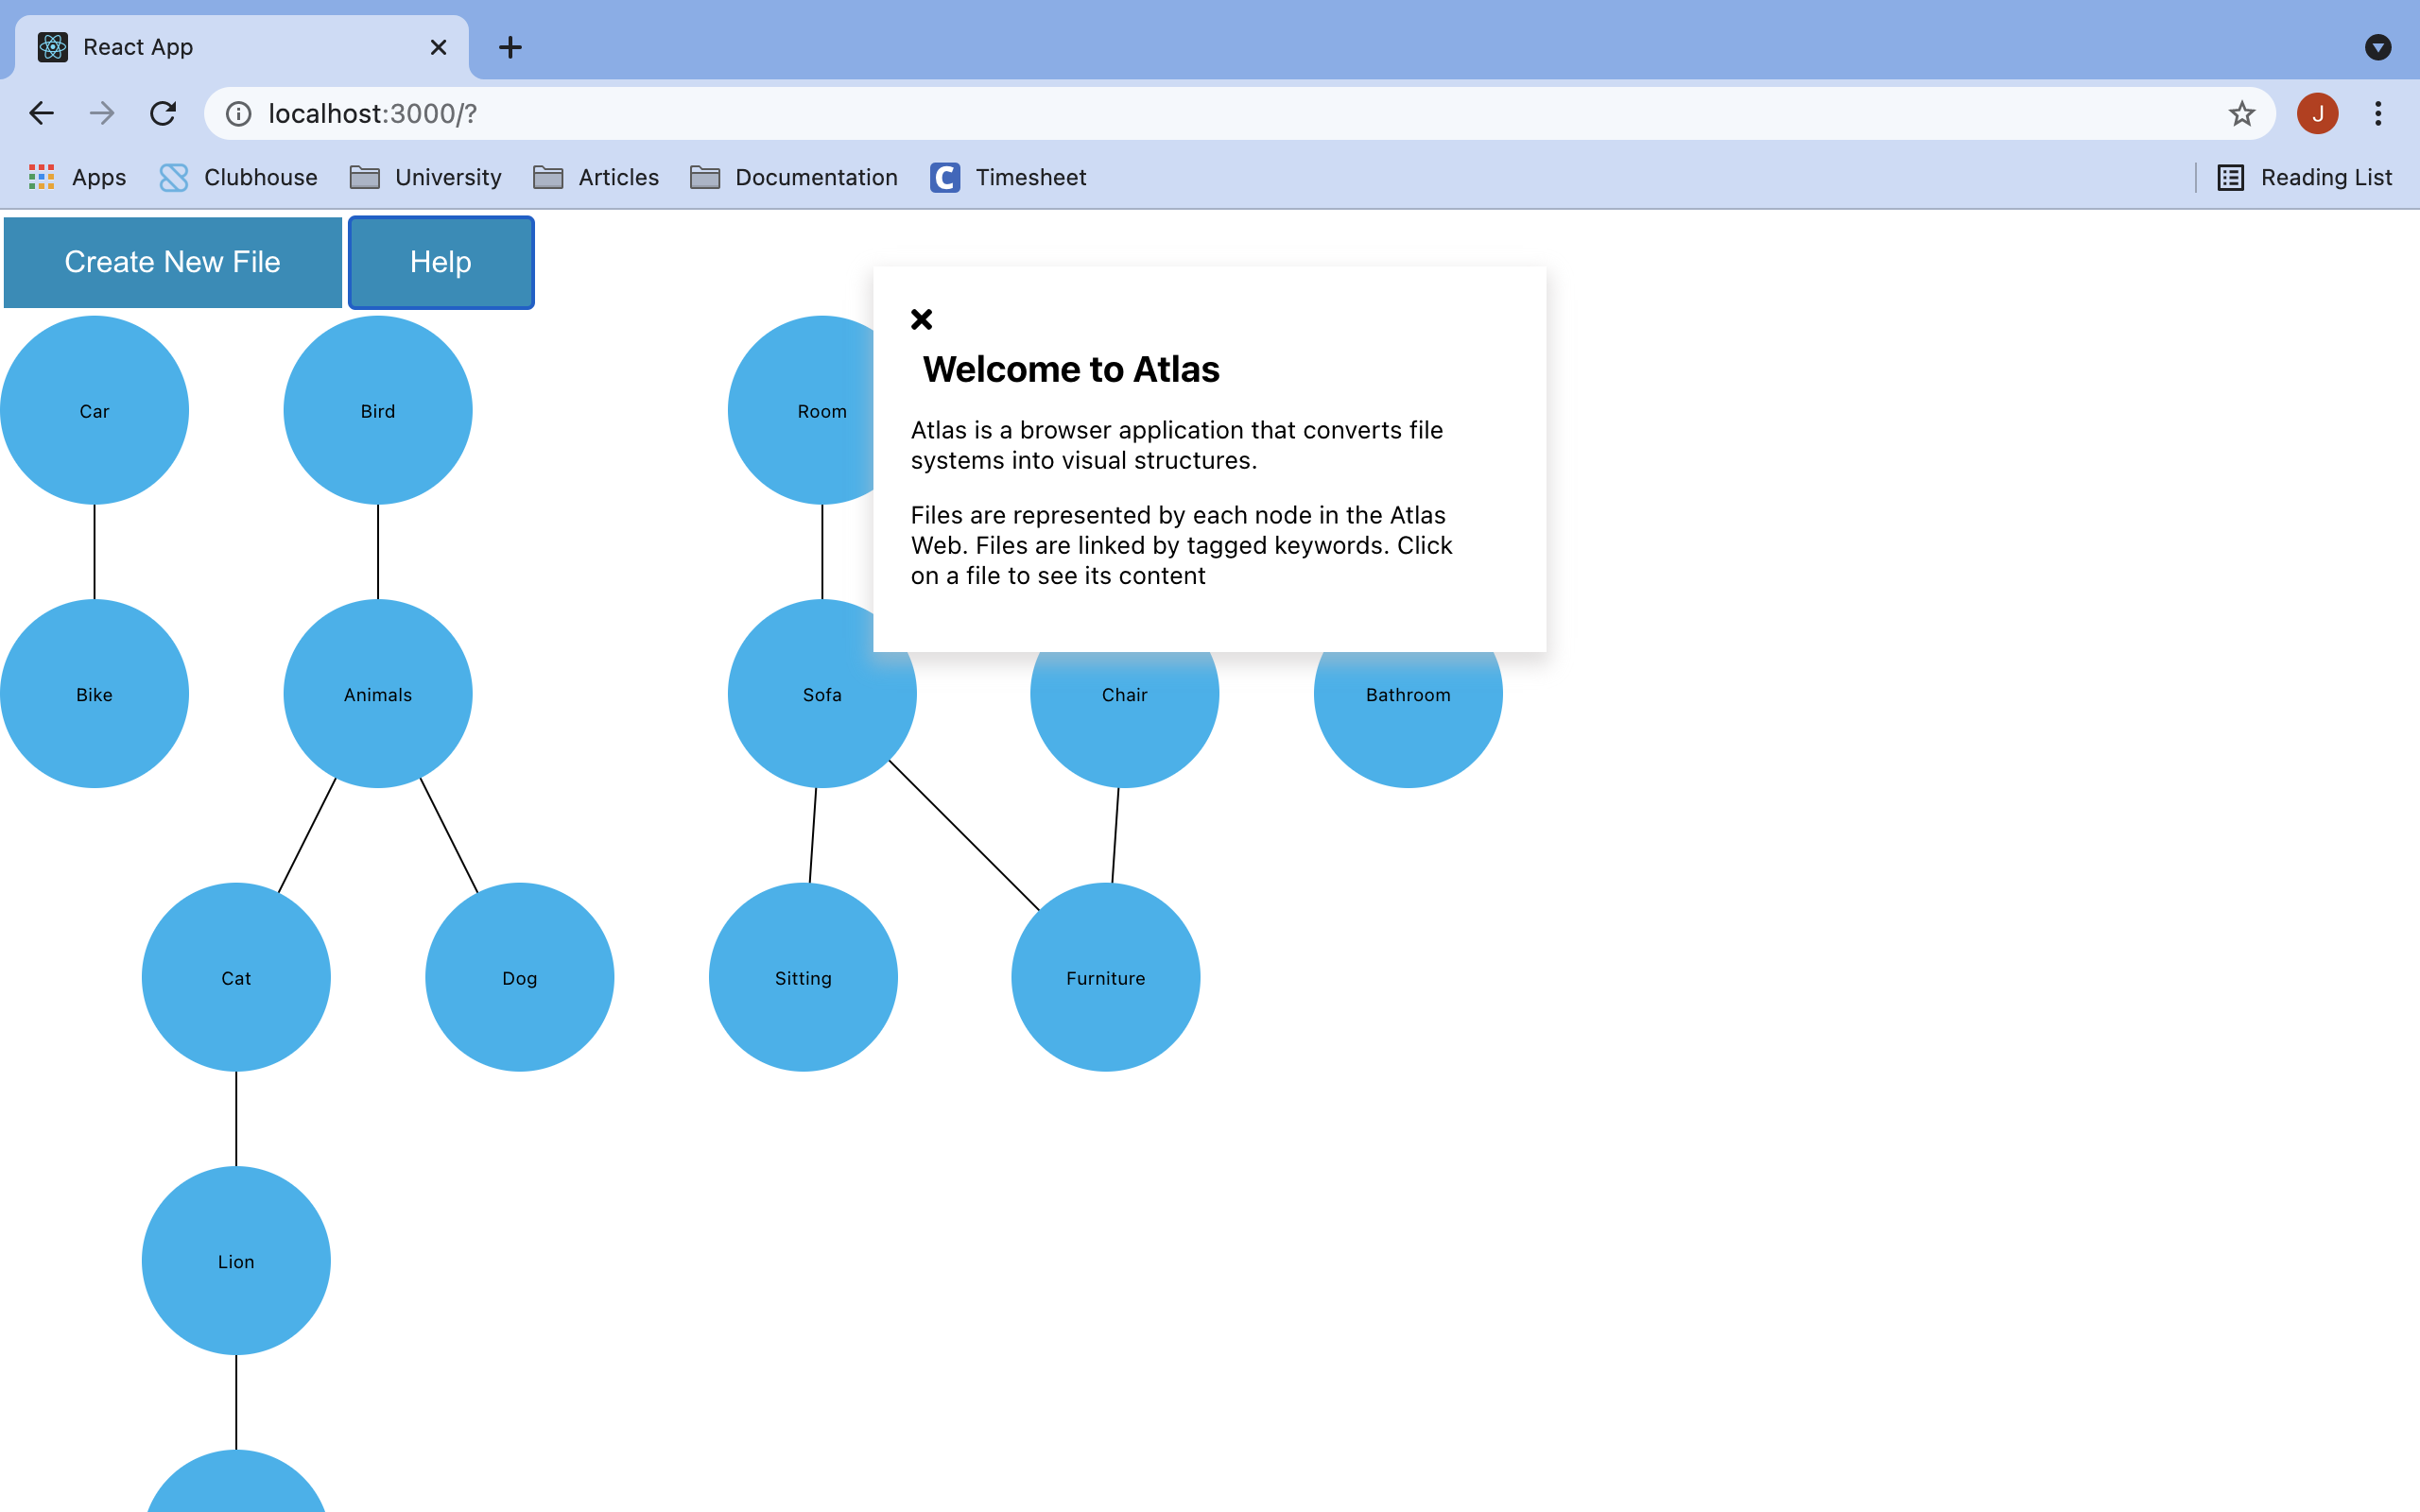
\includegraphics[width=1\textwidth]{images/help.png}
  \caption{By pressing the Help button, a user can open the instruction manual to instruct them on how to use Atlas.}
  \label{fig:help}
\end{figure}


\begin{figure}[!htb]
  \centering
      \includegraphics[width=1\textwidth]{images/zoom.png}
  \caption{The user can zoom into different parts of the Atlas Web using a touchpad drag and pinch or a mouse scroll.}
  \label{fig:zoom}
\end{figure}

\newpage
\subsection{Iteration 4: Interviews}

The author had planned to conduct interviews with several members of the organisation to gather more feedback and form more functional requirements. Interviews are particularly advantageous as the author is able to adapt their line of query to the interviewees responses (Gibbs, 1997). Unfortunately, the author only had time to informally interview one colleague, due to time restrictions. The feedback from the interview was largely positive. The interviewee suggested one additional feature - the ability to connect documents with similar names such as 'database' and 'databases' (Table 6). This process is known as stemming and had been previously researched by the author. The author successfully implemented the stemmer (Figure ~\ref{fig:before-after-stem}).

\begin{table}[!h]
\centering
\caption{The functional requirement and use case description that defined the fourth iteration of Atlas.}
\label{tab:my-table}
\resizebox{\textwidth}{!}{%
\begin{tabular}{|l|l|p{4.5cm}|p{4cm}|p{5cm}|}
\hline
\textbf{Phase} & \textbf{Id} & \textbf{Functional Requirement} & \textbf{Use Case} & \textbf{Use Case Description} \\ \hline
\textbf{It. 4} & F10 & To connect documents with the same stem & Connect documents with the same file name stems & The system must connect document with the same file name stems. \\ \hline
\end{tabular}%
}
\end{table}

\begin{figure}[!htb]
  \centering
      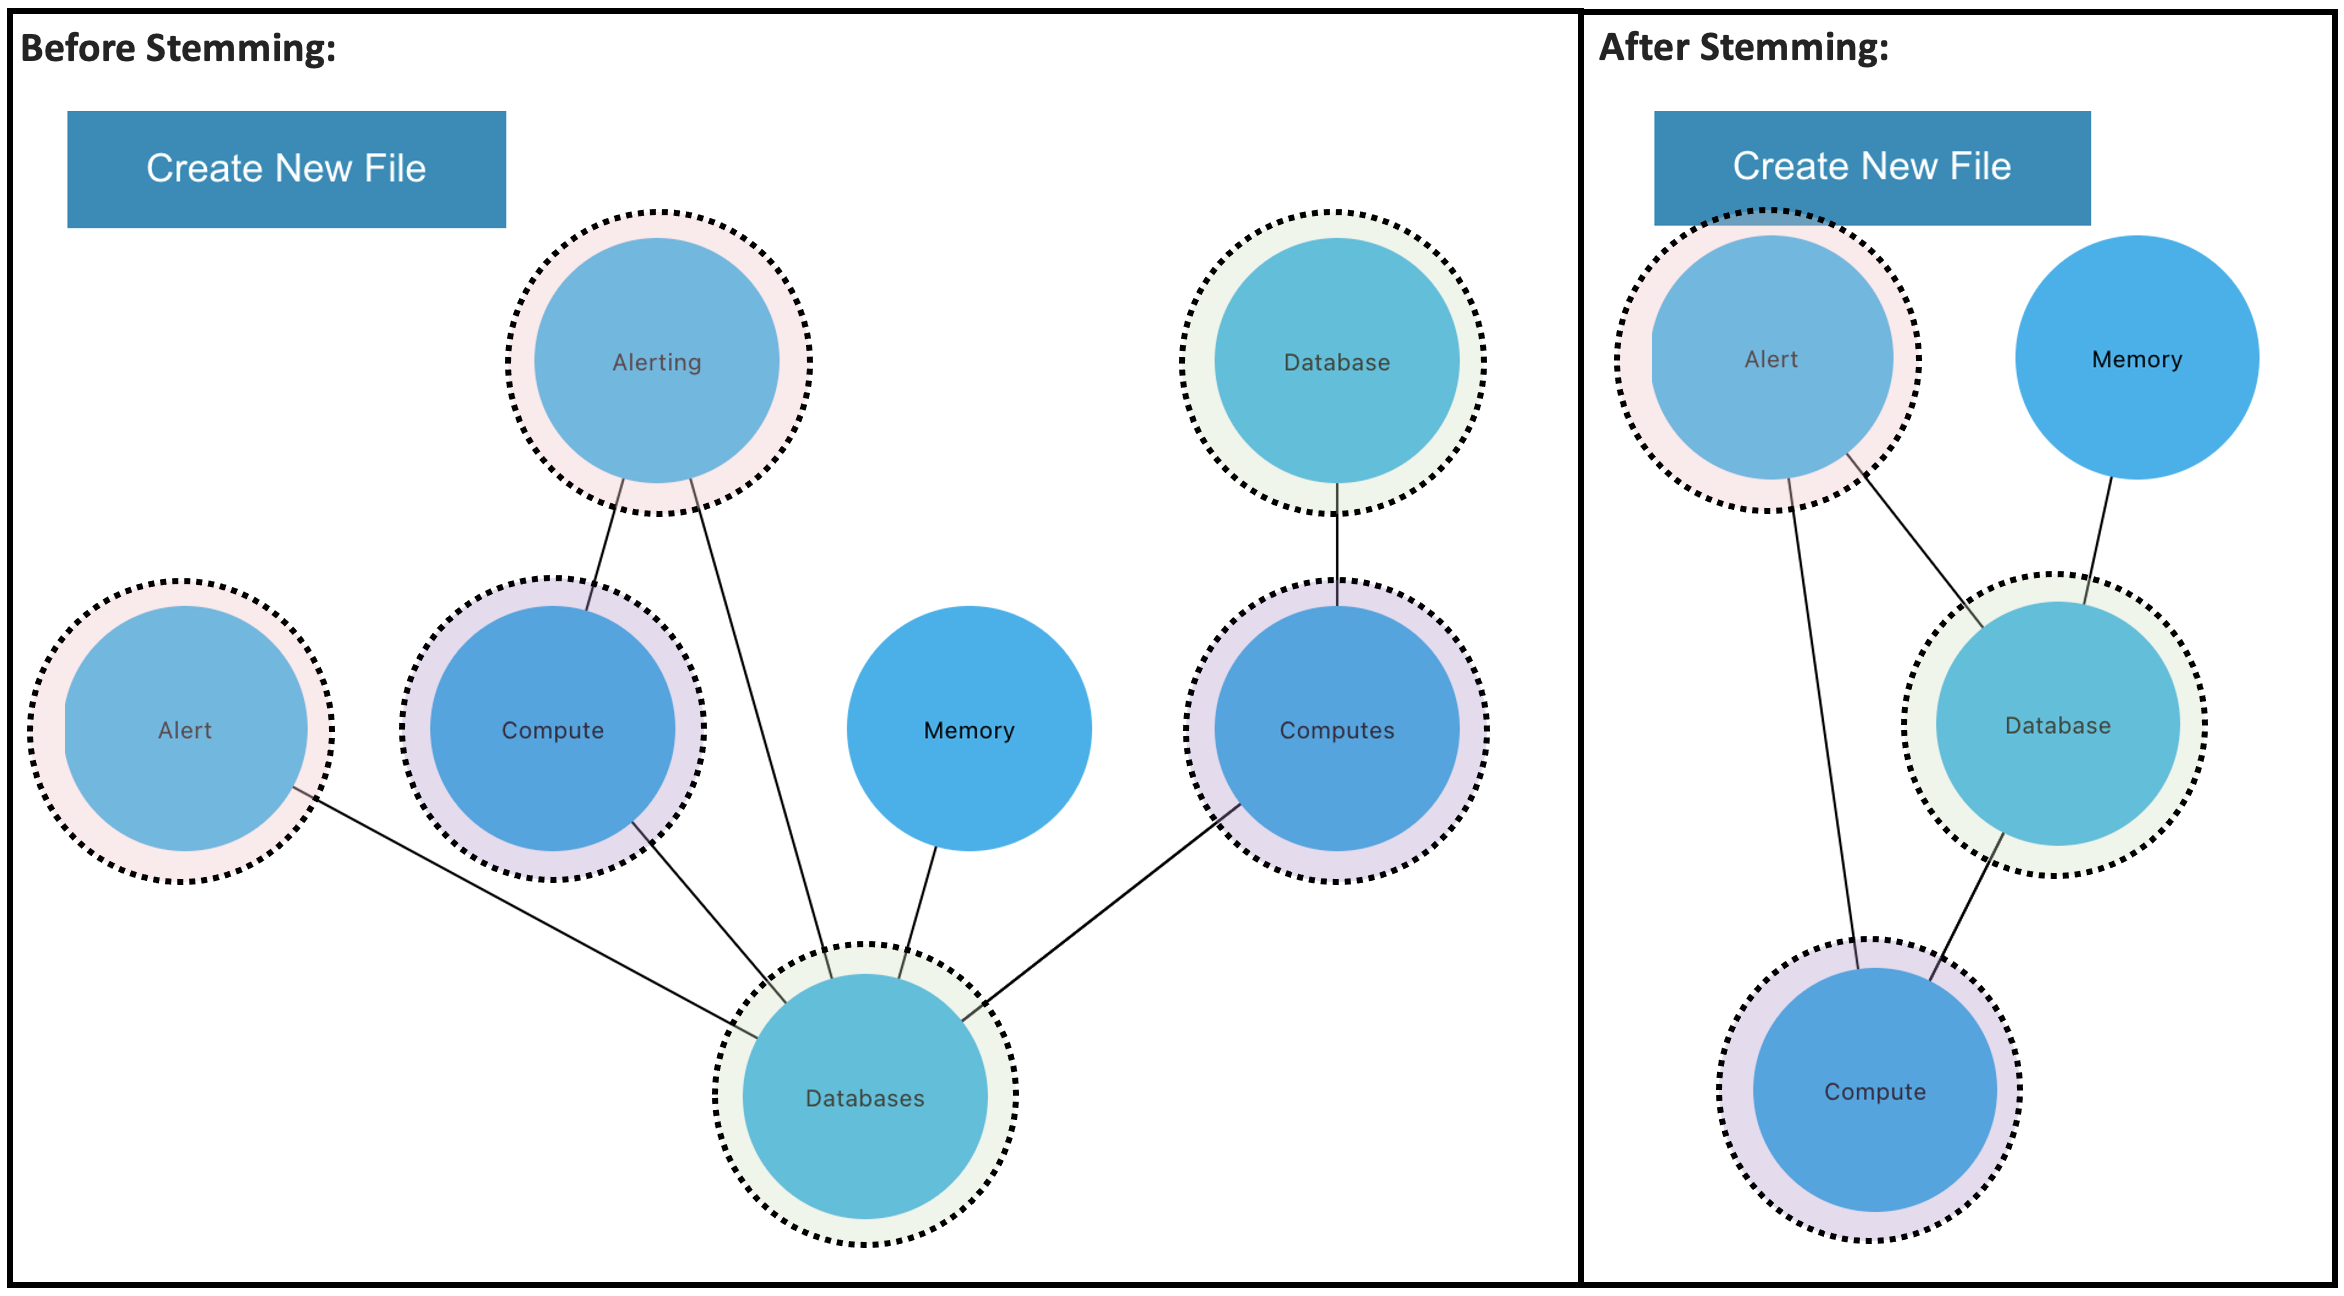
\includegraphics[width=1\textwidth]{images/before-after-stem.png}
  \caption{The author successfully implemented a stemmer to connect files with the same stem.}
  \label{fig:before-after-stem}
\end{figure}

In order to implement the stemming requirement (F10), the author used a sequence diagram to guide the implementation (Figure ~\ref{fig:seq}). Sequence diagrams demonstrate the interaction between systems over time (Fowler, 2003). This enabled the author to understand that when a user provided the location of a file system, the system could then identify the nodes and edges of the documents by parsing each file individually. The nodes would then be stemmed when they were identified by the system.

\begin{figure}[!htb]
  \centering
      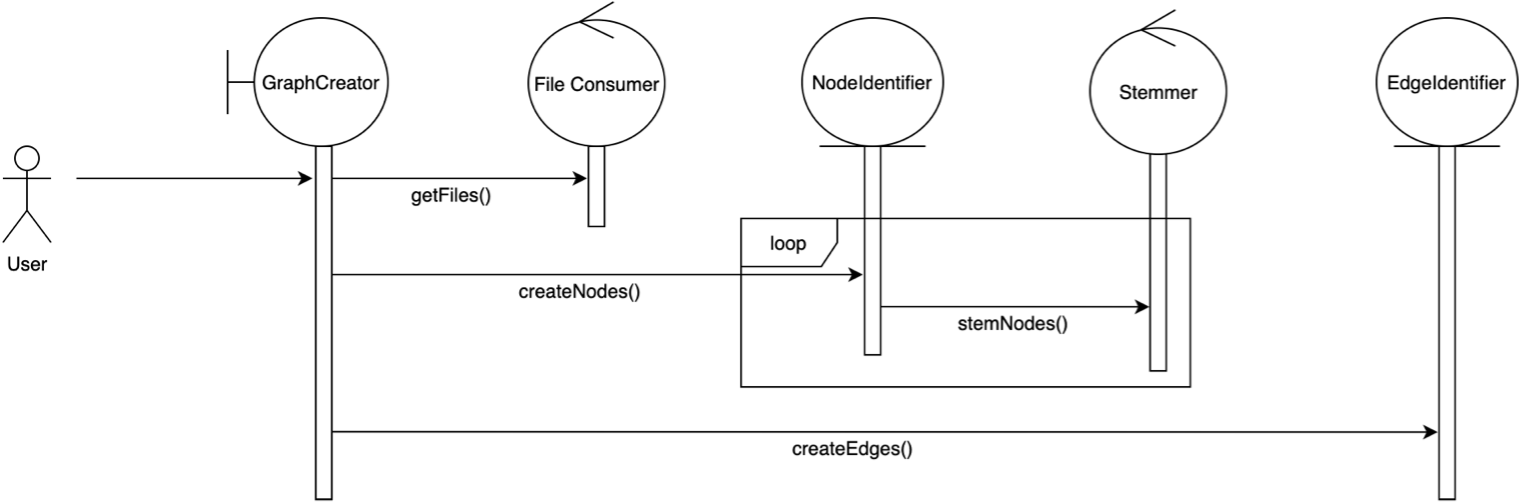
\includegraphics[width=1\textwidth]{images/sequence-diagram.png}
  \caption{The sequence diagram demonstrate how a user interacts with the system to create an Atlas web.}
  \label{fig:seq}
\end{figure}

\clearpage

\subsection{Class Diagram with Entity Relationships}

To translate the use case descriptions into a technical design, the author consolidated class diagrams with the entity relationships schemas to demonstrate the relationship between the classes and objects within the system (Figure ~\ref{fig:ent}). The author first created this diagram before the MVP concept was implemented, and extended it with each iteration of the application. The diagram was then used as a reference point to guide the development of Atlas.

The case class diagram shows two key packages – the file consumer package consisting of the FileConsumer trait and LocalFileConsumer class, and the GraphGenerator package consisting of eight objects and classes connected to the GraphCreator class. The GraphCreator class utilised the EdgeIdentifier and NodeIdentifier objects to produce the list of files and related nodes which in turn, generated the Graph displayed to the user. These objects were supported by the FilesAndTags class, with the resulting objects being combined by the GraphCreator. The NodeIdentifier object was further supported by the Stemmer object, which enabled the stemming functionality.

\begin{figure}[!htb]
  \centering
      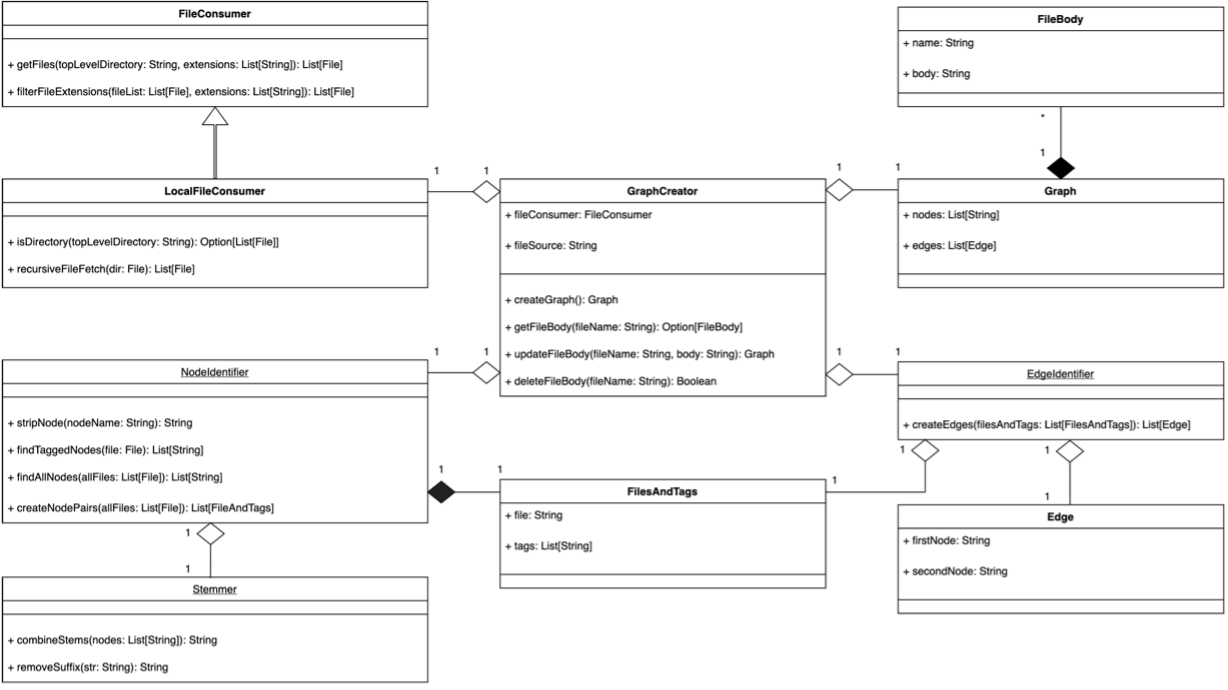
\includegraphics[width=1\textwidth]{images/entity-relationship.png}
  \caption{The combined case class and entity relationship diagram that guided the development of the Atlas system.}
  \label{fig:ent}
\end{figure}

\subsection{Non-Functional Requirements}

Whilst the functional requirements defined the behaviour of the application, the non-functional requirements described the system level attributes such as the performance, security, usability and reliability (Augustine et al., 2005). Non-functional requirements are important as they can determine whether the user has a positive user experience. The non-functional requirements of Atlas were solicited throughout the development process (Table 7). The focus group elicited the importance of the user’s ability to understand and comprehend the applications features (NF1). The second and third non-functional requirements concerned with the security (NF2) and speed (NF3) of the application and were influenced by the guidelines of similar applications (Addison-Wesley, 2003). The final non-functional requirement focused upon the developer experience (NF4). It was important to maintain a clean code base, as the application may have to be maintained by other members of the department. 

\begin{table}[!hb]
\footnotesize
\caption{The non-functional requirements of Atlas were solicited to provide a smooth user and developer experience.}
\centering
\label{tab:my-table}
\resizebox{\textwidth}{!}{%
\begin{tabular}{|l|p{6cm}|p{5cm}|}
\hline
\textbf{Id.} & \textbf{Non-Functional   Requirement} & \textbf{Example} \\ \hline
\textbf{NF1} & A user must be able to understand the Atlas   Web and be able to navigate the user interface with ease. & A user should be able to understand the application by reading the instructions. \\ \hline
\textbf{NF2} & The security of a system must keep user information confidential and prevent any unwanted outside   interaction with the system. & User data must only be stored locally. \\ \hline
\textbf{NF3} & The application performance must respond   rapidly to user requests. & A user should be able to see a newly added node appear on the user interface within 500ms\textsuperscript{-1}. \\ \hline
\textbf{NF4} & The   application codebase must be well maintained and accessible for future   developers. & A linter will be used to reduce the amount of   errors and stylistic differences. \\ \hline
\end{tabular}%
}
\end{table}

\newpage
\section{Development}
\subsection{Time Management}

A total of four iterations of Atlas were developed. The first iteration, the MVP, was completed as planned in early March after 14 weeks of development. The three later iterations of the application did not meet the initial schedule, as the first iteration overran by 3 weeks (Figure ~\ref{fig:github}). Time management problems were highlighted as a low risk in the initial product plan (R4) as a 20\% buffer had been added to all time estimates. Although all four iterations of the product were implemented, the author had significantly less time to write the project report than originally allocated.

\begin{figure}[!htb]
  \centering
      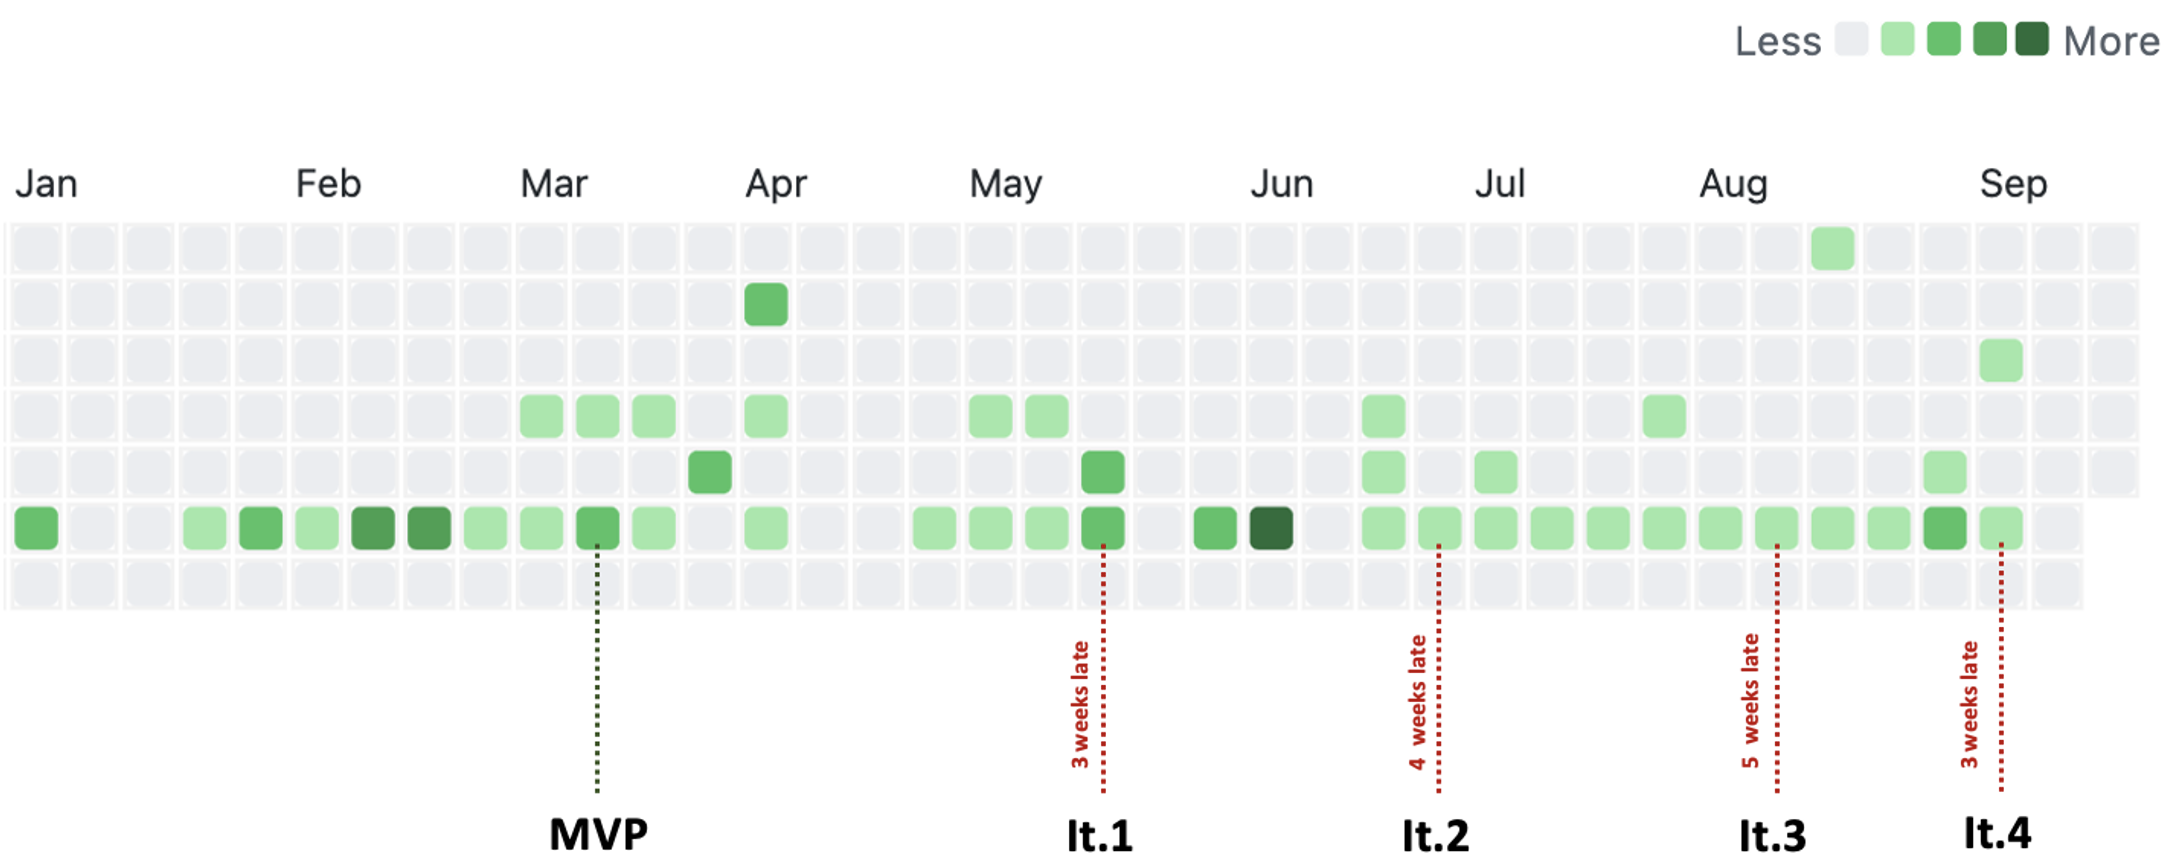
\includegraphics[width=1\textwidth]{images/timeline.png}
  \caption{Annotated GitHub commit chart demonstrates the successful completion of the MVP on schedule, followed by time slippage on the later iterations of Atlas.}
  \label{fig:github}
\end{figure}

The author had dedicated half a day per week to the project to allow time for work on parallel university modules. This assumption proved inaccurate, as the high time demands of the other modules resulted in little time for project development. Due to high work demands outside of the apprenticeship, the product could not be developed as part of the author's daily work. As a result, the author found themselves developing the project outside of the allocated hours, which in turn made it difficult to gain momentum on each iteration. Furthermore, the additional task of writing the report led to later stages of development becoming particularly rushed. Fortunately, the Scrumban agile methodology enabled the author to prioritise important tasks and omit those not required to create a functionally complete product.

\subsection{Completed Functionality}

The author implemented 9 of the 10 functional requirements outlined in the original requirements and design section (Table 8). The automatic tag suggestion requirement (F9) was omitted due to the aforementioned time constraints. The author struggled to develop a solution for automatic tag generation which could efficiently store and identify words common to multiple documents as the data set scales. If this requirement was further developed, the author would research Scala frameworks which could store and manipulate large quantities of data such as the Play Framework (PlayFramework, 2021).

\begin{table}[!hb]
\centering
\tiny
\caption{A list of the functional requirements included in the final iteration of Atlas.}
\label{tab:my-table}
\resizebox{\textwidth}{!}{%
\begin{tabular}{|l|p{9cm}|l|}
\hline
\textbf{Id} & \textbf{Functional Requirement} & \multicolumn{1}{l|}{\textbf{Completed?}} \\ \hline
\textbf{F1} & To form relationships between tagged words & \cellcolor[HTML]{92D050}\checkmark️ \\ \hline
\textbf{F2} & To display relationships on the user interface & \cellcolor[HTML]{92D050}\checkmark️ \\ \hline
\textbf{F3} & To view document content & \cellcolor[HTML]{92D050}\checkmark️ \\ \hline
\textbf{F4} & To add a new document & \cellcolor[HTML]{92D050}\checkmark️ \\ \hline
\textbf{F5} & To delete an existing document & \cellcolor[HTML]{92D050}\checkmark️ \\ \hline
\textbf{F6} & To edit an existing document & \cellcolor[HTML]{92D050}\checkmark️ \\ \hline
\textbf{F7} & To display the instruction guide & \cellcolor[HTML]{92D050}\checkmark️ \\ \hline
\textbf{F8} & To zoom into the Atlas Web & \cellcolor[HTML]{92D050}\checkmark \\ \hline
\textbf{F9} & To   automatically suggest new connections & 
\cellcolor[HTML]{EA5563}\\ \hline
\textbf{F10} & To   stem similar words & \cellcolor[HTML]{92D050}\checkmark \\ \hline
\end{tabular}%
}
\end{table}

\subsection{Completed Objectives}

The author implemented 3 of the 4 original objectives (Table 9). The author was satisfied that they had created a well-design product that could efficiently aid users with the transformation of a file system into an Atlas Web (O2). Furthermore, they believe that with the implementation of user feedback, they developed a product that clearly depicts the relationships between documents (O3 and O1). Although the code for Atlas is available on GitHub, the author did not deploy Atlas into a production environment due to the author not being able to have the resources to deploy the application into their department (O4). The author is awaiting to see it if Atlas will be maintained by the department.

\begin{table}[!h]
\centering
\small
\caption{A list of the objectives included in the final iteration of Atlas.}
\label{tab:my-table}
\resizebox{\textwidth}{!}{%
\begin{tabular}{|l|l|l|}
\hline
\textbf{Id} & \textbf{Objective} & \textbf{Completed?} \\ \hline
\textbf{O1} & Design a user interface that clearly depicts the   relationships between documentation. & \cellcolor[HTML]{92D050}\checkmark \\ \hline
\textbf{O2} & Develop a minimal viable product that can   transform a specified file system into the web interface. & \cellcolor[HTML]{92D050}\checkmark️ \\ \hline
\textbf{O3} & Gather and incorporate user feedback on the   minimal viable product and develop future iterations of the application. & \cellcolor[HTML]{92D050}\checkmark️ \\ \hline
\textbf{O4} &  Deploy Atlas into a production environment so that it can be used by organisation members. & \cellcolor[HTML]{FFC000} \\ \hline
\end{tabular}%
}
\end{table}

\newpage

\subsection{Spike: Front-end React Development}

During the development of the MVP, the author dedicated a day of development to a spike on front-end libraries. A spike is a method for evaluating the impact of new technology that enables the developer to become more confident with the desired approach (Agile Learning Labs, 2021). The author had highlighted their lack of experience with front-end development as a risk from the outset (R1), and as a result they wanted to explore different solutions for the visualisation of the Atlas Web. This exploration would also help the author minimise another  risk, the inability of the chosen technology to efficiently generate the Atlas web (R2).

The author explored two key solutions for front-end web generation. The first, was to create the Atlas Web with their own React components. From utilising online resources, the author had learnt that it was easy to create basic shape components in React such as the lines and circles which form the basis for the web. The author found shape manipulation in space to be difficult to calculate as the relative coordinates changed with screen size and scale (Figure ~\ref{fig:dagre}A). The second solution the author explored was the use of the Dagre library. Dagre is a JavaScript library that configures the position of elements in a graph (Pettitt et al., 2013). Using Dagre, the author could easily manipulate the Atlas Web layout (Figure ~\ref{fig:dagre}B). The author decided to implement Dagre as it provided an efficient bespoke layout engine for generating the Atlas Web. Choosing Dagre mitigated the risk of building a bloated code base as it encompassed the required positional calculations (R5).

\begin{figure}[!b]
  \centering
      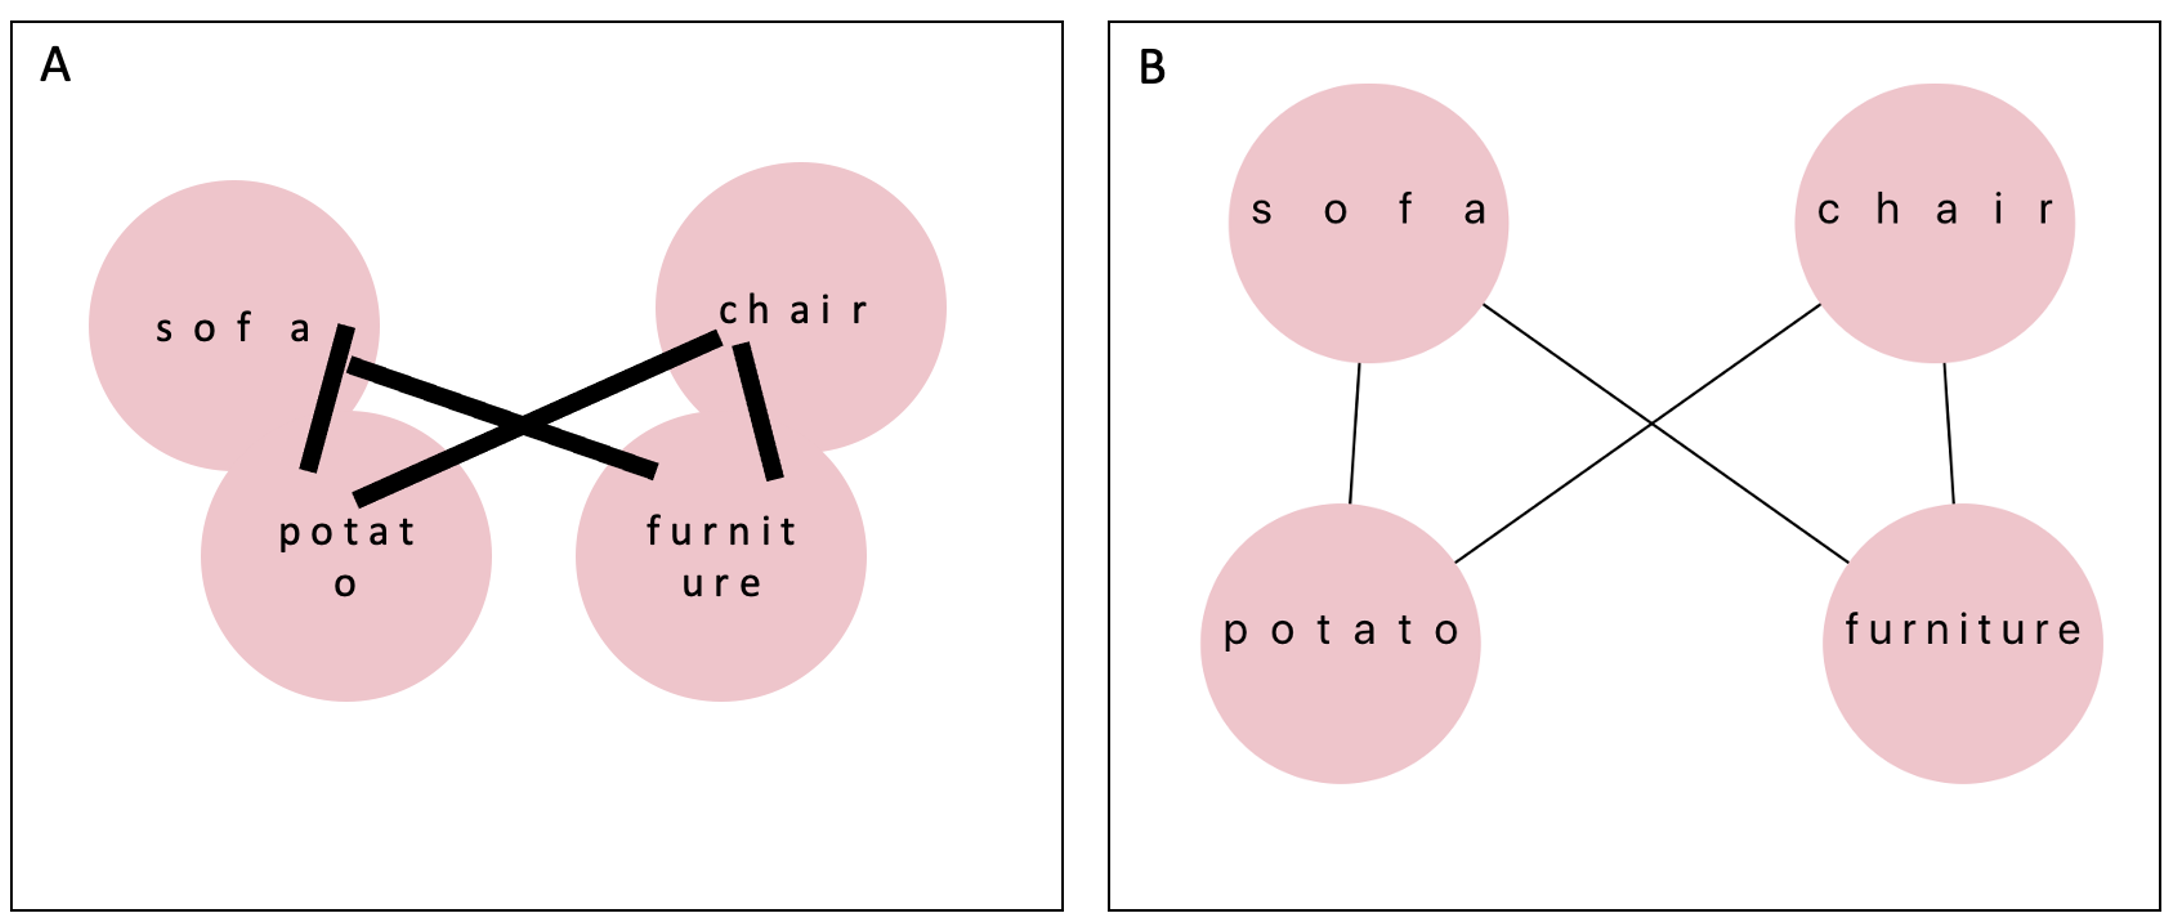
\includegraphics[width=1\textwidth]{images/dagre.png}
  \caption{The result of the front-end spike encouraged the author to use the front-end Dagre library (B) rather than create their own framework (A).}
  \label{fig:dagre}
\end{figure}

\newpage

\subsection{Technical Challenge: Porter Stemmer Algorithm Implementation}

In order to link nodes with the same stem in the Atlas Web, the author incorporated the Porter algorithm. The Porter algorithm removes a suffix from a word to obtain the stem (Porter, 1980). For example, words such as ‘makes’, ‘make’ and ‘making’ will be reduced to ‘make’ after stemming. The Porter algorithm enabled different inflections of the same word become linked in the Atlas Web.

There are three predominant stemming algorithms found in natural language processing: the Porter algorithm (Porter, 1980), the Snowball algorithm (Porter, 2001), and the Lancaster algorithm (Paice, 1990). The Porter algorithm is less complex than the Snowball and Lancaster algorithms, and often produces more intuitive representations of stemmed words. Although, the Porter algorithm is slightly less performant than the Lancaster algorithm (Porter, 2001), as the author saw no latency increases in Atlas Web generation, they chose the Porter implementation. Note, this algorithm is appropriate for other languages, enabling this feature to be used in the author's global organisation (Porter, 1980).

The implementation of the Porter algorithm incorporated rules such as the pattern of consonants and vowels, and the letters in the stem (Figure ~\ref{fig:porter}). The algorithm was particularly challenging, as the author had to manipulate the characters in the file name to calculate the measure of the consonants and vowels, in addition to identifying any rule triggering suffixes. There were no Scala examples of the Porter algorithm online, therefore, the author was challenged with developing a unique implementation.

\begin{figure}[!hb]
  \centering
      \includegraphics[width=1\textwidth]{images/porter-stemmer.png}
  \caption{The author implemented the rules of the Porter stemmer algorithm to standardise the file names.}
  \label{fig:porter}
\end{figure}

\clearpage

\subsection{Technical Challenge: CORS Handler Implementation}

During the local development of the MVP, the author was confronted with a communication issue between the front-end and the back-end of Atlas. Atlas was designed to be segregated to simplify the development between the two different areas and to enable respective scaling. However, the communication between the two was initially blocked by the presence of a Cross-Origin Resource Sharing (CORS) Policy error. CORS is a security mechanism in modern browsers that controls the access of resources from outside of the browser domain (Mozilla, 2021). When the author created the front-end server to invoke the back-end CRUD requests, they did not realise that CORS would invoke an OPTIONS security request before sending the intended CRUD call. As the back-end was not configured to handle the OPTIONS request, it resulted in a CORS policy error (Figure ~\ref{fig:cors}).

\begin{figure}[!h]
  \centering
      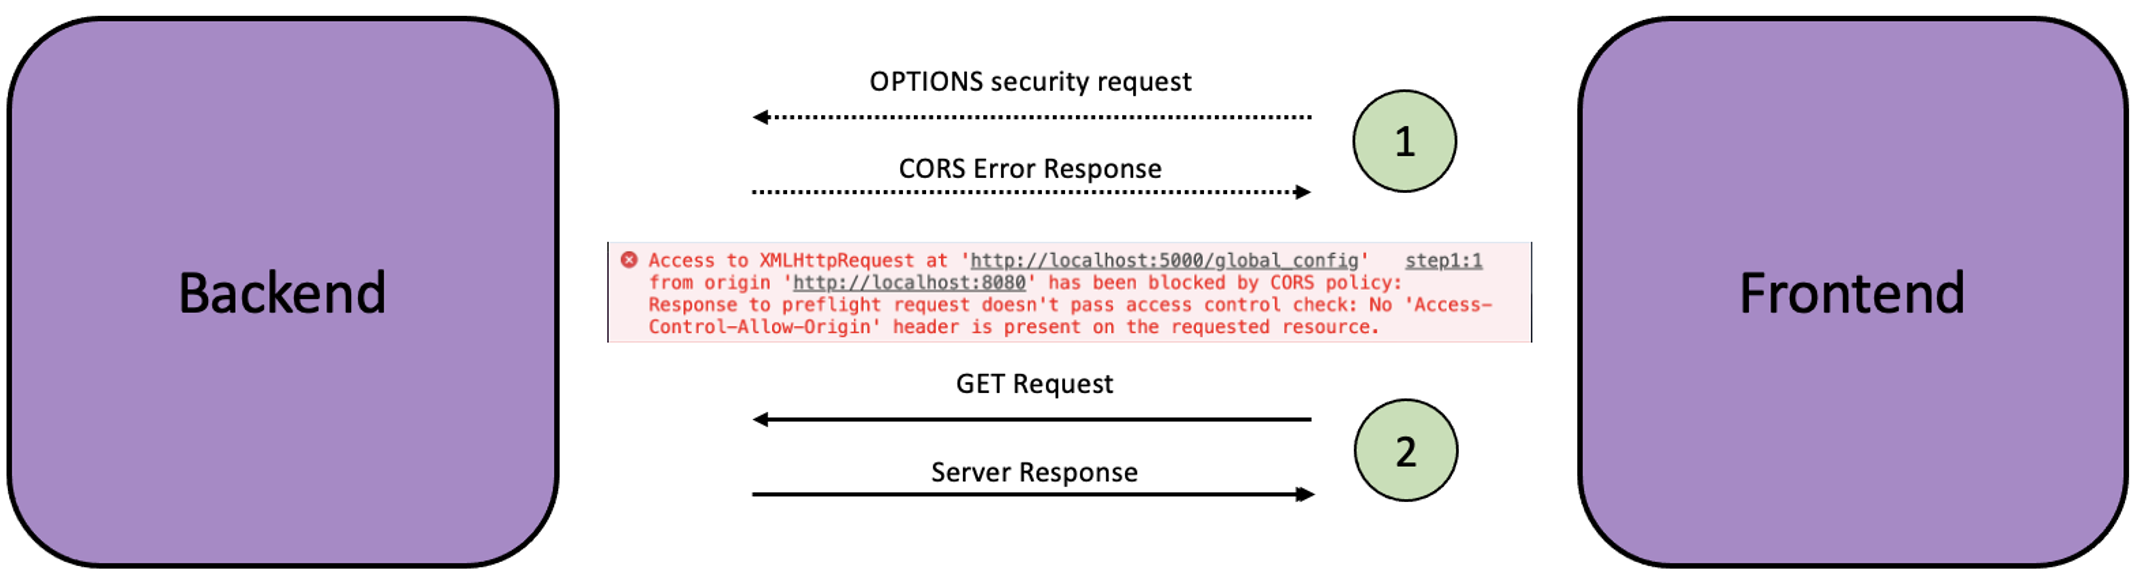
\includegraphics[width=1\textwidth]{images/cors.png}
  \caption{The author faced the technical issue of a CORS error as the backend was not configure to handle OPTION requests.}
  \label{fig:cors}
\end{figure}

To solve the CORS policy error, the author implemented a CORS Handler trait to wrap the back-end server. This class enabled the OPTION requests to the back-end and added the correct response headers to validate the security request. The author had not anticipated the risk of front-end to back-end connection issues as they previously had only interacted with front-end systems in environments with existing solutions to this problem. This error provided the author with the opportunity to learn about inbuilt browser security mechanisms. 

\clearpage

\subsection{Technical Challenge: Generating Test Data}

In order to test the ability of the back-end to generate the Atlas Web from a file system, the author created a series of unit tests which parsed a local file system. As more tests were added to the project, the test results became inconsistent. This was because certain tests invoked PUT requests to update document content which in turn, caused subsequent tests to fail due to incorrect assertions about the document content. To make the tests stateless, the author created a utility class which could create a test file structure. The utility class was invoked before each unit test was ran. The re-creation of the file structure ensured that each test had a consistent environment which had not been manipulated by previous tests. This also enabled the author to omit the test file structure from the repository which reduced the project complexity. Thus, the author learnt the importance of creating clean, stateless unit tests.

\subsection{Methodology Adaptation: Balancing Scrumban Roles}

Overall, the Scrumban methodology complemented the development of Atlas, as it enabled a flexible workflow that could respond to the addition of new requirements. However, the author found it challenging to perform all of the roles required to maintain the Scrumban framework. As the author played the role of both the developer and the product owner, they were required to maintain the responsibilities of both roles. Therefore, in addition to maintaining the Scrumban board, creating the backlog and handling the workflow, they had to also develop, test and deploy the software. During busier periods, the Scrumban board was not updated to reflect current work as the author prioritised development over management practices. In an attempt to maintain the Scrumban methodology, the author tried to update the Scrumban board before they began development. In future projects, the author would try to divide their time better to play the different roles, in an attempt to ensure the framework did not become too overwhelming.

\newpage
\section{Testing and Security}
\subsection{Testing Driven Development}

For the development of Atlas the author used test driven development (TDD). TDD is a software development practice that requires failing unit test to be created before the feature code is implemented (Beck, 2003) (Figure ~\ref{fig:tdd}). Unit tests ensure that individual methods within the code display the intended behaviour. In TDD, software requirements are first converted into test cases before the author codes the solution to the new functionality. This structure forced the developer to think about the intended behavior of the feature and the design of the application. In turn, this resulted in a simpler and more efficient code as the author prioritised the design of the external interfaces (Fowler, 2003). Furthermore, TDD improved the codes reliability and the author's understanding as it encouraged purposeful and consistent test cases (Beck, 2003). This mitigated the risk of a poor code quality (R5). Future developers whom work on the project could use these test cases as a starting point for understanding the intended behaviour of the application.

\begin{figure}[!htb]
  \centering
      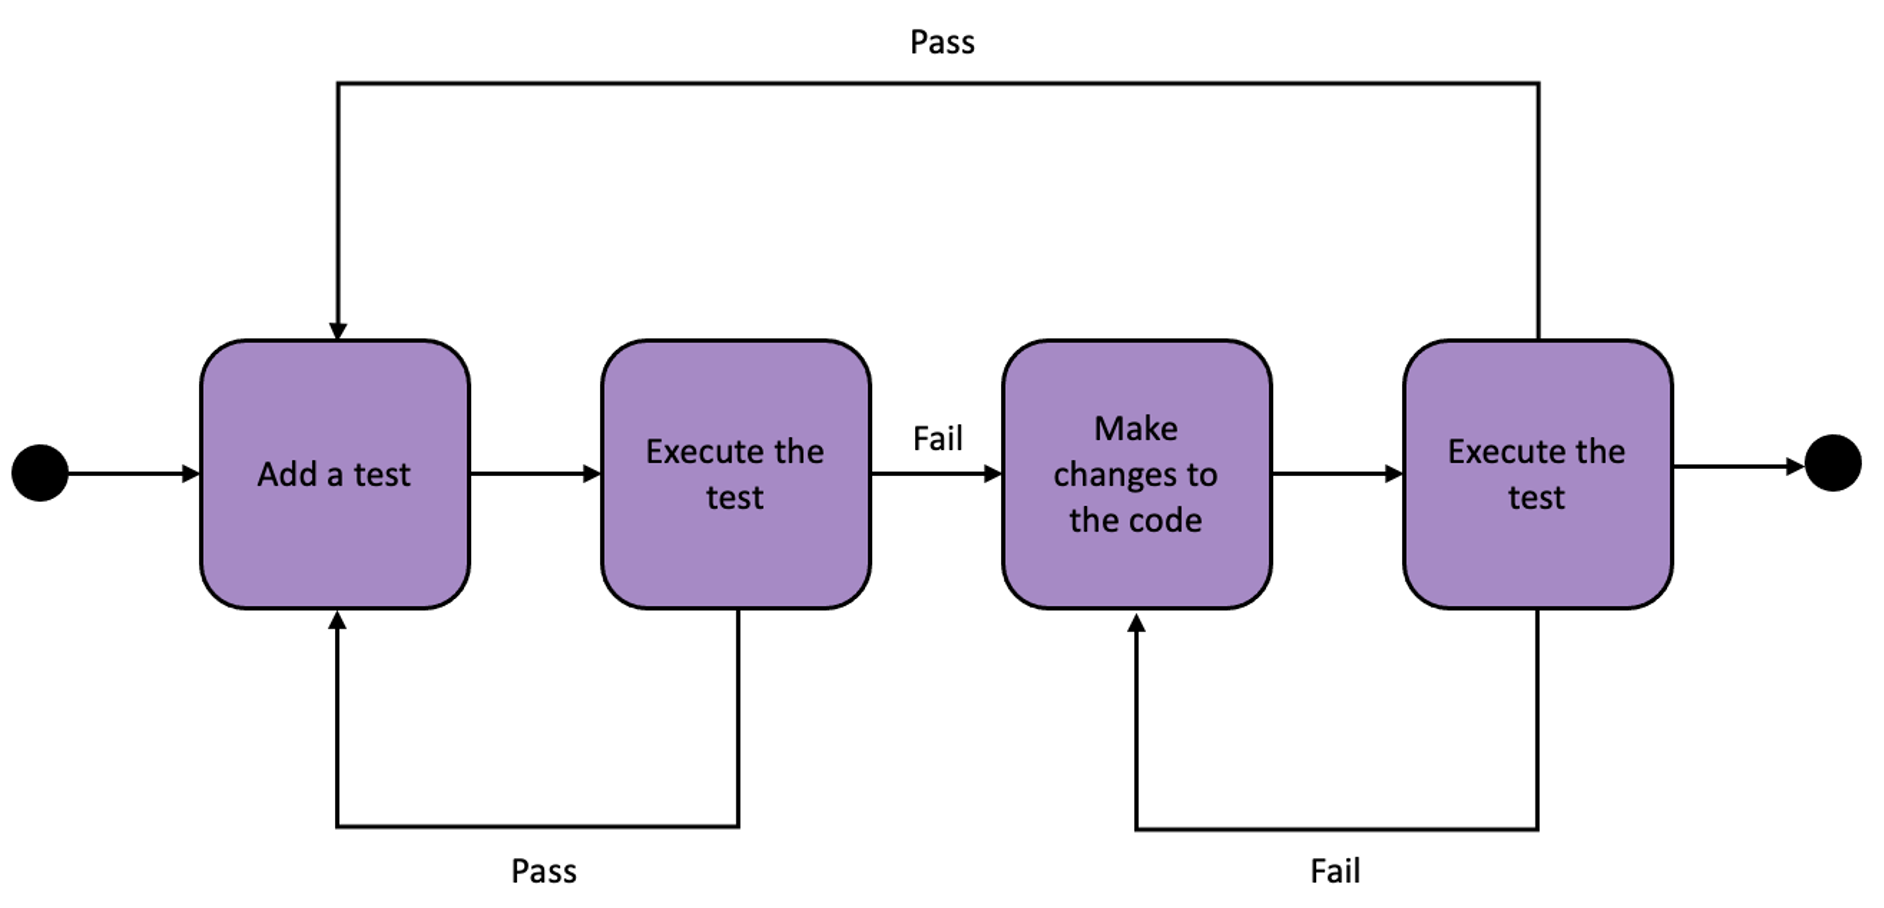
\includegraphics[width=1\textwidth]{images/tdd.png}
  \caption{The Test Driven Development cycle used in the development of Atlas enforced failing tests to be written before the code was implemented.}
  \label{fig:tdd}
\end{figure}

\subsection{Functional Tests}

In addition to unit tests, functional tests were implemented with every new feature. Functional tests validate the system works as intended by exercising the application as a whole (Juristo and Vegas,  2003). Thus functional tests closely mimic the user journey and test the system behaviour at a high level. In order to run the functional tests, the application was containerized with docker. Docker is software that packages an application and its dependencies into a virtual container. Docker can be ran on any operating system, as the virtual container ensures that tests were ran consistently in an isolated environment. Therefore, using docker reduced the chance of technology-specific bugs (Docker, 2021). 

\subsection{Continuous Integration Pipeline}

It is important to regularly test an application during the development period to ensure no new bugs are introduced. The author introduced a continuous integration pipeline that automatically ran all unit and functional tests before a new feature was included in the master branch of the application. The author created the pipeline as a GitHub WorkFlow (GitHub, 2021). The WorkFlow ran all tests before a pull request could be merged into the master branch (Figure ~\ref{fig:githubflow}). The pipeline improved the code quality and reduced the number of manual steps required to release a new feature.

\begin{figure}[!htb]
  \centering
      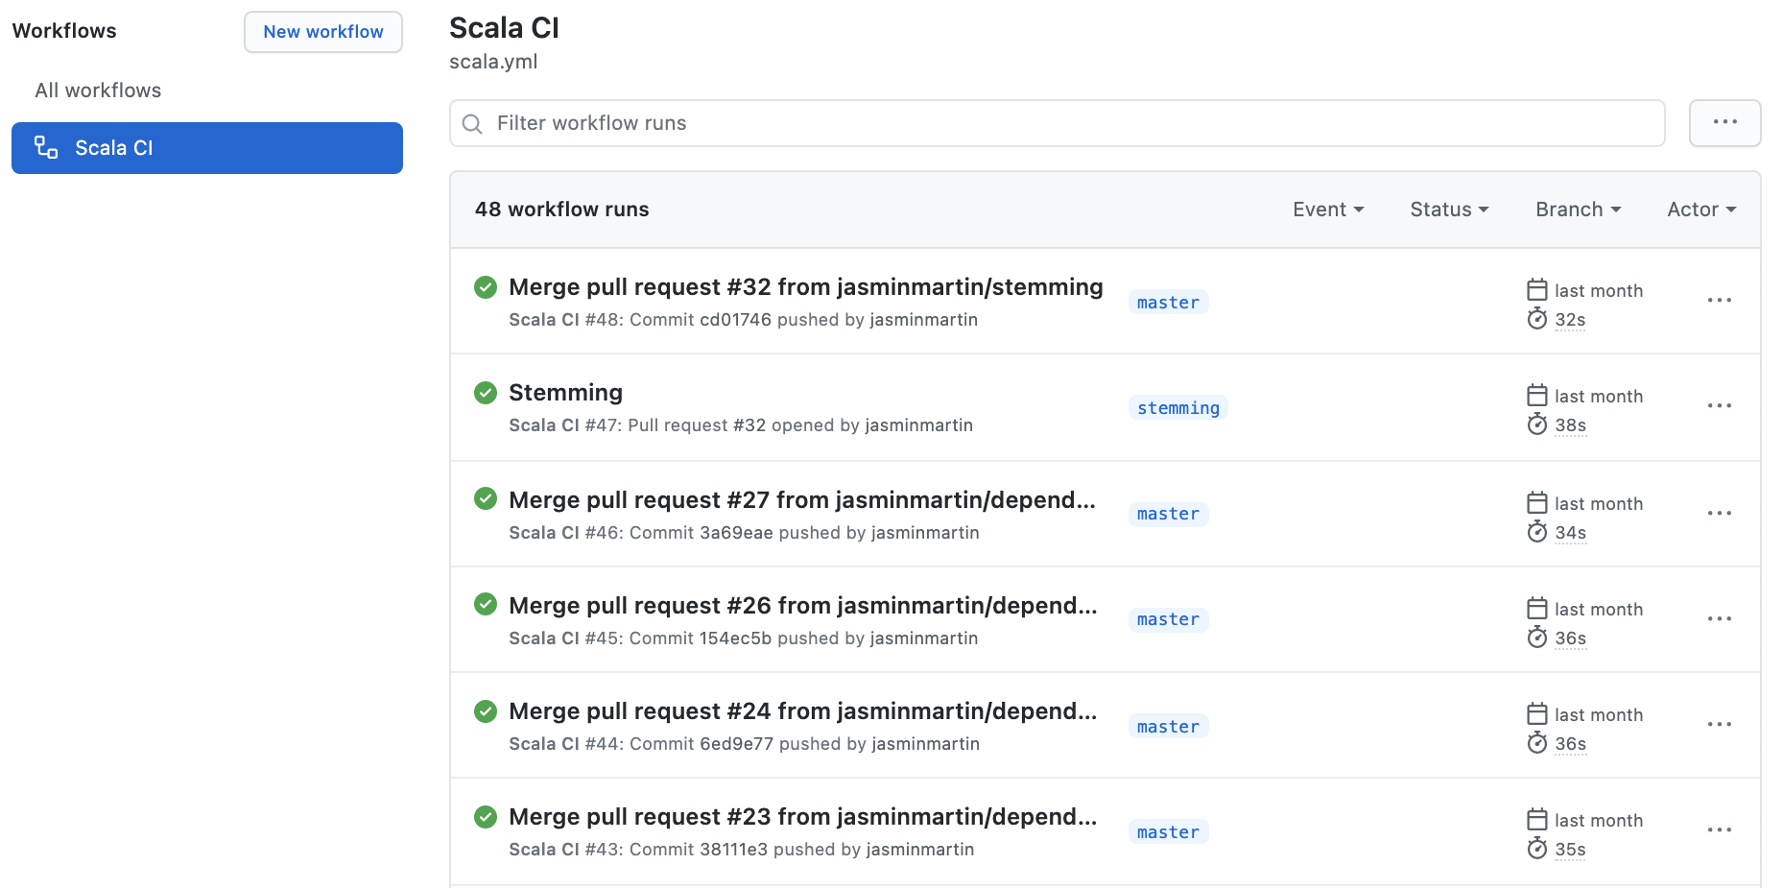
\includegraphics[width=1\textwidth]{images/scala-ci.png}
  \caption{The continuous integration pipeline for Atlas was created as a GitHub Workflow.}
  \label{fig:githubflow}
\end{figure}

\subsection{Non-Functional Testing}
In addition to testing the functionality of the application, the author also tested its performance (NF3). It is important that the application could quickly respond to user commands to provide a smooth user experience. The author created a load test to simulate a user adding and removing 500 documents to and from the Atlas Web within a period of 15 seconds. The author used Gatling to create the load test. Gatling is an open-source load-testing tool that measures the performance of an application (Gatling, 2021). The resultant report revealed that Atlas was able to handle the load without throwing any errors or resulting in high latency above 0.1 seconds.

\subsection{Docker Image Vulnerabilities}

To improve the security of Atlas, the author scanned the application docker image for vulnerabilities. The author used Docker Scan to discover that the application initially contained 38 vulnerabilities; 8 of which were rated highly severe. The vulnerabilities stemmed from Atlas’s dependencies and transitive dependencies. These vulnerabilities could compromise the applications functionality or security (Docker, 2021). 

Docker scan revealed a highly severe vulnerability in the openjdk-11 dependency. This dependency contained a bug that enabled an unauthenticated attacker with network access via multiple protocols to compromise the Java SE (National Vulnerability Database – CVE -2021-2388, 2021). Another moderate rated vulnerability in the GNU C dependency enabled a context-dependent attacker to cause a denial of service by exploiting regular expression bounded repetitions that bypassed the intended limits (National Vulnerability Database – CVE -2010-4051, 2021). The vulnerable packages were upgraded to the safer versions to remove any dependency related security vulnerabilities (Figure ~\ref{fig:dockerscan}).

\begin{figure}[!h]
  \centering
      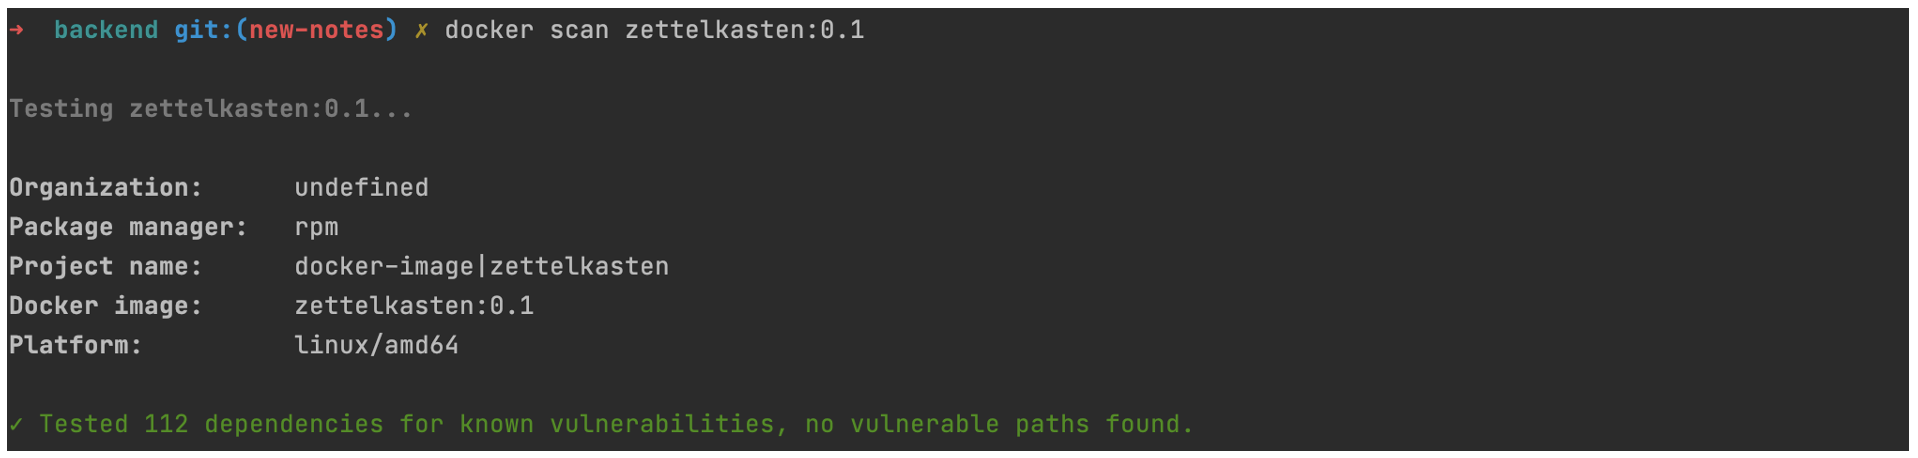
\includegraphics[width=1\textwidth]{images/vulnerabilities.png}
  \caption{A docker scan demonstrating no vulnerabilities found in the dependencies or transitive dependencies of Atlas.}
  \label{fig:dockerscan}
\end{figure}

In addition to upgrading the vulnerable dependencies, the author also changed the applications base image to be distroless. Distroless images only contain the application code and the run-time dependencies. They lack the package manager, shells and operating system typical in a Linux distribution. Using a distroless image not only reduces the number of potential packages containing vulnerabilities, but also makes the application less prone to surface attack as there is no shell to access the container (Moore, 2017). By removing the shell, a potential attacker cannot read any secrets on the container or secure information persisted such as user files (Figure ~\ref{fig:distroless}). This also prevents the installation of any untoward packages. The distroless image also had the additional benefit of being 35\% smaller.

\begin{figure}[!htb]
  \centering
      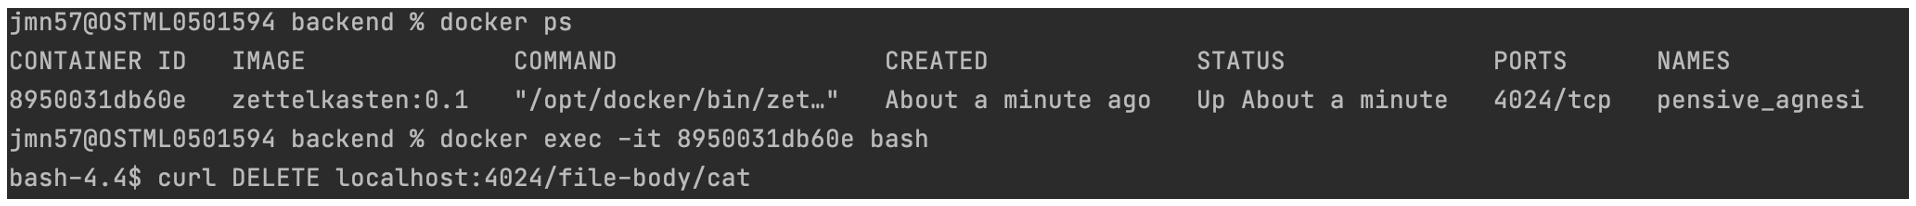
\includegraphics[width=1\textwidth]{images/distroless.png}
  \caption{An attacker could easily delete user documents in Atlas if it utilised a non-distroless base image.}
  \label{fig:distroless}
\end{figure}

\subsection{Dependabot Library Upgrades}

To prevent further transitive dependency vulnerabilities, Dependabot alerts were enabled on the Atlas GitHub repository. The Dependapot actively scanned libraries for any vulnerabilities on a daily basis (Figure ~\ref{fig:dependabot}). The author could upgrade libraries from the GitHub interface, which would in turn run the continuous integration pipeline to ensure the upgrade did not inhibit the applications functionality. 

\begin{figure}[!ht]
  \centering
      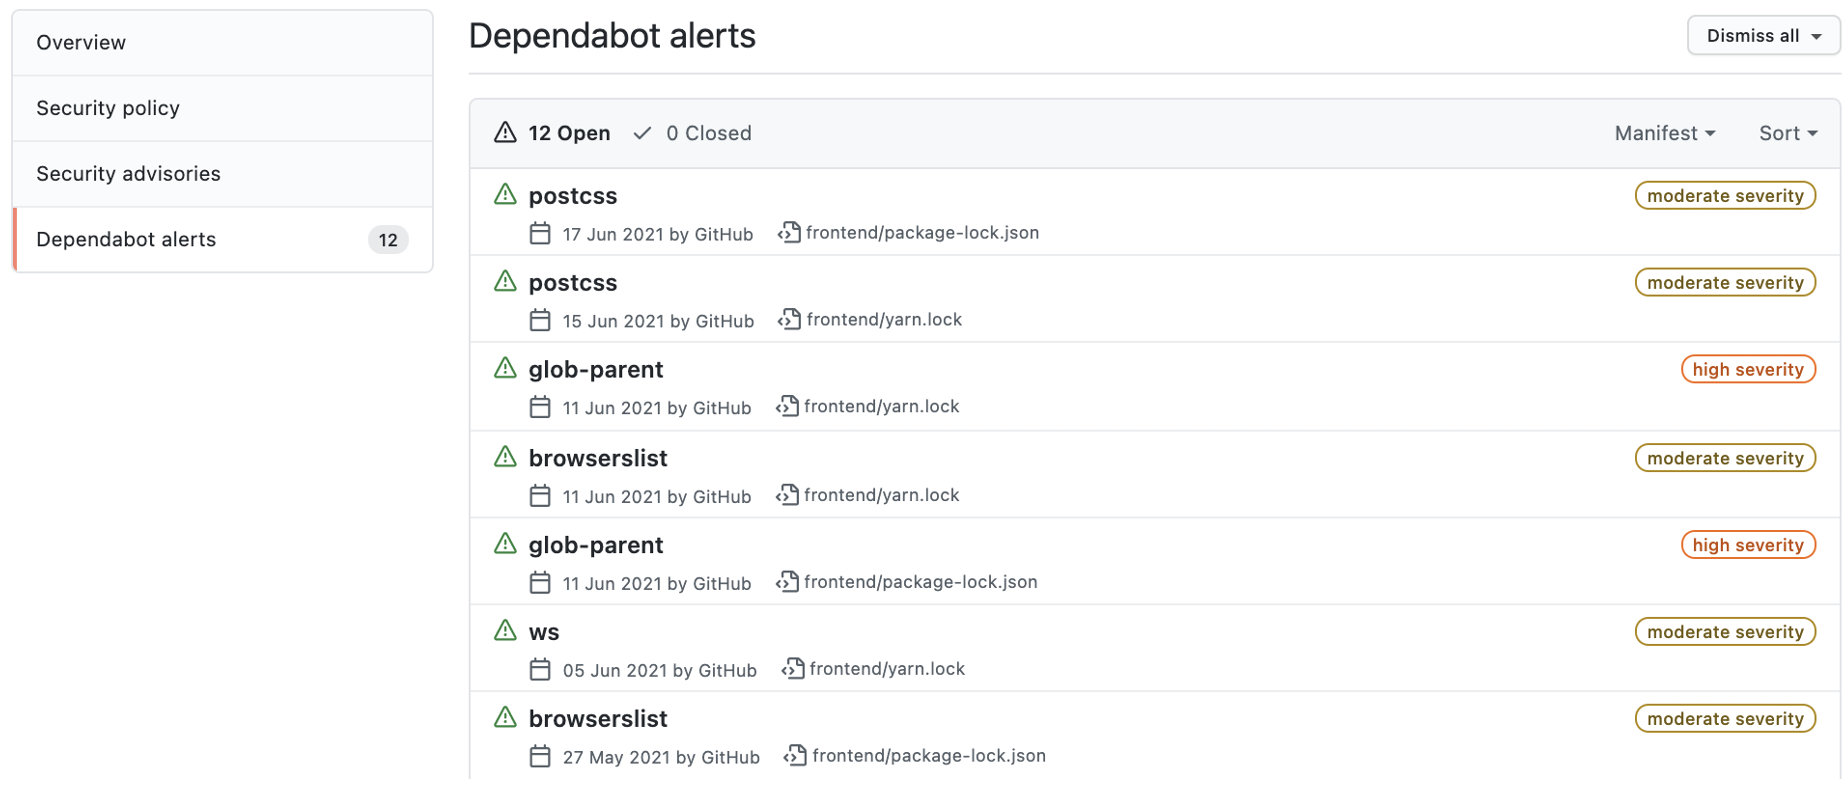
\includegraphics[width=1\textwidth]{images/dependabot.png}
  \caption{Dependabot alerts signalling library upgrades are required in the Atlas repository to prevent vulnerabilities.}
  \label{fig:dependabot}
\end{figure}

 
\clearpage
\section{Implementation}

\subsection{Local Artefact}
Atlas is available as a local artefact on GitHub at \url{https://github.com/jasminmartin/atlas}. The application code is open source; it is available to view, run or extend by members of the public. The GitHub repository is complete with documentation in the readme.md which advises users on how to run the application. The Latex project report and images are contained within the repository along with instructions on how to generate this accompanying PDF.

\subsection{Deployment Strategy}
The author had planned to release Atlas onto the Google Cloud Platform (GCP) - their organisation's chosen cloud computing provider. The cloud is a system of servers located in data centres all over the world (Pratim, 2018). The back-end and front-end of Atlas would be hosted in separate Kubernetes pods in which scaled individually to meet client load. Client requests would be directed with ingress that would enable access to the cluster.

\begin{figure}[!b]
  \centering
      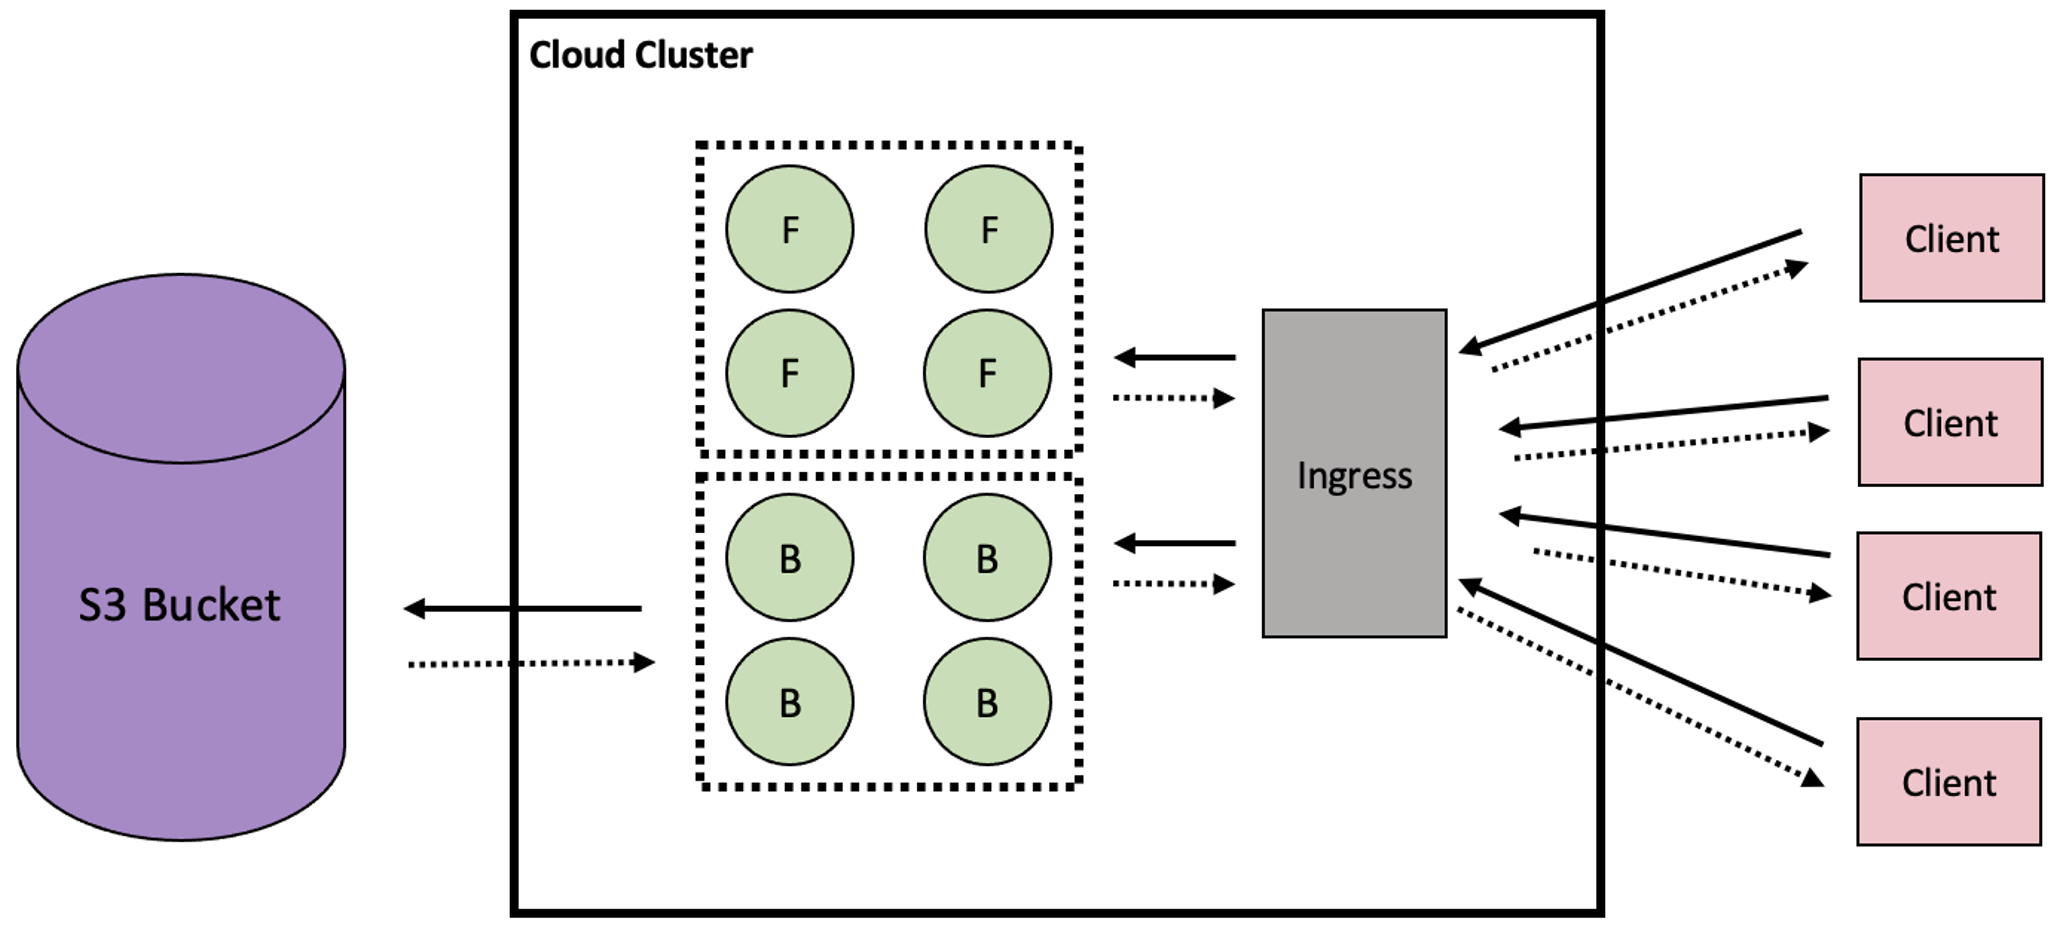
\includegraphics[width=1\textwidth]{images/deployment.png}
  \caption{Cloud-based architecture of Atlas. The green ‘F’ and ‘B’ circles represent the front-end and back-end pods.}
  \label{fig:deploy}
\end{figure}

Before the application was deployed to GCP, the author would modify the application architecture so that documents were stored in a Amazon S3 bucket (Figure ~\ref{fig:deploy}). This would ensure documents could be accessed by multiple members of the organisation with consistent content.

To deploy new versions of Atlas to the cloud, the author would develop a continuous integration continuous deployment (CICD) pipeline. CICD pipelines automate the software delivery process by automatically building code, running tests and deploying to different environments (Freeman, 2018). The former two processes were utilised in the development of Atlas with the aid of a GitHub WorkFlow. In order to include continuous deployment into the pipeline, a more appropriate CICD pipeline solution would be used such as Jenkins. The author's organisation has configured Jenkins to deploy applications into a number of gated GCP environments. Each environment tests a different element of the service. For instance, a non-functional environment may test the application can handle simulated high loads, whilst an integration environment could enable developers to manually test features before they are released to production (Jenkins, 2016) (Figure ~\ref{fig:jenkins}).

\begin{figure}[!htb]
  \centering
      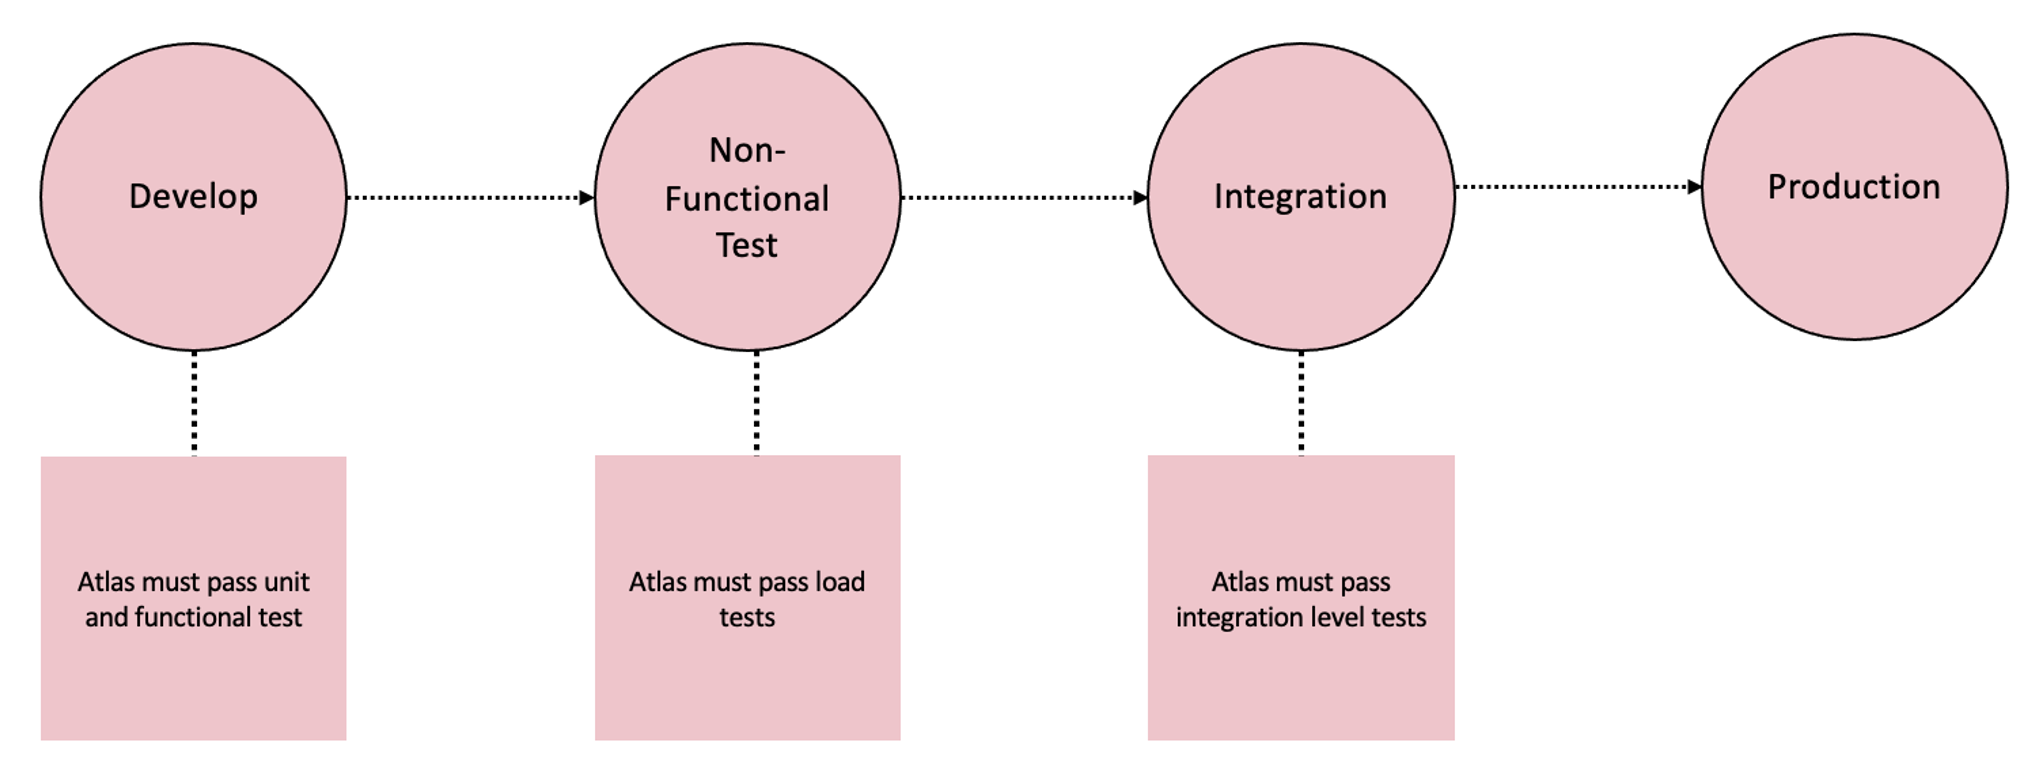
\includegraphics[width=1\textwidth]{images/jenkins.png}
  \caption{Jenkins pipeline setup could release the Atlas application into different testing environments before it is released to production.}
    \label{fig:jenkins}
\end{figure}

\subsection{Metrics and Monitoring}

In order to provide a good level of service, it is important to maintain the performance and availability of a software application. Before Atlas is released into a production environment, the application must be able to generate and surface metrics. These metrics would be monitored to measure and alert the author to any problems with the user experience. Using the Kamon metrics instrumentation, the author could surface metrics that measured the traffic load, response time and response status codes (Kamon, 2021). These metrics could be visualised using a monitoring dashboard such as Grafana (Figure ~\ref{fig:grafana}) (Grafana, 2021). Deviations of metrics above alerting thresholds could indicate problems with the infrastructure or application functionality. For example, a high percentage of requests resulting in 404 status code responses could indicate a bug within the application. 

\begin{figure}[!htb]
  \centering
      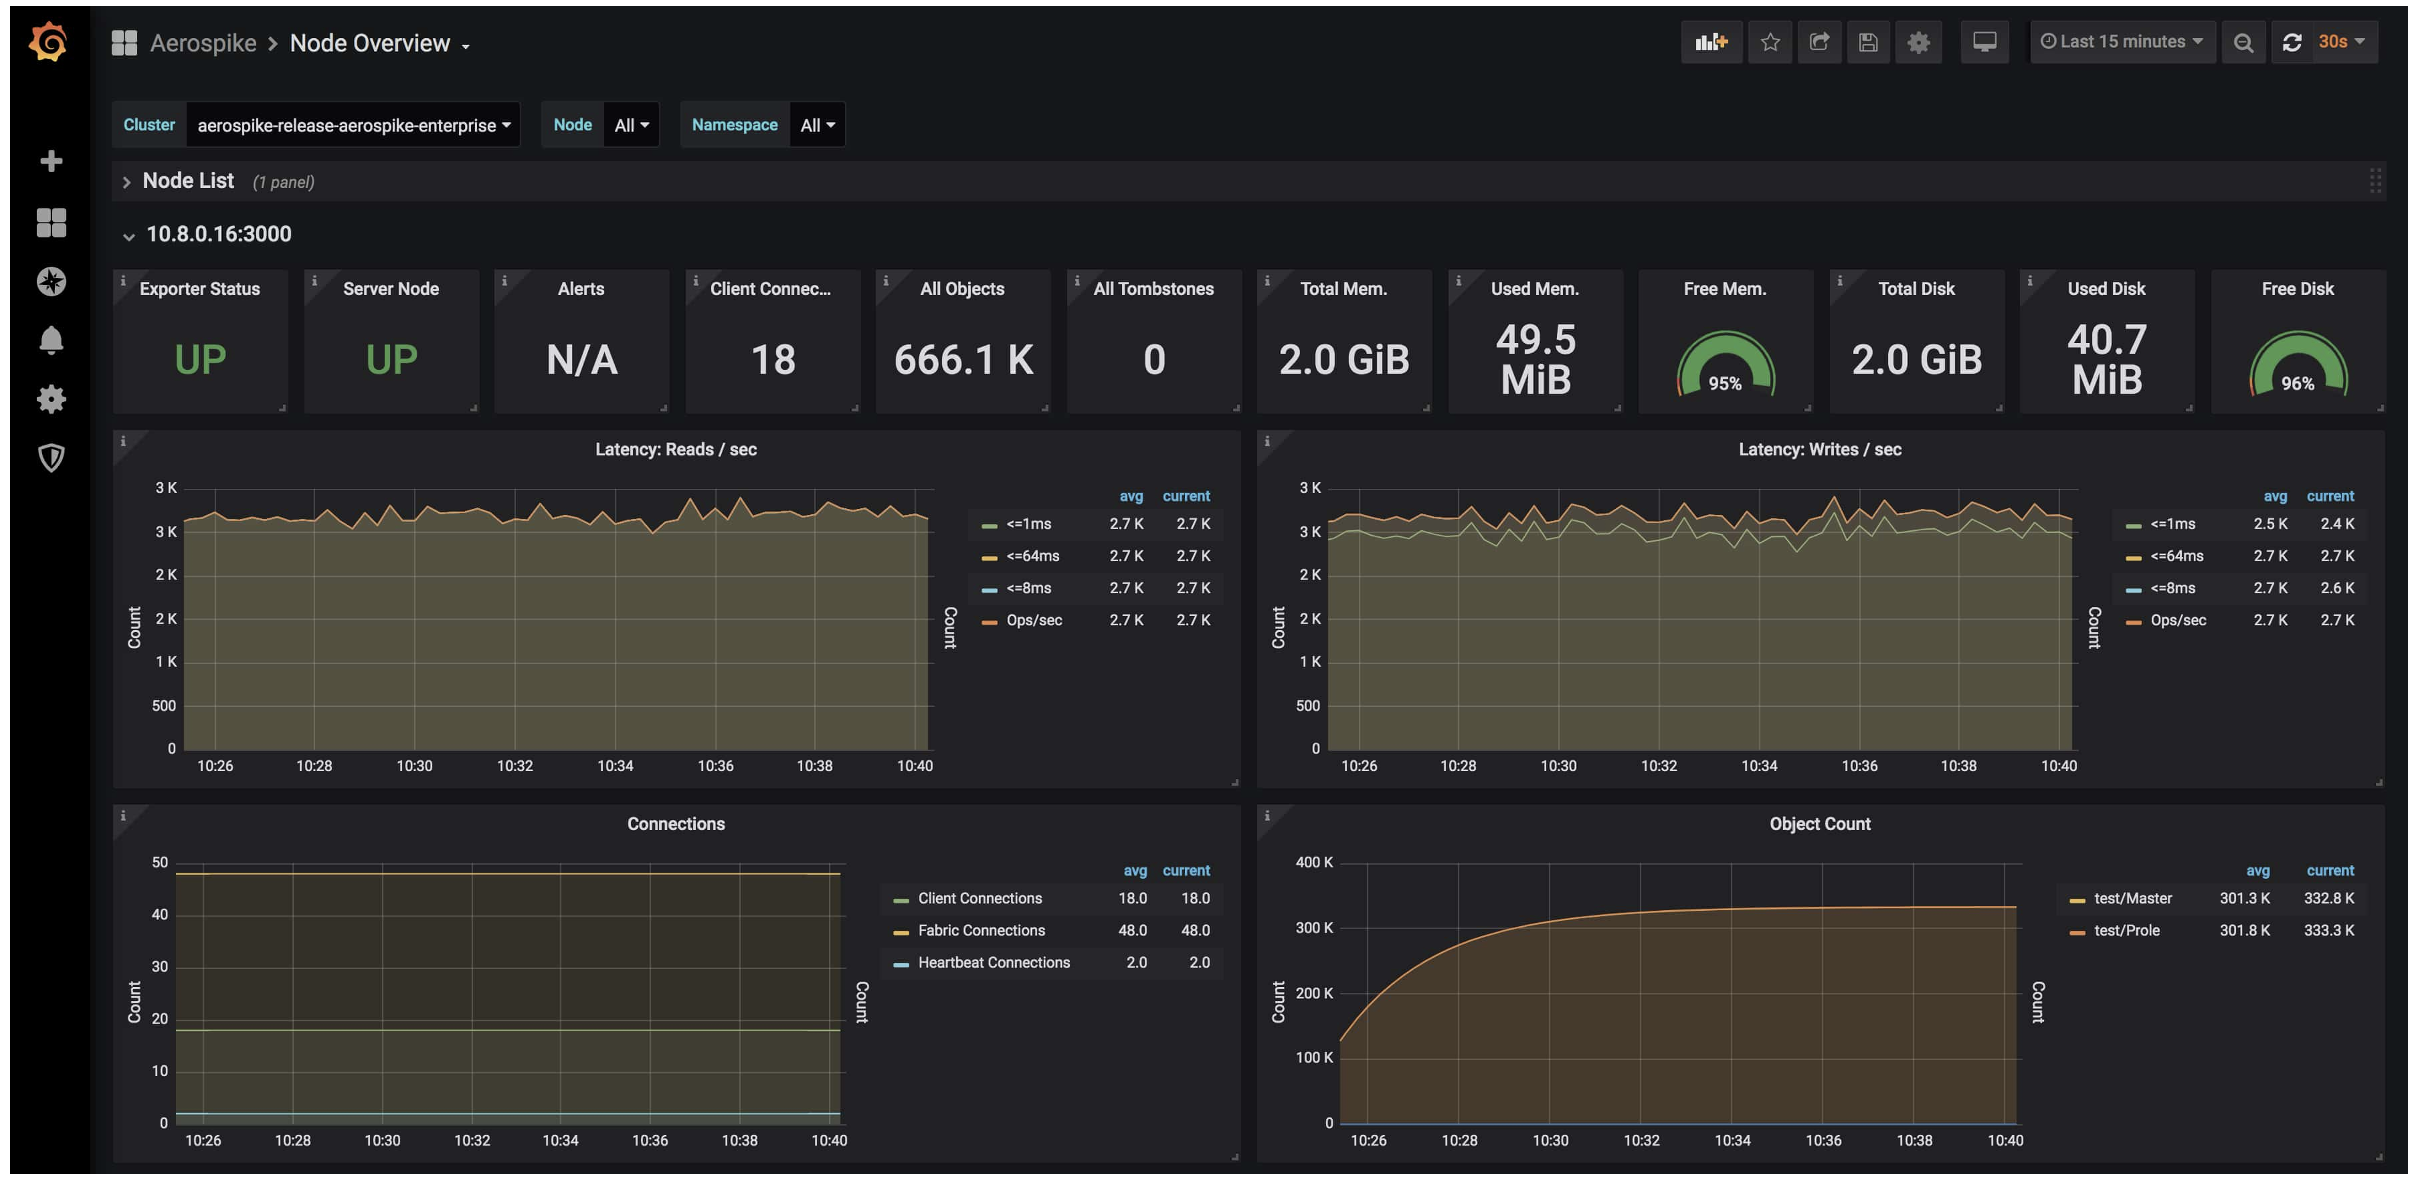
\includegraphics[width=1\textwidth]{images/grafana.png}
  \caption{An example of a Grafana monitoring dashboard that alerts the developer of problems in a production environment (Pujari, 2019).}
  \label{fig:grafana}
\end{figure}

In addition to monitoring the API responses, it is also important to measure metrics related to computational resources usage. By understanding the CPU and memory usage of an application, the developer can predict the financial cost of running the application. Incorrect resource allocation could risk financial wastage or result in poor application performance (Pratim, 2018). Atlas would be deployed onto GCP which provides an on-demand variability of computing resources. Although this means that pods can auto-scale to increase resource availability to meet load, it is still important to monitor resource usage as unexpectedly high resource usage may indicate issues with memory management in the application (Pujari, 2019).

\subsection{Further Functional Requirements}

As Atlas was developed using an agile management style, it would be possible to release the application in its current incrementation. However, future functional requirements could be added to improve the user experience (Table 10). The author did not fully develop the automatic keyword suggestion feature (F8). As this ability would make the application unique from competing knowledge management tools, prioritising this feature could significantly increase product uptake and department interest. To implement this feature, the author would build upon their knowledge of the Play framework which would enable the application to efficiently store and recommend common keywords.

To use the aforementioned deployment strategy (Figure ~\ref{fig:deploy}), Atlas would have to be modified so that it could maintain consistent content of shared documents (F11). This functionality would enable users in large organisations to easily update shared documents. As Atlas is currently configured to work with local file systems, to achieve this the application would have to be integrated with an Amazon S3 bucket which would hold the state of the documents.

Although synthetic monitoring systems such as Dynatrace offer a thorough solution to monitoring user journeys, they require a subscription and maintenance cost (Dynatrace, 2019). Whilst the customer base of Atlas is low, the author could implement a cheaper solution; collecting feedback via embedded in application surveys (F12). Such feedback could surface problems with the application usability, or uncover application bugs. Customer feedback widgets are one of the most common devices for gathering application feedback. Adding a short survey in the context of the application offers a convenient way for customer to submit feedback. Such methods are proven to have higher response rates than email surveys (Spiess et al., 2012). 

\begin{table}[]
\centering
\small
\caption{Potential future functional requirements to be implemented into Atlas.}
\label{tab:my-table}
\resizebox{\textwidth}{!}{%
\begin{tabular}{|l|p{16cm}|}\hline
\textbf{No.} & \textbf{Functional Requirement} \\ \hline
\textbf{F8} & To automatically suggest new connections \\ \hline
\rowcolor[HTML]{FFCE93} 
\textbf{F11} & To maintain consistent shared documents \\ \hline
\rowcolor[HTML]{FFCE93} 
\textbf{F12} & To collect feedback via an embedded survey \\ \hline
\end{tabular}%
}
\end{table}

\newpage
\section{Conclusion}

The development  of Atlas provided the author with a mechanism for improving their project management and technical skills. Creating a greenfield application gave the author the opportunity to develop a product through the whole application life cycle; from soliciting requirements, to designing and implementing the user interface and experience. The author was guided through the development process with their chosen Scrumban Agile methodology. This project management style provided a framework for the author to iterate upon the application whilst gathering and incorporating user feedback. Throughout the process, the author was able to interact and build working relationships with different members of the department whilst developing a tool which could improve productivity in the organisation. 

In total, the author achieved three of the four initial objectives, resulting in a functional iteration of Atlas. Although the application was not deployed into a production environment, the resulting local artefact forms a strong basis which with further work, could be used to improve the comprehension of the organisation's documentation. User feedback on the current iteration suggests Atlas provided a clear user interface that offered a more intuitive experience than the hierarchical file system.

The author considers the project to be a success as it improved both their organisational and technical skills. In particular, they improved their front-end development abilities, as they became more confident using the React framework. The author also learnt more about natural language processing techniques, and formed an interest in big data manipulation which they would like to pursue further in the future.

\newpage
\section{Further Work}

For Atlas to be used in an organisational setting, it must be deployed into a production environment. The aforementioned deployment strategy could be executed within an 8 week development period (Figure ~\ref{fig:further-work}). First, a small functional change to the document storage would enable Atlas to be deployed onto the cloud (F11). The author would also implement metrics and monitoring to guarantee the application is running smoothly in production. As the author's organisation already uses Jenkins pipeline infrastructure and GCP environments are already configured, the author estimates it would only take a further 4 weeks of development to deploy Atlas into production. Once deployment had been completed, the author would prioritise the automatic tag recommendation (F8) as the next developed feature as they have already researched big data processing frameworks.

\begin{figure}[!htb]
  \centering
      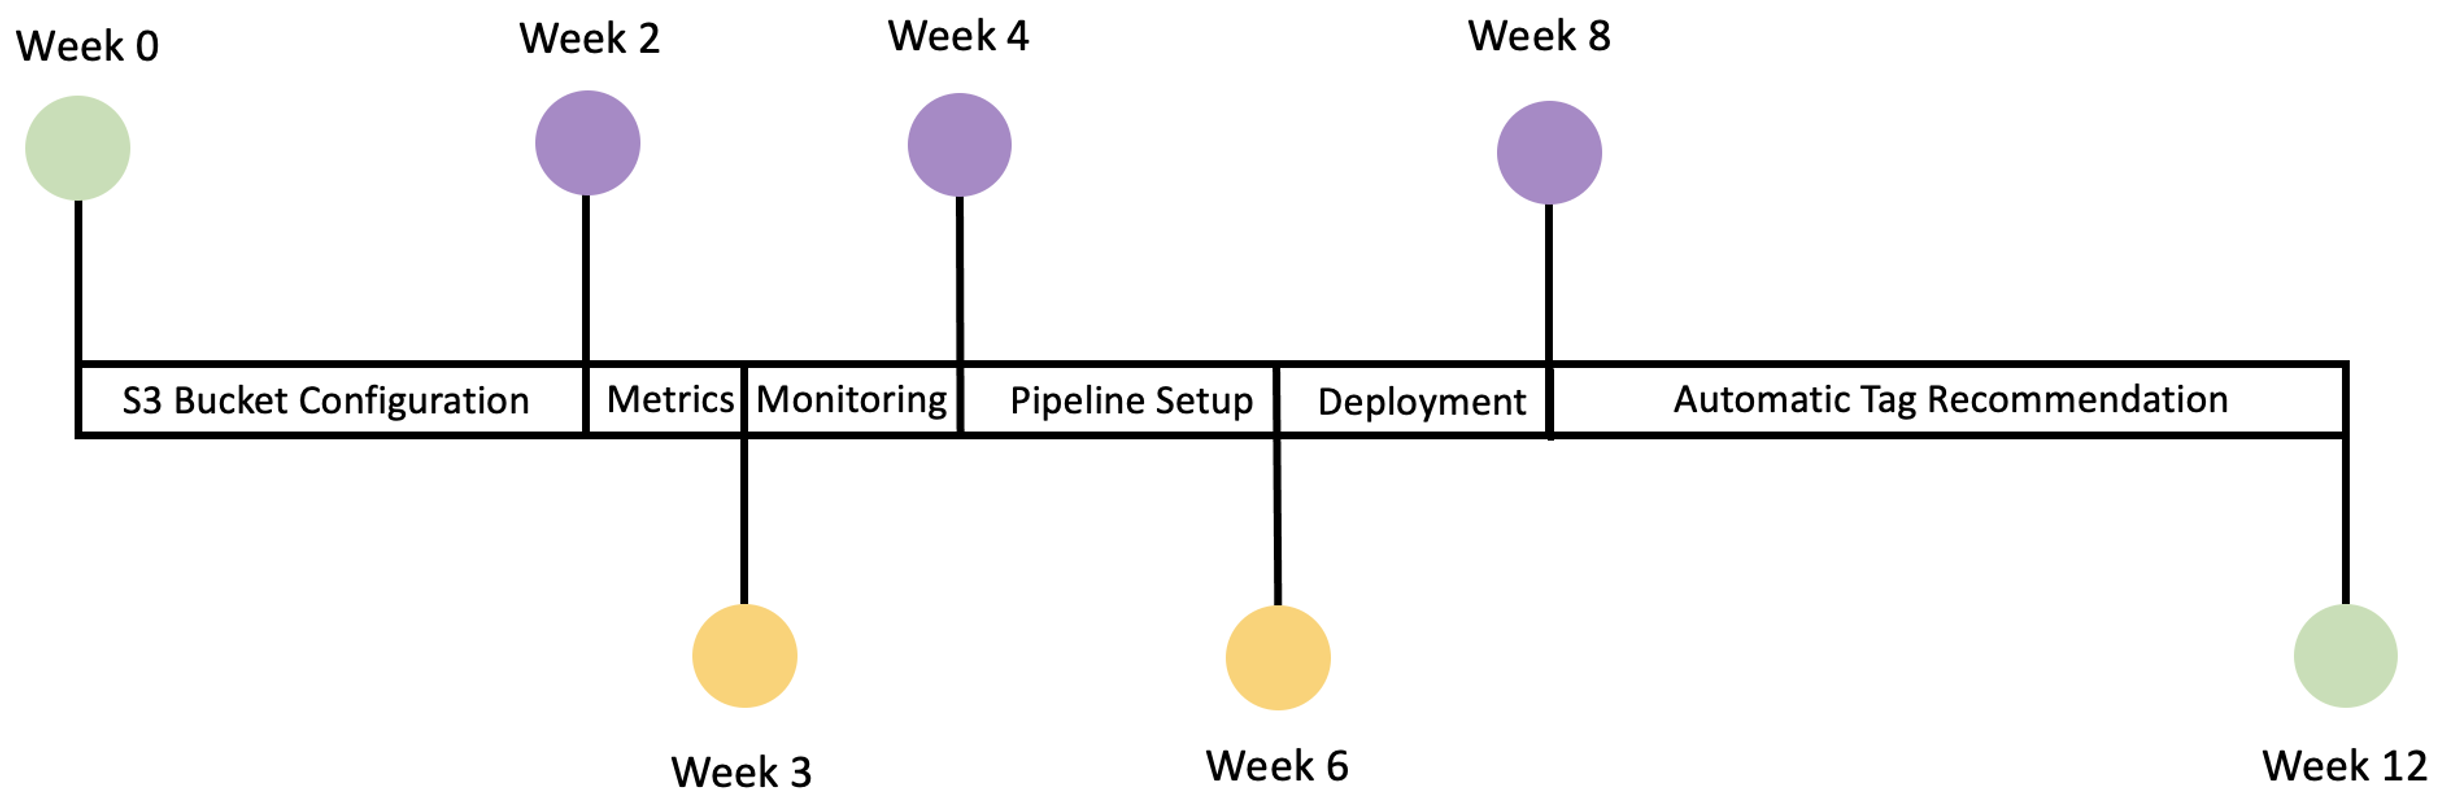
\includegraphics[width=1\textwidth]{images/future-timeline.png}
  \caption{The author would dedicate the next 8 weeks of development to ensuring Atlas was ready to be deployed into production. A further estimated 4 weeks could then be used to develop the automatic tag recommendation feature.}
  \label{fig:further-work}
\end{figure}

In addition to developing the application functionality and infrastructure further, the author would also dedicate effort to introducing more developers in the organisation to Atlas. As the product will remain with the organisation, it is important to future-proof the application by ensuring other developer have context of the code and understand the related documentation. The author could engage more developers into the project by demoing the deployed product in the department showcase and encouraging audience members to take part in the next stages of development.

\newpage
\section{Reflective Statement}

Over the course of the synoptic project, the author built upon their behavioural and technical skills. Both the project management and technical development of Atlas gave the author the opportunity to exercise and evaluate the abilities defined in the apprenticeship standard. Drawing upon examples from the development of Atlas, here the author reflects on how three specialist technical competencies and three core behavioural skills were improved over duration of the course (Table 11). Furthermore, the author applies the Gibbs behavioural model to their personal experiences in an attempt to understand how they can further their abilities (Gibbs, 1997). Evidence towards other apprenticeship standard skills can be found in \hyperref[sec:appendix-3]{Appendix 3}.

\begin{table}[!h]
\small
\caption{The Specialist Technical Skills and Corse Behavioural Skills that were improved by the author over the duration of the synoptic project.}
\label{tab:my-table}
\resizebox{\textwidth}{!}{%
\begin{tabular}{|p{1cm}|p{14cm}|}
\hline
\textbf{Id} & \textbf{Skill Description} \\ \hline
STS-1 & Create effective and secure software solutions using contemporary software development languages to deliver the full range of functional and non-functional requirements using relevant development methodologies. \\ \hline
STS-2 & Test code to ensure that the functional and non-functional requirements have been met. \\ \hline
STS-3 & Deliver software solutions using industry-standard build processes, and tools for configuration management, version control, and software build, release and deployment into enterprise environments. \\ \hline
CBS-1 & Makes concise, engaging and well-structured verbal presentations, arguments and explanations. \\ \hline
CBS-2 & Applies analytical and critical thinking skills to Technology Solutions development and to systematically analyse and apply structured problem-solving techniques to complex systems and situations. \\ \hline
CBS-3 & Able to conduct effective research, using literature and other media, into IT and business related topics. \\ \hline
\end{tabular}%
}
\end{table}


\subsection{STS-1: Developing Functional and Non-Functional Requirements}

The author selected and applied the Scrumban agile framework to ensure the functional and non-functional requirements were iteratively developed using Scala in the synoptic project. They felt Scrumban was appropriate because it complemented both the time period and the size of the project. However, the author failed to consider the fact that they were the sole person in the framework, and as a result, spent a lot of time playing the roles of the scrum master, product manager and developer. Consequently, they felt overwhelmed at times with the amount of organisation and administration needed to maintain all three roles. 

This experience taught the author that process heavy frameworks may not be appropriate for individual developers, and may require adaptations. Despite this, they do not regret applying an organisational framework, as it gave them a taste of how the product management style could operate in the workplace. The author felt that if they were to solely develop a product again, they would take inspiration from a product management style, rather than implement the whole framework. For instance, if they chose Scrumban again, they could utilise the Kanban board and progressive backlog, but not worry about estimating tickets. Moreover, if a project management style was not fitting the project, the author would not be afraid to step outside of the framework before it became overwhelming.

\subsection{STS-2: Testing Functional and Non-Functional Requirements}

As part of their synoptic project, the author engaged in test-driven development (TDD) to test the functional requirements via unit tests. The author felt that TDD enabled them to build confidence in their code as it ensured each method was tested. Furthermore, they were surprised to find that the style also encouraged them to plan and organise features better. The author enjoyed TDD as it acted as a framework for reviewing and improving their own code. The author has since brought this practice into their workplace and has found it has helped to align coding styles when pairing.

To ensure non-functional requirements were met, the author introduced load-style gatling tests. Although the load test ensured the application could cope with spikes in traffic, on reflection, the author would spend less time implementing such a large scale framework in the future. As the application was only used simultaneously by a few people, the author did not believe such thorough testing was needed. Instead, if the author was to test the non-functional requirements again, they would take the opportunity to measure the security and user experience of the application. The author realised that they had not collecting enough metrics on these areas and would be interested in researching industry practices to collecting these metrics. Moreover, as the author is predominantly a back-end developer, they would be interested to see how front-end elements such as user journey experiences could be improved.

\subsection{STS-3: Delivering Software Solutions}

The author particularly enjoyed delivering software solutions by engaging in all areas of the product life-cycle; from build to deployment. As the author had predominately engaged in the build side of the life-cycle and already knew how to use version control and configuration management in the workplace, they felt the apprenticeship helped them understand the whole life-cycle process and appreciate how the solution is delivered to customers. In turn, the author felt more engaged with the users of their product as they understood how they interacted with the application from a technical perspective. However, at times they did feel constrained by the organisations choice of technology. For instance, the organisation favoured the Jenkins pipeline instead of CircleCI – which is a more common industry solution (Frankinson, 2020). Instead of becoming frustrated, the author learnt to accept the limitations of the organisation's choices and instead, tried to understand why certain technologies had been selected from a business approach. This helped them understand the build processes within the business.

\subsection{CBS-1: Verbal Communication}

In order to gather feedback to incorporate into the design of Atlas, the author showcased the application in a series of presentations. In order to ensure the presentations encouraged detailed feedback, the author researched how to tailor the content to the demographic of the audience. For instance, in  presentations with a non-technical audience, the author ensured they used non-technical language and focused on high level concepts rather than technical implementations. The author also improved general presentations skills by reducing the amount of text in the presentation to make it more concise and by incorporating more diagrams to maintain the interest of the audience. 

The author was happy with their progress in improving their verbal communication skills, as they felt they were able to better to showcase their product which in turn produced higher quality feedback. The author had not previously conducted focus groups or interviews, so the synoptic project gave them the opportunity to structure explanations in a less rehearsed format. A key difference the author found between these formats was that the author's role was more focused on persuading and engaging the audience through the process, rather than just explaining. The author was able to use their leadership skills to guide the discussions of others, rather than detail arguments upfront. Moreover, the showcases improved the author's confidence and the positive feedback from the audience motivated them. If the author was to conduct product research again, they would be more likely to showcase the product to larger audiences.


\subsection{CBS-2: Applying Critical Problem Solving to Technology Solutions}

The author was tasked with architecting the project design. As this was a greenfield project, they were able to choose the technology and infrastructure that would support the application in a production environment. The author researched into different languages and frameworks that could support the application. They ensured the technologies were able to efficiently and quickly generate the graph as well as display it in an appropriate fashion. The author chose React Typescript as a front-end framework after comparing it to other popular frameworks. The author enjoyed using React, as they found it intuitive to use and were supported by a large amount of online documentation. Moreover, React allowed the author to create reusable components which reduced the amount of code needed to render the graphs. The author learnt to not become overwhelmed with the amount of technical solutions available, and instead, research and trial the technology to see if it was appropriate.

The author was also able to improve their back-end abilities by researching natural language processes which would enable them to efficiently generate the Atlas graph. The author used an tokenizing algorithm that simplified the ability to select common keywords in the application. The author took an interest in natural language processing and also used the Porter stemmer algorithm to standardise the document file names. The author learnt that by adapting well known algorithms, they were able to build upon existing computer science solutions to complex problems. 

\subsection{CBS-3: Conducting Research}

In the early stages of development of the synoptic project, the author researched a series of literature to form an understanding of how to efficiently create their application. The author conducted a literature review on related content such as project management techniques and technical processes. From their previous experience, the author knew to use tools such as Google Scholar to find relevant papers. However, the author found it difficult to find relevant technical content, and instead, found looking at online articles as a starting point to give a general overview on a technical matter to be more efficient. The author was initially surprised this made the research more effective, but found it significantly decreased the level of understanding required to approach a technical subject.

In order to conduct research into the business needs, the author analysed the current procurement processes. The author was required to design and execute a primary research plan within their organisation. This exercised the author's planning and investigation skills, as they were tasked with finding the appropriate teams to communicate with and organise meetings. On reflection, the author would begin the research process earlier into the project timeline as they found it time consuming to schedule talks with different organisation members. Overall, the experience taught them to use several different information sources to build a more rounded opinion.

\newpage
\section{Glossary}
{\parindent0pt
\textbf{Agile}: A software development methodology focused on iterative cycles of development. Requirements and results are continuously evaluated to quickly respond to change.

\textbf{API}: Application Programming Interface is a software intermediary that enables two applications to communicate with each other.

\textbf{Atlas Web}: The main user interface of the Atlas application that displays the file system as a graph.

\textbf{Auto-Scaling}: a cloud computing process that dynamically adjusts the amount of computational resources with traffic load.

\textbf{CICD}: Continuous integration continuous deployment is the combined practice of building and releasing code into a production environment.

\textbf{Cloud Computing}: An on-demand availability of computer system resources and data storage, that does not require direct active management. 

\textbf{Cluster}: A shared group of networking resources for kubernetes pods.

\textbf{CORS}: Cross-Origin Resource Sharing is an HTTP-header based mechanism that secures browsers by limiting the domains and ports from which resources can be received.

\textbf{CPU}: The Central Processing Unit is the electronic circuitry that runs computer systems.

\textbf{CRUD Request}: Create, read, update and delete requests are the four functions necessary to implement mutable persistent data.

\textbf{cURL Request}: client URL is a command line tool that can be used to make requests to a website.

\textbf{Docker}: a containerized platform that combines the application source code, libraries and operating system into a specific environment.

\textbf{Extreme Programming}: A software development methodology focused upon improving software quality and the speed of response to changing customer requirements.

\textbf{GCP}: Google Cloud Platform is a provider of cloud computing resources for developing, deploying, and operating software applications.

\textbf{Github}: A website that hosts software and acts as a version control system.

\textbf{Github Workflow}: a configurable automated process that is ran on GitHub before code is merged into the master branch.

\textbf{Ingress}: an API object that provides external access to a Kubernetes cluster.

\textbf{Jenkins}: An automation pipeline which enables software to be built, tested, and deployed into different environments.

\textbf{Kanban}: An agile workflow management method for defining, managing and improving software development.

\textbf{Kubernetes}: A container-orchestration system for automatically deploying, scaling, and managing applications in pods.

\textbf{Lemmatisation}: The process of grouping together the inflected form of a word. The lemma of running, runner and runs is run.

\textbf{Pod}: Point of delivery, is a module of application components, storage and network resources that work together to deliver a service.

\textbf{Porter Algorithm}: A stemming algorithm used to standardise the suffixes of words.

\textbf{Roam}: An online knowledge management tool.

\textbf{S3 Bucket}: A cloud storage system that utilises in Amazon Web Services' (AWS). Also known as the Simple Storage Service.

\textbf{Scrum}: An agile framework for developing and delivering products, by generating adaptive solutions that help organise teams and organisations.

\textbf{Scrumban}: An agile development methodology that is a hybrid of Scrum and Kanban.

\textbf{Spike}: An extreme programming practice whereby a developer allocates a time period to research or prototype a technical solution.

\textbf{Test Driven Development}: a style of programming whereby failing tests are written first to direct the implementation.

\textbf{Transitive Dependency}: A software dependency that is introduced by the libraries that the program references.

\textbf{Zettelkasten Algorithm}: A method for organising information into tree based structures.

}
\newpage
\section{References}
{\parindent0pt
Abraham, A., 2021. Cheatsheet Differences Scrum vs Scrumban vs Kanban. [online] Medium. Available at: $<$ \url{https://medium.com/agileinsider/comparison-of-scrum-vs-scrumban-vs-kanban-1d1d2b9a9fd5}$>$ [Accessed 3 October 2021].

Afzal, A., Wasif, J., Torkar, R., and Feldt., R. A systematic review of search-based testing for non-functional system properties. Information and Software Technology 51, no. 6 (2009): 957-976.

Agile Dictionary. 2021. Spike | The Agile Dictionary. [online] Available at: $<$ \url{http://agiledictionary.com/209/spike/}$>$ [Accessed 3 October 2021].

Augustine, S., Payne, B., Sencindiver, F., Woodcock, S. 2005. Agile project management: Steering from the edges. ACM. 48 pp.85-89.

Beck, K. 2003. Test-driven development: by example. Addison-Wesley Professional.

Chowdhury, G. 2005. Natural language processing. ARIST. 37 pp.51-89. 

Clark, K. 2021. A \$200 Million Seed Valuation for Roam Shows Investor Frenzy for Note-Taking Apps. The Information. [online]. Available at: $<$ \url{https://www.theinformation.com/articles/a-200-million-seed-valuation-for-roam-shows-investor-frenzy-for-note-taking-apps?shared=931cbf4ce58ed9bd}$>$ [Accessed 3 October 2021].

Coleman, J., McTigue, E. and Dantzler, J. 2018. What Makes a Diagram Easy or Hard? The Impact of Diagram Design on Fourth-Grade Students’ Comprehension of Science Texts. The Elementary School Journal. 119(1) pp.122-151.

Cottrell, S. 2014. Dissertations and Project reports. Basingstoke: Palgrave Macmillan.

Damerau, F. and Indurkhya, N., 2010. Handbook of natural language processing. Boca Raton, Estados Unidos: Taylor & Francis. 2 pp.72-78.

Dawson, C. 2015. Projects in Computing and Information Systems. Harlow, United Kingdom: Pearson Education, Limited.

Doherty, N., Champion, D. and Wang, L. 2010. An holistic approach to understanding the changing nature of organisational structure. Information Technology & People, 23(2), pp.116-135.

Dybå T., Dingsøyr T., and Moe N.B. 2014. Software Project Management in a Changing World. 2 (2) pp.430-439.

Eliason, N. 2020. Roam: Why I Love it and How I use it. Nateliason. Available at: $<$ \url{https://www.nateliason.com/blog/roam }$>$ [Accessed 1 October 2021].

Finley, K. 2012. Microsoft Previews New JavaScript-Like Programming Language TypeScript. [online] Tech Crunch. Available at: $<$ \url{https://medium.com/agileinsider/comparison-of-scrum-vs-scrumban-vs-kanban-1d1d2b9a9fd5}$>$ [Accessed 7 October 2021].

Forte, T. 2021. How To Take Smart Notes: 10 Principles to Revolutionize Your Note-Taking and Writing - Forte Labs. [online] Forte Labs. Available at: $<$ \url{https://fortelabs.co/blog/how-to-take-smart-notes/?fbclid=IwAR0Dbtdio3oYPicwAaFToU1EiEBrXGiQavUxv8lR2CSMaupAKQASeT-Ckts}$>$ [Accessed 14 May 2021].

Fowler, M. 2003. UML Distilled: A Brief Guide to the Standard Object Modeling. 2nd ed. Addison Wesley, pp.32-45.

Fowler, M. and Highsmith, J. 2000. The Agile Manifesto.

Ghemawat, S., Gobioff, H. and Leung, S, 2003. The Google file system. ACM SIGOPS Operating Systems Review, 37(5), pp.29-43.

Gibbs, A.1997. Focus groups. Social research update, 19(8), pp.1-8.

Gibson, B. 2021. Building a Slip-Box. Available at: $<$ \url{https://www.barryjohngibson.com/post/down-the-rabbit-hole-building-a-slip-box-or-zettelkasten}$>$ [Accessed 14 May 2021].

GitHub. 2021. Dagrejs/dagre. [online] Available at: $<$ \url{https://github.com/dagrejs/}$>$ [Accessed 3 October 2021].

Grafana.com. 2021. [online] Available at: $<$ \url{https://grafana.com/}$>$ [Accessed 3 October 2021].

Gunwoong L. and Raghu T. 2014 Determinants of Mobile Apps' Success: Evidence from the App Store Market, Journal of Management Information Systems, 31(2), pp.133-170.

Hegarty, M., Carpenter, P. A. and Just, M. A. 1991. Diagrams in the comprehension of scientific texts. Handbook of reading research, 2 pp.641–668.

Hoda, R., Noble, J. and Marshall, S. 2008. Agile project management. In New Zealand Computer Science Research Student Conference, NZCSRC.

Jeffries, R. 2021. RonJeffries.com. [online] Available at: $<$ \url{https://ronjeffries.com/}$>$ [Accessed 3 October 2021].

Jivani, A.G. 2011. A comparative study of stemming algorithms. International Journal of Computer Technology, 2(6), pp.1930-1938.

Johnson-Laird, P. N. 1983. Mental Models : Towards a Cognitive Science of Language, Inference, and Consciousness. Cambridge University Press. pp. 3-18.

Juristo, N. and Vegas, S. 2003. Functional testing, structural testing and code reading: What fault type do they each detect?. Empirical Methods and Studies in Software Engineering. pp. 208-232. 

Khalid, A., Zahra, S., and Khan., F. 2014. Suitability and Contribution of Agile Methods in Mobile Software Development, IJMECS, 6(2) pp.56-62.

Liddy, E. 2001. Natural Language Processing. Information Processing & Management, 26(1), pp.39-52.

Lidwell, W., Holden, K., Elam, K. and Butler, J. 2003. Universal principles of design. Beverly, Mass: Rockport Publishers. pp. 32-54.

Lüdecke, D. 2015. Introduction into Luhmanns Zettelkasten-Thinking and its Technical Implementation. Cognitive Science. 2(3) pp. 2-4.

Martin, J. 2020. My Review of Notion from a Bloggers Perspective. Numeric Citizen. [online] Available at: $<$ \url{https://numericcitizen.me/2020/04/19/my-review-of-notion-from-a-bloggers-perspective/}$>$ [Accessed 3 October 2021].

Moore, M. 2017. Distroless Docker: Containerizing Apps, not VMs. [video] Napa, California. swampUP.

Mozilla. 2021. Cross-Origin Resource Sharing (CORS) - HTTP | MDN. [online] Available at: $<$ \url{https://developer.mozilla.org/en-US/docs/Web/HTTP/CORS}$>$ [Accessed 3 October 2021].

Nilsson, N.J. 2014. Principles of artificial intelligence.

Nvd.nist.gov. 2021. NVD - CVE-2010-4051. [online] Available at: $<$ \url{https://nvd.nist.gov/vuln/detail/CVE-2010-4051}$>$ [Accessed 3 October 2021].

Nvd.nist.gov. 2021. NVD - CVE-2021-2388. [online] Available at: $<$ \url{https://nvd.nist.gov/vuln/detail/CVE-2021-2388}$>$ [Accessed 3 October 2021].

Paice, C.D., 1990. Another stemmer.ACM Sigir Forum. 24 (3), pp. 56-61.

Partha-Partim, R. 2018. An Introduction to Dew Computing: Definition, Concept and Implications - IEEE Journals and Magazine. IEEE Access. 6 pp.723–737. 

Playframework.com. 2021. Play Framework - Build Modern & Scalable Web Apps with Java and Scala. [online] Available at: $<$ \url{https://www.playframework.com/}$>$ [Accessed 3 October 2021].

Porter, M., 2001. Snowball: A language for stemming algorithms. Program. 92 (1), pp. 18-34.

Porter, M., 1980. An algorithm for suffix stripping Program. 14 (3), pp. 130-137.

Pujari, S., 2021. JMeter Grafana Dashboard using InfluxDB - Step-by-step Guide. [online] PerfMatrix. Available at: $<$ \url{https://www.perfmatrix.com/jmeter-grafana-dashboard-using-influxdb/}$>$ [Accessed 3 October 2021].

Rana, A., Gautam, S., Mann, P. and Tyagi, N. 2020. Classification for Big Data Tools and Its Challenges and Issues. SSRN Electronic Journal. pp. 32-41

Reardon, D. 2004. Doing an undergraduate project. 1st ed. London: SAGE.

Reis, E. 2009. Minimal Viable Produce: a Guide. [online] Available at:  $<$ {\url{http://www.startuplessonslearned.com/2009/08/minimum-viable-product-guide.html}}$>$ [Accessed 25 June 2021].

Roam Research. 2021. Roam Research – A note taking tool for networked thought. [online] Available at: $<$ \url{https://roamresearch.com/}$>$ [Accessed 3 October 2021].

Roestenburg, R., Bakker, R., and Williams, J. 2016. Akka in Action. Manning.

Roper, J. 2012. Benchmarking Scala against Java. [online] Available at:  $<$ \url{https://dzone.com/articles/benchmarking-scala-against}$>$ [Accessed 4 June 2021].

Samhi, J., Allix, K. and Bissyandé, T.F. 2021. A first look at Android applications in Google Play related to COVID-19. Empire Software Engineering. 26 pp.57.

Scheiter, K. and Eitel, A. 2015. Signals foster multimedia learning by supporting integration of highlighted text and diagram elements. Learning and Instruction. 36, pp.11-26.

Schiller, M. and Sönke, A. 2017. How to Take Smart Notes: One Simple Technique to Boost Writing, Learning and Thinking for Students, Academics and Nonfiction Book Writers. Journal of Writing Research , 9(2), pp.227-231.

Spiess, J., T'Joens, Y., Dragnea, R., Spencer, P. and Philippart, L. 2014. Using big data to improve customer experience and business performance. Bell labs technical journal, 18(4), pp.3-17.

Springer, T., Berlin, K. and Heidelberg., O. 2021. Performance Monitoring Tools for Backend Services and APIs. [online] Available at: $<$ \url{https://kamon.io/}$>$ [Accessed 3 October 2021].

Stellman, A. and Greene, J. 2008. Applied software project management. Sebastopol, CA: O'Reilly.

Stone, D., Jarrett, C., Woodroffe, M. and Minocha, S. 2005. User Interface Design and Evaluation. Amsterdam: Elsevier, pp.1-30.

Trujillo, S. 2018. How To Parse Hashtags and Mentions with a Tokenizer in NodeJS. [online] Medium. Available at: $<$ \url{https://medium.com/@sonny.io/how-to-parse-hashtags-and-mentions-with-a-tokenizer-in-nodejs-e7756730b573}$>$ [Accessed 21 May 2021].

Turing, M, A. 1950. Computing and Machinery Intelligence. 236, pp.433-460.

Ventsislav, Y. 2018. Introduction to Natural Language Processing for Text. [online] Medium. Available at: $<$ \url{https://towardsdatascience.com/introduction-to-natural-language-processing-for-text-df845750fb63}$>$ [Accessed 21 May 2021].

Wasserman., A. 2010. Software engineering issues for mobile application development. In Proceedings of the FSE/SDP workshop on Future of software engineering research. Association for Computing Machinery, New York, NY, USA, pp.397–400. 

White-Sullivan, 2017. Roam Research. [Software]. [Accessed February 8 2020].

}

\newpage
\section{Appendix 1}
\label{sec:appendix-1}
{\parindent0pt
\subsection{Survey Questions}
1. What is your job role? (Open question)

2. How much do you feel like you understand what the product is trying to achieve? (1-10)

3. If available, how likely would you be to use the product when understanding documentation? (1-10)

4. How clear do you think the graph view user interface is? (Included Photo of user interface) (1-10)

5. Is there anything in particular you would like to see improved to the net view user interface? (Open question)

6. How clear do you think the user journey is? (1-10)

7. Which feature would you like to see next? (Order options)
- Lemmatization (included definition)
- Show sub-graphs
- Delete notes
- Add new notes
- Open documents

8. Are there any additional features that you would like to see implemented in Zettelkasten? (Open question)

9. Any additional comments regarding Zettelkasten? (Open question)

\subsection{Focus Group Notes}
U2,U3,U6 - confusion how web relates to file system

U1 - suggested instruction guide

U2 - suggested video

General preference of instruction guide

All users - dislike the size of web, too big / complex

Author suggests zoom feature - 5 users agree

U4 - wants AI tag suggestion feature, all users agree

U5 - dislikes name of product, too confusing. Other users agree
}

\newpage
\section{Appendix 2}
\subsection{Ethics Checklist}
\label{sec:appendix-2}

\begin{table}[H]
\centering
\label{tab:my-table}
\resizebox{\textwidth}{!}{%
\begin{tabular}{|l|l|l|l|}
\hline
\multicolumn{4}{|l|}{1   Applicant details} \\ \hline
\multicolumn{2}{|l|}{Name of Lead Researcher (applicant):} & \multicolumn{2}{l|}{Jasmin Martin} \\ \hline
\multicolumn{4}{|l|}{3 Research checklist} \\ \hline
\multicolumn{4}{|l|}{Please answer each question by checking the   appropriate box:} \\ \hline
\multicolumn{2}{|l|}{Research that may need to be reviewed by an NHS Research Ethics Committee or another external Ethics Committee} & YES & \textbf{NO} \\ \hline
\end{tabular}%
}
\end{table}

\begin{longtable}[H]{|l|p{13cm}|l|l|}
\small

1 & Will the   study involve recruitment of patients or staff through the NHS or Social   Care, or the use of NHS data or premises and/or equipment? &  & x \\ \hline
2 & Does the   study involve participants age 16 or over who are unable to give informed   consent (e.g. people with learning disabilities: see Mental Capacity Act   2005)? NHS &  & x \\ \hline
3 & Will   tissue samples (including blood) be obtained from participants? &  & x \\ \hline
4 & Does the   study involve students within the University? &  & x \\ \hline
5 & Does the   study involve employees of the University? &  & x \\ \hline
6 & Does the   research involve potentially vulnerable groups: children, those with   cognitive impairment, or those in unequal relationships? (eg your own   students) &  & x \\ \hline
7 & Does the   research involve members of the public or people worked with in a   professional capacity? &  & x \\ \hline
8 & Will the   study require the co-operation of a ‘gatekeeper’ for initial access to the   groups or individuals to be recruited and/or to give permission for initial   contact? (e.g. children, students, members of self-help group, residents of   nursing home, employees). &  & x \\ \hline
9 & Will it   be necessary for participants to take part in the study without their   knowledge and consent at the time? (e.g. covert observation of people in   non-public places) &  & x \\ \hline
10 & Will   financial inducements (other than reasonable expenses and compensation for   time) be offered to participants? &  & x \\ \hline
11 & Will the   study involve discussion of sensitive topics or illegal activity (e.g. sexual   activity, drug use)? &  & x \\ \hline
12 & Are   drugs, placebos or other substances (e.g. food substances, vitamins) to be   administered to the study participants or will the study involve invasive,   intrusive or potentially harmful procedures of any kind? &  & x \\ \hline
13 & Is   physical pain or more than mild discomfort likely to result from the study? &  & x \\ \hline
14 & Could   the study induce psychological stress or anxiety or cause harm or negative   consequences beyond the risks encountered in normal life? &  & x \\ \hline
15 & Will the   study involve prolonged or repetitive testing? &  & x \\ \hline
16 & Is there   a possibility that the safety of the researcher may be in question? &  & x \\ \hline
17 & Will any   of the research take place outside the UK (excluding on-line surveys)? &  & x \\ \hline
18 & Will the   research involve administrative or secure data that requires permission from   the appropriate authorities before use? &  & x \\ \hline
19 & Will the   research involve visual/vocal methods where respondents may be identified? &  & x \\ \hline
20 & Will   research involve the sharing of data or confidential information beyond the   initial consent given? &  & x \\ \hline
21 & Will the   research involve security-sensitive data? (eg commissioned by the military or   under an EU security call; involve the acquisition of security clearances;   concerns terrorist or extremist groups). &  & x \\ \hline
\end{longtable}%

4. Declarations

I have read and will abide by the University’s Ethics Policy. 
I have read and will abide by the University’s Code Research Practice.
I am aware of, and will abide by the ethical guidelines published by the relevant subject and/or professional associations most appropriate to my topic.
The responses given above are an accurate and true reflection of the nature of my research project.

Applicant:
\begin{table}[H]
\small
\label{tab:my-table}
\begin{tabular}{|l|l|}
\hline
Name & Jasmin Martin \\ \hline
Signed & Jasmin Martin \\ \hline
Date & 23/04/2021 \\ \hline
\end{tabular}%
\end{table}

Supervisor:
\begin{table}[H]
\small
\label{tab:my-table}
\small
\begin{tabular}{|l|l|}
\hline
Name & Jonathan Jackson \\ \hline
Signed & Jonathan Jackson \\ \hline
Date & 30/04/2021 \\ \hline
\end{tabular}%
\end{table}

Note: Electronic approval by above signatories is acceptable

\newpage

\begin{landscape}
\section{Appendix 3}
\subsection{Apprenticeship Standards}
\label{sec:appendix-3}
\singlespacing

\begin{longtable}{|l|p{10cm}|p{10cm}|}
\hline
\textbf{ID} &
  \textbf{Core Skills from the Standard} &
  \textbf{Evidence} \\ \hline
\endhead
%
C1 &
  Is able to critically analyse   a business domain in order to identify the role of information systems,   highlight issues and identify opportunities for improvement through   evaluating information systems in relation to their intended purpose and   effectiveness &
  In CO659WBL Enterprise systems   development the  author analysed   accessibility in Sky products, by reviewing the product disability features   and interviewing members of the organisation with special needs. They identified   a need for trigger warnings to improve the inclusion of those sensitive to   certain content. \\ \hline
C2 &
  Systems Development: analyses   business and technical requirements to select and specify appropriate   technology solutions. Designs, implements, tests, and debugs software to meet   requirements using contemporary methods including agile development. Manages   the development and assurance of software artefacts applying secure   development practises to ensure system resilience. Configures and deploys   solutions to end users. &
  The apprentice reviewed   project management techniques, and employed the scrumban agile methodology to   all areas of the development lifecycle for their synoptic project. The   apprentice designed, developed and deployed a greenfield project. See report   attached to https://github.com/jasminmartin/atlas. To ensure the application   was secure they conducted a security audit. \\ \hline
C3 &
  Identifies organisational   information requirements and can model data solutions using conceptual data   modelling techniques. Is able to implement a database solution using an   industry standard database management system (DBMS). Can perform database   administration tasks and is cognisant of the key concepts of data quality and   data security. Is able to manage data effectively and undertake data   analysis. &
  The apprentice reviewed   project management techniques, and employed the scrumban agile methodology to   all areas of the development lifecycle for their synoptic project. The   apprentice design, developed and deployed a greenfield project. See report   attached to https://github.com/jasminmartin/atlas \\ \hline
C4 &
  Can undertake a security risk assessment for a simple IT   system and propose resolution advice. Can identify, analyse and evaluate   security threats and hazards to planned and installed information systems or   services (e.g. Cloud services). &
  The apprentice improved the   security of their application by reviewing and upgrading security risks in   their synoptic project application artefact. Furthermore, to prevent untoward   data attacks they implemented a distroless image to prevent attackers from   acessing secure information on the cloud. \\ \hline
C5 &
  Can apply organisational theory, change management, marketing,   strategic practice, human resource management and IT service management to   technology solutions development. Develops well-reasoned investment proposals   and provides business insights. &
  The author considered organisational theory and applied it to   their workplace experience in WB502. They considered how their day to day   role was affected by larger business needs, and how the project management   methodologies affected the agile methodology. The author also developed a   business strategy for their synoptic project. \\ \hline
C6 &
  Follows a systematic methodology for initiating, planning,   executing, controlling, and closing technology solutions projects. Applies   industry standard processes, methods, techniques and tools to execute   projects. Is able to manage a project (typically less than six months, no   inter-dependency with other projects and no strategic impact) including   identifying and resolving deviations and the management of problems and   escalation processes. &
  The author managed to developer a greenfield   project. They utilised the agile methodology to improve on their application   in cyclic iterations. They identified and resolved outstanding problems by   incorporating user feedback. \\ \hline
C7 &
  Can plan, design and manage computer networks with an overall   focus on the services and capabilities that network infrastructure solutions   enable in an organisational context. Identifies network security risks and   their resolution. &
  The apprentice improved the   security of their application by reviewing and upgrading security risks in   their application artefact. Furthermore, to prevent untoward data attacks   they implemented a distroless image. \\ \hline
C8 &
  How business exploits   technology solutions for competitive advantage. &
  The author researched how their organisation both procures and   develops the best technology possible as part of their synoptic project. They   reserached alternative commercial product and discussed how their application   could improve upon them. \\ \hline
C9 &
  The value of technology   investments and how to formulate a business case for a new technology   solution, including estimation of both costs and benefits. &
  The author re-designed their teams application to improve the   design so that it was data driven. Unlike competitors on the market, this   means the application will not collect information on users and as a result,   the product can be tailored to their taste. \\ \hline
C10 &
  Contemporary techniques for   design, developing, testing, correcting, deploying and documenting software   systems from specifications, using agreed standards and tools. &
  The author learnt to develop a   series of use cases, class diagrams and entity relationship diagrams to   represent the required code in Object Oreintated Programming. Furthermore, in   web design they used Git for version control and collaboration. \\ \hline
C11 &
  Contemporary techniques for   design, developing, testing, correcting, deploying and documenting software   systems from specifications, using agreed standards and tools. &
  In Enterprise systems, the author collaborated with five   developers to design and develop an application. The project used the agile   scrum methodology to ensure that they were able to effectively iterate on   group ideas. \\ \hline
C12 &
  How teams work effectively to   produce technology solutions. &
  The author organised a hackathon to explore database   solutions. They compare a non-sql and a sql product – Cassandra and couchbase   – to see which is more appropriate. \\ \hline
C13 &
  The role of data management   systems in managing organisational data and information. &
  The author explored   vulnerabilities into browser security when implementing a CORS handler during   their synoptic project. \\ \hline
C14 &
  Common vulnerabilities in   computer networks including unsecure coding and unprotected networks. &
  The author researched the different roles in scrum as part of   WB501. They reflected upon how the theory related to the structure of their   team, and how certain practices could improve the team efficiency. \\ \hline
C15 &
  The various roles, functions   and activities related to technology solutions within an organisation. &
  The author researched   procurement methods as part of their final project. They evaluated the   available sourcing options by considering the costs and benefits of in house   and external solutions. \\ \hline
C16 &
  How strategic decisions are   made concerning acquiring technology solutions resources and capabilities   including the ability to evaluate the different sourcing options. &
  The author explored the business needs as part of their final   project. They researched the core values of the business and surveyed   employees to find areas that could be improved. \\ \hline
C17 &
  How to deliver a technology   solutions project accurately consistent with business needs. &
  In Enterprise Systems   development, the author investigated the constraints of the business, in   order to understand how the organisation allocated resource to work with   third parties such as content providers. \\ \hline
C18 &
  Fluent in written   communications and able to articulate complex issues. &
  The author utilised their   written communication skills in explaining the complex architecture and   technologies in their greenfield applications. They re-iterated this   information in a questionnaire provided to users, ensuring to user simple   language. \\ \hline
C19 &
  Makes concise, engaging and   well-structured verbal presentations, arguments and explanations. &
  The author created a series of   presentations and showcases to verbally explain their synoptic product. The   author structured the presentations to slowly introduce the audience to new   concepts. The author also guided interviews and focus groups. Furthermore, in   their business case they argued for the development of an internal tool. \\ \hline
C20 &
  Able to deal with different,   competing interests within and outside the organisation with excellent   negotiation skills. &
  As part of the synoptic   project, the author researched competitor products and compared them to their   application. The author negotiated with the business to build an in house   solution and allocate resources to the project by outlining the financial and   productivity benefits. \\ \hline
C21 &
  Is able to identify the   preferences, motivations, strengths and limitations of other people and apply   these insights to work more effectively with and to motivate others. &
  As part of the enterprise   systems project, the author allocated different parts of the application   development to different members of the team dependent on skillset. This   improved the efficiency of the development and also enabled the team members   to learn from each other when reviewing the work. \\ \hline
C22 &
  Competent in active listening   and in leading, influencing and persuading others. &
  The author conducted a focus   group to gather user feedback in the synoptic project. They lead and   influenced the discussion, ensuring to cover all areas of the app. The author   also persuaded the business to build an in house solution after presenting   the benefits. \\ \hline
C23 &
  Able to give and receive   feedback constructively and incorporate it into his/her own development and   life-long learning. &
  The author received user   feedback upon every iteration of the synoptic project. They analysed the   different perspectives and implemented them into next iterations.   Furthermore, the author used feedback from the scrum master to improve   professional skills such as presenting. \\ \hline
C24 &
  Applies analytical and   critical thinking skills to Technology Solutions development and to   systematically analyse and apply structured problem solving techniques to   complex systems and situations. &
  The author architected the   synoptic project, ensuring it took advantage of existing organisation   infrastructure and provided a responsive user experience. The author research   existing algorithms that enabled the app to efficiently generate graphs. \\ \hline
C25 &
  Able to put forward,   demonstrate value and gain commitment to a moderately complex   technology-oriented solution, demonstrating understanding of business need,   using open questions and summarising skills and basic negotiating skills. &
  The author presented the   synoptic project to the business as a solution to improving documentation   comprehension by transforming file systems and questioned the viability of   the current solution. The author summarised the simple technical solution   which would enable this functionality and successfully negotiated a timeline   and resources. \\ \hline
C26 &
  Able to conduct effective   research, using literature and other media, into IT and business related   topics. &
  The author conducted a   literature review on the synoptic product; using online articles, papers and   seminars to learn about the different project management styles and technical   elements of the application. Furthermore, the author also communicated with members   of the business to understand procurement processes. \\ \hline
SE1 &
  Create effective and secure   software solutions using contemporary software development languages to   deliver the full range of functional and non-functional requirements using   relevant development methodologies. &
  The author implemented two   different natural language processing algorithms into the synoptic project   using Scala. To drive the development of the features, the author engaged in   test driven development which improved the reliability and clarity of the code. \\ \hline
SE2 &
  Undertake analysis and design   to create artefacts, such as use cases to produce robust software designs. &
  The author developed several   iterations of their synoptic product, solicitating functional requirements   via user feedback. Each iteration was followed by a method of presentation to   elicit feedback which was incorporated into the design. \\ \hline
SE3 &
  Produce high quality code with   sound syntax in at least one language following best practices and standards. &
  The author implemented a   linter into the synoptic project to standardise Scala coding style. They also   researched and included correct Scala design patterns and optimal methods. \\ \hline
SE4 &
  Perform code reviews,   debugging and refactoring to improve code quality and efficiency. &
  In Enterprise Systems   development, the author reviews colleagues code and verbally instructed how   to make more efficient improvements. At work the author reviews Scala PRs on   a daily basis and often suggests feedback or asks for clarity. \\ \hline
SE5 &
  Test code to ensure that the   functional and non-functional requirements have been met. &
  The author implemented both   unit and functional tests into the synoptic project to test the applications   behaviour. Furthemore, they introduced load tests and scanned the image for   vulnerabilities. \\ \hline
SE6 &
  Deliver software solutions   using industry standard build processes, and tools for configuration   management, version control and software build, release and deployment into   enterprise environments. &
  The author set up a CI pipline   to ensure tests were ran before the code was merged into the master branch.   They researched methods of release using the CICD Jenkins pipeline into GCP   environments for their synoptic project. \\ \hline
SE7 &
  Work collaboratively and   professionally with others in cross functional teams &
  In Enterprise Systems   development, the author investigated the constraints of the business, in   order to understand how the organisation allocated resource to work with   third parties such as content providers. They set up meetings to discuss   solutions with the team. \\ \hline
SE8 &
  Apply secure and robust   development principles to ensure software resilience &
  The author applied the test   driven development framework to guide the development of their code in the   synoptic project. The author also researched and applied clean coding   practices for Scala. \\ \hline
SE9 &
  How to operate at all stages   of the software development lifecycle. &
  The synoptic project gave the   author the oppurtunity to design, develop and deploy a greenfield   application. The author used tools and practices to document and   diagramatically represent these areas before implementing them. \\ \hline
SE10 &
  How teams work effectively to   develop software solutions embracing agile and other development approaches. &
  In Enterprise Systems   Development, the author engaged in agile sprints to develop an application   within a scrum team. They led and engaged in scrum ceremonies including   planning and sprints. \\ \hline
SE11 &
  How to apply software analysis   and design approaches. &
  In the synoptic project   literature review the author surveyed the different project management   techniques. They selected the scrumban agile methodology as the most   appropriate for their project and applied it to their working practices. \\ \hline
SE12 &
  How to interpret and implement   a design, compliant with functional, non-functional and security   requirements. &
  The author used use case   descriptions, class entity relationship diagrams and sequence diagrams to   translate requirements into code. They also conducted security scans to   reduce the number of vulnerabilities in the synoptic project. \\ \hline
SE13 &
  How to perform functional and   unit testing. &
  The author applied test driven   development practices to their synoptic project to create unit tests. They   also dockerized their application to enable functional tests to mimic the   user behaviour. \\ \hline
SE14 &
  How to use and apply the range   of software tools used in software engineering. &
  The author used the Gatling   framework to load test their synoptic project application. They also utilised   GitHub Workflows to create a CI pipeline. \\ \hline
SE15 &
  The business environment and   business issues related to software development &
  The author discussed the need   for the synoptic project is several forums in the organisation. They ensured   the product was tailored to the business needs to ensure it is appropriate   for the organisation's size and use. \\ \hline
\end{longtable}
\end{landscape}

\end{document}
